% Options for packages loaded elsewhere
% Options for packages loaded elsewhere
\PassOptionsToPackage{unicode}{hyperref}
\PassOptionsToPackage{hyphens}{url}
\PassOptionsToPackage{dvipsnames,svgnames,x11names}{xcolor}
%
\documentclass[
  letterpaper,
  11pt,
  DIV=9,
  openright]{scrbook}
\usepackage{xcolor}
\usepackage{amsmath,amssymb}
\setcounter{secnumdepth}{1}
\usepackage{iftex}
\ifPDFTeX
  \usepackage[T1]{fontenc}
  \usepackage[utf8]{inputenc}
  \usepackage{textcomp} % provide euro and other symbols
\else % if luatex or xetex
  \usepackage{unicode-math} % this also loads fontspec
  \defaultfontfeatures{Scale=MatchLowercase}
  \defaultfontfeatures[\rmfamily]{Ligatures=TeX,Scale=1}
\fi
\usepackage{lmodern}
\ifPDFTeX\else
  % xetex/luatex font selection
\fi
% Use upquote if available, for straight quotes in verbatim environments
\IfFileExists{upquote.sty}{\usepackage{upquote}}{}
\IfFileExists{microtype.sty}{% use microtype if available
  \usepackage[]{microtype}
  \UseMicrotypeSet[protrusion]{basicmath} % disable protrusion for tt fonts
}{}
\makeatletter
\@ifundefined{KOMAClassName}{% if non-KOMA class
  \IfFileExists{parskip.sty}{%
    \usepackage{parskip}
  }{% else
    \setlength{\parindent}{0pt}
    \setlength{\parskip}{6pt plus 2pt minus 1pt}}
}{% if KOMA class
  \KOMAoptions{parskip=half}}
\makeatother
% Make \paragraph and \subparagraph free-standing
\makeatletter
\ifx\paragraph\undefined\else
  \let\oldparagraph\paragraph
  \renewcommand{\paragraph}{
    \@ifstar
      \xxxParagraphStar
      \xxxParagraphNoStar
  }
  \newcommand{\xxxParagraphStar}[1]{\oldparagraph*{#1}\mbox{}}
  \newcommand{\xxxParagraphNoStar}[1]{\oldparagraph{#1}\mbox{}}
\fi
\ifx\subparagraph\undefined\else
  \let\oldsubparagraph\subparagraph
  \renewcommand{\subparagraph}{
    \@ifstar
      \xxxSubParagraphStar
      \xxxSubParagraphNoStar
  }
  \newcommand{\xxxSubParagraphStar}[1]{\oldsubparagraph*{#1}\mbox{}}
  \newcommand{\xxxSubParagraphNoStar}[1]{\oldsubparagraph{#1}\mbox{}}
\fi
\makeatother


\usepackage{longtable,booktabs,array}
\usepackage{calc} % for calculating minipage widths
% Correct order of tables after \paragraph or \subparagraph
\usepackage{etoolbox}
\makeatletter
\patchcmd\longtable{\par}{\if@noskipsec\mbox{}\fi\par}{}{}
\makeatother
% Allow footnotes in longtable head/foot
\IfFileExists{footnotehyper.sty}{\usepackage{footnotehyper}}{\usepackage{footnote}}
\makesavenoteenv{longtable}
\usepackage{graphicx}
\makeatletter
\newsavebox\pandoc@box
\newcommand*\pandocbounded[1]{% scales image to fit in text height/width
  \sbox\pandoc@box{#1}%
  \Gscale@div\@tempa{\textheight}{\dimexpr\ht\pandoc@box+\dp\pandoc@box\relax}%
  \Gscale@div\@tempb{\linewidth}{\wd\pandoc@box}%
  \ifdim\@tempb\p@<\@tempa\p@\let\@tempa\@tempb\fi% select the smaller of both
  \ifdim\@tempa\p@<\p@\scalebox{\@tempa}{\usebox\pandoc@box}%
  \else\usebox{\pandoc@box}%
  \fi%
}
% Set default figure placement to htbp
\def\fps@figure{htbp}
\makeatother





\setlength{\emergencystretch}{3em} % prevent overfull lines

\providecommand{\tightlist}{%
  \setlength{\itemsep}{0pt}\setlength{\parskip}{0pt}}



 


%\usepackage[left=0.7in,marginparwidth=2in,textwidth=5.0in,marginparsep=0.3in]{geometry}

\usepackage{scrlayer-scrpage}
\usepackage{needspace}
\usepackage{titlesec}
\usepackage{ccicons}
\usepackage{fontawesome5}
\usepackage{marginnote}
\usepackage{sidenotes}
\usepackage{booktabs}
\usepackage{pdfpages}

%\usepackage[defaultlines=2,all]{nowidow}
%\usepackage{ragged2e}
\raggedbottom

\usepackage{xcolor}
\definecolor{OffBlack}{HTML}{191919}
\definecolor{Maroon}{HTML}{800000}
\definecolor{HopkinsBlue}{HTML}{002D72}
\definecolor{RacingGreen}{HTML}{004225}

\usepackage{fontspec}
%\setmainfont{Literata}[Mapping=tex-text]
%\setsansfont{Adelle Sans}[Mapping=tex-text]
\setmainfont{Literata-Light.ttf}[
	Path           = fonts/ ,
    BoldFont       = Literata-Regular.ttf ,
    ItalicFont     = Literata-LightItalic.ttf ,
    BoldItalicFont = Literata-Italic.ttf ]
\setsansfont{adelle-sans-light.otf}[
	Path           = fonts/ ,
    BoldFont       = adelle-sans-semibold.otf ,
    ItalicFont     = adelle-sans-light-italic.otf ,
    BoldItalicFont = adelle-sans-italic.otf ]
\setmonofont[Scale=0.90]{LFT Etica Mono}

% font style & text alignment for margin notes
\renewcommand{\marginfont}{\color{RacingGreen}\sffamily\scriptsize}
\renewcommand*{\raggedleftmarginnote}{\raggedright}

% smaller sizes for footnotes & captions
\renewcommand{\footnotesize}{\scriptsize}
\renewcommand{\captionsize}{\small\itshape}

% smaller font size, more space between rows, for tables 
\newcommand{\tablefont}{\footnotesize} 
\AtBeginEnvironment{tabular}{\tablefont}
\AtBeginEnvironment{tabular*}{\tablefont} 
\AtBeginEnvironment{longtable}{\tablefont}
\AtBeginEnvironment{longtable*}{\tablefont} 
\renewcommand{\arraystretch}{2}

% custom unordered list environment for statutes and other legal code
\usepackage{enumitem}
\newenvironment{legalcode}{%
  \setlist[itemize]{
    label={},
    itemindent=0em,
    leftmargin=1.5em,
  }
  \renewcommand{\labelitemi}{}}

%=== Chapter & Section Headings ===
\titlespacing*{\chapter}{0em}{50mm}{0mm}
\titlespacing*{\section}{0mm}{0mm}{3mm}
\titlespacing*{\subsection}{0mm}{6mm}{0mm}
\titlespacing*{\subsubsection}{0mm}{3mm}{0mm}
\titlespacing*{\paragraph}{0mm}{3mm}{0mm}

\titleformat{\chapter}
  [block]
  {\raggedright\sffamily\huge\color{Maroon}}
  {Chapter \thechapter ~~}
  {0em}
  {}
  []

\titleformat{\section}
  [block]
  {\clearpage\raggedright\rmfamily\LARGE\color{Maroon}}
  {\thesection ~~}
  {0em}
  {}
  []

% Case, statute, rule, etc. title
\titleformat{\subsection}
  [block]
  {\needspace{9\baselineskip}\raggedright\rmfamily\Large\color{Maroon}}
  {\thesubsection ~~}
  {0em}
  {}
  [\vspace{-1.3em}\textcolor{Maroon}{\rule{\textwidth}{.5pt}}]

% Case, etc. first heading
\titleformat{\subsubsection}
  [block]
  {\needspace{3\baselineskip}\raggedright\rmfamily\large\bfseries}
  {\thesubsubsection ~~}
  {0em}
  {}
  []

% Case, etc. second heading
\titleformat{\paragraph}
  [block]
  {\needspace{3\baselineskip}\raggedright\rmfamily\large\itshape}
  {\theparagraph}
  {0em}
  {}
  []

%\graphicspath{{../img/}}
\renewcommand*{\figureformat}{}
\renewcommand*{\captionformat}{}

\newcommand{\openepigraph}[3]{ 
{\noindent{\color{Maroon}{\Large\faQuoteLeft}}\hspace{.5em}\rmfamily\normalsize
{\itshape{#1}}
\begin{flushright}\noindent{\color{Maroon}{\faPenNib}} ~{#2}, {\itshape{#3}} \end{flushright}}
}

% set margin and font for quote
%\renewenvironment{quote}{
%  \list{}{\leftmargin=3.5cm\topsep=0pt}
%  \item\relax\small\itshape
%}
%{\endlist}

\renewenvironment{quote}{
  \list{}{\leftmargin=2em\rightmargin=2em}
  \item\relax\small
}
{\endlist}

\newcommand{\monthyear}{%
  \ifcase\month\or January\or February\or March\or April\or May\or June\or
  July\or August\or September\or October\or November\or
  December\fi\space\number\year
}

\newcommand{\blankpage}{\newpage\hbox{}\thispagestyle{empty}\newpage}
\makeatletter
\@ifpackageloaded{caption}{}{\usepackage{caption}}
\AtBeginDocument{%
\ifdefined\contentsname
  \renewcommand*\contentsname{Table of contents}
\else
  \newcommand\contentsname{Table of contents}
\fi
\ifdefined\listfigurename
  \renewcommand*\listfigurename{List of Figures}
\else
  \newcommand\listfigurename{List of Figures}
\fi
\ifdefined\listtablename
  \renewcommand*\listtablename{List of Tables}
\else
  \newcommand\listtablename{List of Tables}
\fi
\ifdefined\figurename
  \renewcommand*\figurename{Figure}
\else
  \newcommand\figurename{Figure}
\fi
\ifdefined\tablename
  \renewcommand*\tablename{Table}
\else
  \newcommand\tablename{Table}
\fi
}
\@ifpackageloaded{float}{}{\usepackage{float}}
\floatstyle{ruled}
\@ifundefined{c@chapter}{\newfloat{codelisting}{h}{lop}}{\newfloat{codelisting}{h}{lop}[chapter]}
\floatname{codelisting}{Listing}
\newcommand*\listoflistings{\listof{codelisting}{List of Listings}}
\makeatother
\makeatletter
\makeatother
\makeatletter
\@ifpackageloaded{caption}{}{\usepackage{caption}}
\@ifpackageloaded{subcaption}{}{\usepackage{subcaption}}
\makeatother
\makeatletter
\@ifpackageloaded{sidenotes}{}{\usepackage{sidenotes}}
\@ifpackageloaded{marginnote}{}{\usepackage{marginnote}}
\makeatother
\usepackage{bookmark}
\IfFileExists{xurl.sty}{\usepackage{xurl}}{} % add URL line breaks if available
\urlstyle{tt}
\hypersetup{
  pdftitle={Employment Law},
  pdfauthor={Eric M. Fink},
  colorlinks=true,
  linkcolor={HopkinsBlue},
  filecolor={Maroon},
  citecolor={HopkinsBlue},
  urlcolor={HopkinsBlue},
  pdfcreator={LaTeX via pandoc}}


\title{Employment Law}
\author{Eric M. Fink}
\date{}
\begin{document}
\color{OffBlack}

% Cover 

{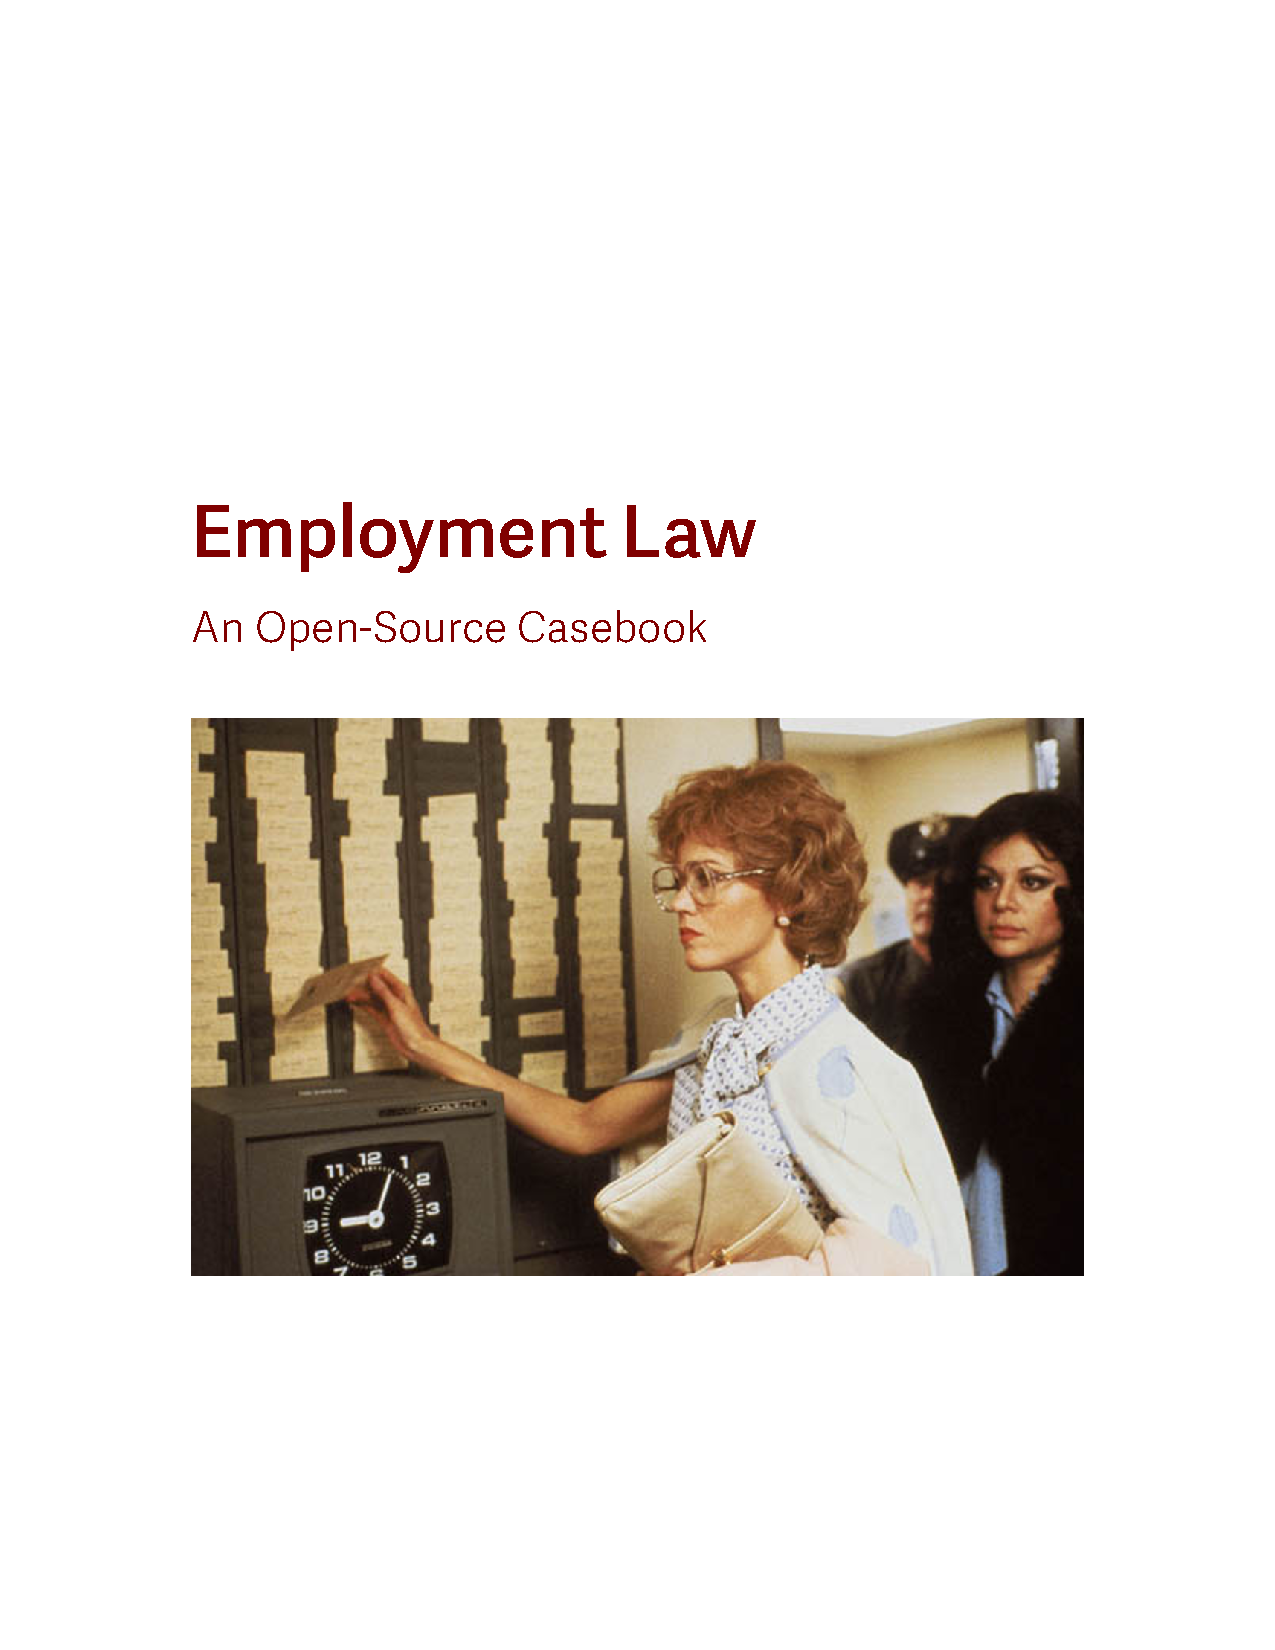
\includepdf{bookcover.pdf}\clearpage}{}

\blankpage

\frontmatter

% Frontispiece
\thispagestyle{empty}

\begin{figure}
\centering
\includegraphics[width=1\textwidth]{../img/frontispiece.jpg}
\end{figure}

\clearpage

% Title page

\thispagestyle{empty}

\begin{flushright}

\vspace*{50mm}

{\bfseries\Huge{Employment Law}} 

{\bfseries\vspace{5mm}}

{\Large{An Open-Source Casebook}} 

\vspace{20mm}

{\normalsize{Eric M. Fink}} 

\vspace*{\fill}

\begin{small}

\rmfamily{Elon Law School}  

\rmfamily{\textit{Greensboro, North Carolina}}  

\rmfamily{\monthyear} 

\end{small}

\end{flushright}

\clearpage

% License 

\thispagestyle{empty}
\begingroup
\parindent 0pt
\vspace*{\fill}

\ccbyncsa

\begin{small}
\raggedright{This work is licensed under a Creative Commons Attribution-NonCommercial-ShareAlike 4.0 International License.} \\
\url{https://creativecommons.org/licenses/by-nc-sa/4.0/}

\vspace{1em}

Eric M. Fink\\
Associate Professor of Law \\
Elon University School of Law \\
Greensboro, North Carolina 27408 \\
\url{https://www.emfink.net/ElonLaw/}

\vspace{1em}

Source code: \url{https://github.com/EricMFink/EmploymentLaw}

\itshape{version 4.1, \monthyear}

\end{small}
\endgroup

\clearpage

% Epigraph 

\thispagestyle{empty}

\topskip0pt
\vspace*{\fill}
\openepigraph{Workin' 9 to 5, what a way to make a livin'. Barely
gettin' by, it's all takin' and no givin'. They just use your mind and
they never give you credit. It's enough to drive you crazy if you let
it.}{Dolly Parton}{9 to 5}
\vspace*{\fill}

% Preface 
\chapter*{Preface}

This book presents judicial opinions, statutes and regulations, and other material pertaining to the law governing employment and labor relations. Topics covered include establishing an employment relationship; recruitment and hiring; supervisory control and employee autonomy; union representation and concerted activity; confidentiality and competition; wages and hours; employee health and workplace injuries; and termination of employment.

Most of the materials reproduced here are in the public domain; excerpts from copyrighted materials are included for teaching purposes under the fair use doctrine. Materials have been redacted to omit passages not pertinent to the learning objectives. Judicial opinions have also been "cleaned up" for ease of reading.\footnote{\textit{See} Jack Metzler, {\textit{Cleaning Up Quotations}}, 18 J. App. Prac. \& Process 143 (2017) (proposing "cleaned up" parenthetical for quotations from judicial opinions, to indicate the author “has removed extraneous, non-substantive material like brackets, quotation marks, ellipses, footnote reference numbers, and internal citations; may have changed capitalization without using brackets to indicate that change; and affirmatively represents that the alterations were made solely to enhance readability and that the quotation otherwise faithfully reproduces the quoted text.”)} 
\renewcommand*\contentsname{Contents}
{
\hypersetup{linkcolor=}
\setcounter{tocdepth}{1}
\tableofcontents
}

\mainmatter
\chapter{Employment as a Socio-Legal
Relationship}\label{employment-as-a-socio-legal-relationship}

\section{Feudal Roots}\label{feudal-roots}

\subsection[Regulating Labor in Medieval England
]{\texorpdfstring{Regulating Labor in Medieval England
\footnote{Source:
  \href{https://pasttense.co.uk/2016/06/18/today-in-legislative-history-ordinance-of-labourers-passed-to-stop-plebs-bettering-wagesconditions-1349/}{``Today
  in legislative history: Ordinance of Labourers passed to stop plebs
  bettering wages/conditions, 1349''}, Past Tense UK (Jun 18, 2016).}}{Regulating Labor in Medieval England }}\label{regulating-labor-in-medieval-england-laborers1349}

\begin{quote}
\emph{``Whereas late against the malice of servants, which were idle,
and not willing to serve after the pestilence, without taking excessive
wages, it was ordained by our lord the king\ldots{} that such manner of
servants \ldots{} should be bound to serve, receiving salary and wages,
accustomed in places where they ought to serve\ldots{} five or six years
before; and that the same servants refusing to serve \ldots{} should be
punished by imprisonment \ldots{}''}
\end{quote}

Between 1348 and 1351 a virulent plague known as the Black Death
devastated Europe. Historians estimate that between 30\% and 50\% of the
English population died from the disease. This dramatic loss in
population led to great changes taking place. Fields were left unsown
and unreaped. Entire villages lay abandoned. Those who had not died of
the plague were in danger of dying from starvation.

Food shortages also resulted in much higher prices. The peasants,
needing extra money to feed their families, demanded higher wages. The
landowners, desperately short of labour, often agreed to these wage
demands. The landowners were worried that if they refused, their workers
would run away and find an employer who was willing to pay these higher
wages.

The feudal system had largely restricted freedom of movement for the
poor, especially those who worked the land---the serfs. Landowners had
to keep their workforce, the source of the wealth, labouring for them by
force, or threat of force, or by law (really the same thing, since the
law was entirely in the hands of the ruling elites). They feared
rebellion (in retribution for the vicious treatment and grinding poverty
of their existence), or gradual or mass absconding to find somewhere
better---usually this meant to the towns, where conditions were laxer
and some eventually became free.

The labour shortages caused by the Black Death threatened to shatter
this tense system; the bargaining power was suddenly with the labouring
poor.

In 1348, Ralph, Earl of Stafford, and John Giffard were paying their
farm labourers one pence a day. By 1350 they were forced to increase it
to two pence a day. Other local landowners were paying three pence a
day. John Giffard warned the Earl of Stafford that there was a danger
that the serfs would leave Yalding in an effort to obtain higher wages.

Landowners like the Earl of Stafford complained to king Edward III about
having to pay these higher wages. The landowners were also worried about
the peasants roaming the country searching for better job opportunities.

The king issued the Ordinance of Labourers on June 18th 1349, in what is
seen as the beginning of English Labour law. It decreed that

\begin{itemize}
\tightlist
\item
  Everyone under 60 must work
\item
  Employers must not hire excess workers
\item
  Employers may not pay and workers may not receive wages higher than
  pre-plague levels
\item
  Food must be priced reasonably with no excess profit
\end{itemize}

The Ordinance, however, was largely ineffective---mainly because it flew
in the face of the material needs of both landowner and worker. In 1351,
Parliament attempted to reinforce the Ordinance, by passing the Statute
of Labourers Act. This law made it illegal for employers to pay wages
above the level offered in 1346.

Some employers, who were desperately short of workers tended to ignore
the law. This was especially true of those employers living in towns.
Some freemen who had skills in great demand, such as carpenters and
masons, began to leave their villages. Serfs became angry when they
heard of the wages that people were earning in towns. Some serfs legged
it, heading to towns in search of higher wages. Large numbers of serfs
went to London. Most of these serfs could only find unskilled manual
work. By 1360 over 40,000 people were living in London, swelling a poor
and often rebellious population.

Any serfs who got caught was taken back to their village and punished:
however, it was difficult and counter-productive for the lords of the
manor to punish them too harshly. Execution, imprisonment and mutilation
only made the labour shortage worse, so most runaways were fined.
Sometimes runaway serfs were branded on the forehead. The rest of the
serfs' tithing group were also fined for not stopping him or her from
running away.

The statute's changes failed to take into account the changing economic
conditions during the Black Death, and furthermore the period from which
wage levels were taken was one of economic depression in England as a
result of The Hundred Years' War. Therefore, wages during the Black
Death were set even lower to match those during this depression. In
practice, the statute was poorly enforced and unsuccessful, but it set a
precedent that distinguished between labourers who were ``able in body''
to work and those who could not work for whatever reasons. This
distinction was the genesis of ideas that resurfaced in later laws
regarding poverty and welfare.

The Ordinance and the Statute naturally enraged the peasants, who wanted
higher wages and better living standards. It is undeniable that this
ongoing attempt to put the clock back contributed to the general air of
resentment and rebellion that preceded and gave birth to the English
peasants' revolt of 1381. Similar processes happened throughout
Europe---wage caps following a labour shortage after the Black Death
resulting in popular revolts.

The Statute was poorly enforced in most areas, and farm wages in England
on average doubled between 1350 and 1450. However, it's also clear that
the breakdown of the rigid feudal system in England was to some extent
already underway, stimulated by other economic factors. That the Black
Death accelerated a move towards free labour and a more independent
class of small farmers us true; but serfdom was inefficient; it also
benefitted the King to have freer peasantry rather than serfs, as it
produced a larger tax base for national use, where serfs generally
enriched the immediate landowner.

Post-Black Death rulers in several countries promulgated laws to tackle
the problem. For instance, the French king Jean II, surnamed `the Good',
proclaimed his `Ordinance sur les métiers de la ville de Paris' on 30
January 1351. In addition to setting ceilings on prices and wages, the
ordinance included an extensive series of measures to curtail begging.
Unemployed, able-bodied men and women were required to accept any work
offered to earn their keep. Both the mendicants and the inhabitants of
Paris were prohibited from giving alms to those capable of working, and
this category excluded only the blind, the disabled, and other
`unfortunate persons'.

Despite the obvious failure of the post-Black Death labour legislation,
repressive laws regulating wages, almost always in favour of landowner,
employer and master, continued to be imposed in England; just a few --

\begin{itemize}
\tightlist
\item
  the 1563 Statute of Artificers, which controlled skilled trades by
  providing a compulsory seven years' apprenticeship, reserved the
  superior trades for the sons of the better off, empowered magistrates
  to force the unemployed to work and regulate all wages, required
  permission for a workman to transfer from one employer to another,
\item
  Another Statute of Labourers in 1603, which banned workers from being
  paid more than the rate magistrates set,
\item
  The 1800 Combination Acts, the last of a succession of laws banning
  workers from organizing together to improve wages or conditions, or
  from persuading others to strike\ldots{}
\item
  the Master and Servant Act 1823, only repealed in 1875, under which
  any worker could be leaving a job to seek another, without his boss's
  permission.
\end{itemize}

\begin{figure}[H]

{\centering \pandocbounded{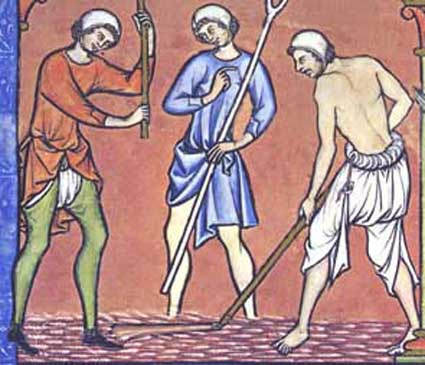
\includegraphics[keepaspectratio]{../img/medieval-labour.jpg}}

}

\caption{Medieval Laborers}

\end{figure}%

\subsection{Ordinance of Labourers,
1349}\label{ordinance-of-labourers-1349}

The king to the sheriff of Kent, greeting.

Because a great part of the people, and especially of workmen and
servants, late died of the pestilence, many seeing the necessity of
masters, and great scarcity of servants, will not serve unless they may
receive excessive wages, and some rather willing to beg in idleness,
than by labor to get their living; we, considering the grievous
incommodities, which of the lack especially of ploughmen and such
laborers may hereafter come, have upon deliberation and treaty with the
prelates and the nobles, and learned men assisting us, of their mutual
counsel ordained:

That every man and woman of our realm of England, of what condition he
be, free or bond, able in body, and within the age of threescore years,
not living in merchandise, nor exercising any craft, nor having of his
own whereof he may live, nor proper land, about whose tillage he may
himself occupy, and not serving any other, if he in convenient service,
his estate considered, be required to serve, he shall be bounden to
serve him which so shall him require; and take only the wages, livery,
meed, or salary, which were accustomed to be given in the places where
he oweth to serve, the twentieth year of our reign of England, or five
or six other commone years next before. Provided always, that the lords
be preferred before other in their bondmen or their land tenants, so in
their service to be retained; so that nevertheless the said lords shall
retain no more than be necessary for them; and if any such man or woman,
being so required to serve, will not the same do, that proved by two
true men before the sheriff or the constables of the town where the same
shall happen to be done, he shall anon be taken by them or any of them,
and committed to the next gaol, there to remain under strait keeping,
till he find surety to serve in the form aforesaid.

\emph{Item}, if any reaper, mower, or other workman or servant, of what
estate or condition that he be, retained in any man's service, do depart
from the said service without reasonable cause or license, before the
term agreed, he shall have pain of imprisonment. And that none under the
same pain presume to receive or to retain any such in his service.

\emph{Item}, that no man pay, or promise to pay, any servant any more
wages, liveries, meed, or salary than was wont, as afore is said; nor
that any in other manner shall demand or receive the same, upon pain of
doubling of that, that so shall be paid, promised, required, or
received, to him which thereof shall feel himself grieved, pursuing for
the same; and if none such will pursue, then the same to be applied to
any of the people that will pursue; and such pursuit shall be in the
court of the lord of the place where such case shall happen.

\marginnote{\begin{footnotesize}

``wapentakes'' and ``tithings'': Medieval English counties were divided
into administrative units known as ``wapentakes'' or ``hundreds''; these
were further divided into ``tithings''.

\end{footnotesize}}

\emph{Item}, if the lords of the towns or manors presume in any point to
come against this present ordinance either by them, or by their
servants, then pursuit shall be made against them in the counties,
wapentakes, tithings, or such other courts, for the treble pain paid or
promised by them or their servants in the form aforesaid; and if any
before this present ordinance hath covenanted with any so to serve for
more wages, he shall not be bound by reason of the same covenant, to pay
more than at any other time was wont to be paid to such person; nor upon
the said pain shall presume any more to pay.

\marginnote{\begin{footnotesize}

``tilers'': shipwrights.

\end{footnotesize}}

\emph{Item}, that saddlers, skinners, white-tawers, cordwainers,
tailors, smiths, carpenters, masons, tilers, carters, and all other
artificers and workmen, shall not take for their labor and workmanship
above the same that was wont to be paid to such persons the said
twentieth year, and other common years next before, as afore is said, in
the place where they shall happen to work; and if any man take more, he
shall be committed to the next gaol, in manner as afore is said.

\marginnote{\begin{footnotesize}

``hostelers'': innkeepers; ``pulters'': poultry sellers.

\end{footnotesize}}

\emph{Item}, that butchers, fishmongers, hostelers, breweres, bakers,
pulters, and all other sellers of all manner of victual, shall be bound
to sell the same victual for a reasonable price, having respect to the
price that such victual be sold at in the places adjoining, so that the
same sellers have moderate gains, and not excessive, reasonably to be
required according to the distance of the place from whence the said
victuals be carried; and if any sell such victuals in any other manner,
and thereof be convict in the manner and form aforesaid, he shall pay
the double of the same that he so received, to the party damnified, or,
in default of him, to any other that will pursue in this behalf: and the
mayors and bailiffs of cities, boroughs, merchant-towns, and others, and
of the ports and places of the sea, shall have power to inquire of all
and singular which shall in any thing offend the same, and to levy the
said pain to the use of them at whose suit such offenders shall be
convict; and in case that the same mayors or bailiffs be negligent in
doing execution of the premises, and thereof be convict before our
justices, by us to be assigned, then the same mayors and bailiffs shall
be compelled by the same justices to pay the treble of the thing so sold
to the party damnified, or to any other in default of him that will
pursue; and nevertheless toward us they shall be grievously punished.

\emph{Item}, because that many valiant beggars, as long as they may live
of begging, do refuse to labor, giving themselves to idleness and vice,
and sometime to theft and other abominations; none upon the said pain of
imprisonment shall, under the color of pity or alms, give any thing to
such, which may labor, or presume to favor them toward their desires, so
that thereby they may be compelled to labor for their necessary living.

We command you, firmly enjoining, that all and singular the premises in
the cities, boroughs, market towns, seaports, and other places in your
bailiwick, where you shall think expedient, as well within liberties as
without, you do cause to be publicly proclaimed, and to be observed and
duly put in execution aforesaid; and this by no means omit, as you
regard us and the common weal of our realm, and would save yourself
harmless. Witness the king at Westminster, the 18th day of June. By the
king himself and the whole council.

Like writs are directed to the sheriffs throughout England.

The king to the reverend father in Christ W. by the same grace bishop of
Winchester, greeting. ``Because a great part of the people,'' as before,
until ``for their necessary living,'' and then thus: And therefore we
entreat you that the premises in every of the churches, and other places
of your diocese, which you shall think expedient, you do cause to be
published; directing the parsons, vicars, ministers of such churches,
and others under you, to exhort and invite their parishioners by
salutary admonitions, to labor, and to observe the ordinances aforesaid,
as the present necessity requireth: and that you do likewise moderate
the stipendiary chaplains of your said diocese, who, as it is said, do
now in like manner refuse to serve without an excessive salary; and
compel them to serve for the accustomed salary, as it behooveth them,
under the pain of suspension and interdict. And this by no means omit,
as you regard us and the common weal of our said realm. Witness, etc. as
above. By the king himself and the whole council.

Like letters of request are directed to the several bishops of England,
and to the keeper of the spiritualities of the archbishopric of
Canterbury, during the vacancy of the see, under the same date.

\subsection{The Statute of Labourers,
1351}\label{the-statute-of-labourers-1351}

Whereas late against the malice of servants, which were idle, and not
willing to serve after the pestilence, without taking excessive wages,
it was ordained by our lord the king, and by the assent of the prelates,
nobles, and other of his council, that such manner of servants, as well
men as women, should be bound to serve, receiving salary and wages,
accustomed in places where they ought to serve in the twentieth year of
the reign of the king that now is, or five or six years before; and that
the same servants refusing to serve in such manner should be punished by
imprisonment of their bodies, as in the said statute is more plainly
contained: whereupon commissions were made to divers people in every
county to inquire and punish all them which offend against the same: and
now forasmuch as it is given the king to understand in this present
parliament, by the petition of the commonalty, that the said servants
having no regard to the said ordinance, but to their ease and singular
covetise, do withdraw themselves to serve great men and other, unless
they have livery and wages to the double or treble of that they were
wont to take the said twentieth year, and before, to the great damage of
the great men, and impoverishing of all the said commonalty, whereof the
said commonalty prayeth remedy: wherefore in the said parliament, by the
assent of the said prelates, earls, barons, and other great men, and of
the same commonalty there assembled, to refrain the malice of the said
servants, be ordained and established the things underwritten:

\marginnote{\begin{footnotesize}

``deies'': dairy maids; ``sarcling'': hoeing.

\end{footnotesize}}

\emph{First}, that carters, ploughmen, drivers of the plough, shepherds,
swineherds, deies, and all other servants, shall take liveries and
wages, accustomed the said twentieth year, or four years before; so that
in the country where wheat was wont to be given, they shall take for the
bushel ten pence, or wheat at the will of the giver, till it be
otherwise ordained. And that they be allowed to serve by a whole year,
or by other usual terms, and not by the day; and that none pay in the
time of sarcling or hay-making but a penny the day; and a mower of
meadows for the acre five pence, or by the day five pence; and reapers
of corn in the first week of August two pence, and the second three
pence, and so till the end of August, and less in the country where less
was wont to be given, without meat or drink, or other courtesy to be
demanded, given, or taken; and that such workmen bring openly in their
hands to the merchant-towns their instruments, and there shall be hired
in a common place and not privy.

\marginnote{\begin{footnotesize}

``2 d.~ob.'': The old English monetary system used units of pounds
(``l.''), shillings (``s.''), and pence (``d.''), with 1 pound = 20
shillings \& 1 shilling = 12 pence; ``ob.'' = 1/2. A ``quarter'' (8
bushels) represented a day's work for a thresher. The maximum rates of
1.5-2.5 d.~are roughly equivalent to £5-8 (\$7-11) in 2025.

\end{footnotesize}}

\emph{Item}, that none take for the threshing of a quarter of wheat or
rye over 2 d.~ob. and the quarter of barley, beans, pease, and oats, 1
d.~ob. if so much were wont to be given; and in the country where it is
used to reap by certain sheaves, and to thresh by certain bushels, they
shall take no more nor in other manner than was wont the said twentieth
year and before; and that the same servants be sworn two times in the
year before lords, stewards, bailiffs, and constables of every town, to
hold and do these ordinances; and that none of them go out of the town,
where he dwelleth in the winter, to serve the summer, if he may serve in
the same town, taking as before is said. Saving that the people of the
counties of Stafford, Lancaster and Derby, and people of Craven, and of
the marches of Wales and Scotland, and other places, may come in time of
August, and labor in other counties, and safely return, as they were
wont to do before this time: and that those, which refuse to take such
oath or to perform that that they be sworn to, or have taken upon them,
shall be put in the stocks by the said lords, stewards, bailiffs, and
constables of the towns by three days or more, or sent to the next gaol,
there to remain, till they will justify themselves. And that stocks be
made in every town for such occasion betwixt this and the feast of
Pentecost.

\marginnote{\begin{footnotesize}

``knaves'': male servants.

\end{footnotesize}}

\emph{Item}, that carpenters, masons, and tilers, and other workmen of
houses, shall not take by the day for their work, but in manner as they
were wont, that is to say: a master carpenter 3 d.~and another 2 d.; and
master free-stone mason 4 d.~and other masons 3 d.~and their servants 1
d.~ob.; tilers 3 d.~and their knaves 1 d.~ob.; and other coverers of
fern and straw 3 d.~and their knaves 1 d.~ob.; plasterers and other
workers of mudwalls, and their knaves, by the same manner, without meat
or drink, 1 s. from Easter to Saint Michael; and from that time less,
according to the rate and discretion of the justices, which should be
thereto assigned: and that they that make carriage by land or by water,
shall take no more for such carriage to be made, than they were wont the
said twentieth year, and four years before.

\marginnote{\begin{footnotesize}

``horse-smiths'': farriers; ``spurriers'': those who make spurs;
``tanners, curriers, tawers of leather'': workers involved in the
preparation of animal hides.

\end{footnotesize}}

\emph{Item}, that cordwainers and shoemakers shall not sell boots nor
shoes, nor none other thing touching their mystery, in any other manner
than they were wont the said twentieth year: item, that goldsmiths,
saddlers, horsesmiths, spurriers, tanners, curriers, tawers of leather,
tailors, and other workmen, artificers, and laborers, and all other
servants here not specified, shall be sworn before the justices, to do
and use their crafts and offices in the manner they were wont to do the
said twentieth year, and in time before, without refusing the same
because of this ordinance; and if any of the said servants, laborers,
workmen, or artificers, after such oath made, come against this
ordinance, he shall be punished by fine and ransom, and imprisonment
after the discretion of the justices.

\marginnote{\begin{footnotesize}

``harbergers'': those who provide lodging;``exigend'': a writ requiring
a defendant to appear on pain of outlawry; ``capias'': a type of arrest
warrant; ``Quintzime'': a tax known as the ``Fifteenth''.

\end{footnotesize}}

\emph{Item}, that the said stewards, bailiffs, and constables of the
said towns, be sworn before the same justices, to inquire diligently by
all the good ways they may, of all them that come against this
ordinance, and to certify the same justices of their names at all times,
when they shall come into the country to make their sessions; so that
the same justices on certificate of the same stewards, bailiffs, and
constables, of the names of the rebels, shall do them to be attached by
their body, to be before the said justices, to answer of such contempts,
so that they make fine and ransom to the king, in case they be
attainted; and moreover to be commanded to prison, there to remain till
they have found surety, to serve, and take, and do their work, and to
sell things vendible in the manner aforesaid; and in case that any of
them come against his oath, and be thereof attainted, he shall have
imprisonment of forty days; and if he be another time convict, he shall
have imprisonment of a quarter of a year, so that at every time that he
offendeth and is convict, he shall have double pain: and that the same
justices, at every time that they come {[}into the country{]}, shall
inquire of the said stewards, bailiffs, and constables, if they have
made a good and lawful certificate, or any conceal for gift,
procurement, or affinity, and punish them by fine and ransom, if they be
found guilty: and that the same justices have power to inquire and make
due punishment of the said ministers, laborers, workmen, and other
servants; and also of hostelers, harbergers, and of those that sell
victual by retail, or other things here not specified, as well at the
suit of the party, as by presentment, and to hear and determine, and put
the things in execution by the exigend after the first capias, if need
be, and to depute other under them, as many and such as they shall see
best for the keeping of the same ordinance; and that they which will sue
against such servants, workmen, laborers, {[}and artificers{]}, for
excess taken of them and they be thereof attainted at their suit, they
shall have again such excess. And in case that none will sue, to have
again such excess, then it shall be levied of the said servants,
laborers, workmen, and artificers, and delivered to the collectors of
the Quintzime, in alleviation of the towns where such excesses were
taken.

\subsection{\texorpdfstring{Karen Orren, \emph{Belated Feudalism}
(1991)}{Karen Orren, Belated Feudalism (1991)}}\label{karen-orren-belated-feudalism-1991}

When the United Stated embarked upon full-scale industrialization in the
decades following the Civil War, American labor relations were a remnant
of the ancient order, in the sense that arrangements established in
England in previous centuries were carried forward and enforced in law,
often with only slight modification, to form the framework of relations
between American employers and their employees.

\subsubsection{The order of labor}\label{the-order-of-labor}

At the most abstract level, ``feudal'' refers to the fact that the
hierarchical relation of master and servant in nineteenth-century
America was a remnant of the larger system of hierarchies that
historically had extended up and down medieval society.

Being a worker in late-nineteenth century America was still a legal
\emph{status}. By ``status,'' I refer to an established position in
society conferred upon an individual that does not arise from any
specific action or from a contract but from the individual's personal
characteristics. Nothing in American law directly stated that being a
worker was a status or that there was a legal duty to work.
Nevertheless, in every jurisdiction in the United States, not to work or
be seeking work, if one was an able-bodied person without other visible
means of support, was a crime, punishable by fine or imprisonment.
Moreover, just as being a worker was a status, this crime, known as
vagrancy, was one of the few acknowledged crimes of status in American
law---that is, one that was not defined by an action or inaction taken
in itself but was committed purely through one's personal condition, by
being a member of some predefined legal category. \ldots{}

The \href{../StatutesOfLabourers/}{Statutes of Labourers} presented the
first comprehensive scheme in which the worker's failure to work was
suppressed through the apparatus of the criminal law. In the text,
situated between the provision that victuals must be sold at reasonable
prices and the provision that a laborer accepting more wages than
customary must pay the surplus to the town, appears the following:

\begin{quote}
Item, because that many valiant {[}able-bodied{]} beggars, as long as
they may live of begging do refuse to labour, giving themselves to
idleness and vice, and sometime to theft and other abominations; none
upon the said pain of imprisonment shall, under the colour of pity of
alms, give anything to such, which may labour, or presume to favour them
towards their desires, so that therby they may be compelled to labour
for their necessary being.
\end{quote}

Those statutes, which were enforced in the British colonies, went
essentially unchanged into the eighteenth century, when they were
grafted onto the laws of the new American statutes. The same
configuration of meanings and policies in the old laws carried on into
the nineteenth century. \ldots{}

\marginnote{\begin{footnotesize}

The \emph{Institutes of the Lawes of England} are a series of legal
treatises written by Sir Edward Coke, a prominent English barrister,
judge and politician in the late sixteenth and early seventeenth
centuries.

\end{footnotesize}}

Another such principle was \emph{quicquid acquietur servo acquietur
domino} (``whatever is acquired by the servant is acquired by the
master''). That principle was continued in the law of master and
servant. A note in Hargrave's eighteeth-century edition of Coke's
\emph{Institutes} observed that the rule ``about \emph{slaves} holds
\emph{in some degree} in respect to \emph{apprentices} and
\emph{servants}'' and that it pertained with certainty to wages a worker
earned from other employment when the master had given permission to the
other employer without waiving the earnings.

By the late nineteenth century, employers in the United States could sue
workers for breach of contract for their earnings in other employment
only when it could be shown that the work had been done during hours and
activities in which the plaintiff employer had been entitled to the
worker's efforts. In an 1877 \emph{Treatise on the Law of Master and
Servant}, however, Horace Wood devoted three full pages to Hargrave's
``learned note'' and concluded that under the rule of \emph{quicquid
acquietur servo} the employer could also retain waged earned by a worker
in outside activities if the money somehow came into the employer's
hands.{\marginnote{\begin{footnotesize}Wood's treatise was an
influential work on the law governing employment in the late 19th
century. Among other things, it is widely cited as the primary source of
the employment-at-will rule. See Jay M. Feinman, The Development of the
Employment at Will Rule, 20 American Journal of Legal History 118,
125-27 (1976).\end{footnotesize}}} Moreover, even in its diluted
American form, the law expressed the employer's proprietary interest not
only in the worker's labor performed under the contract but also in all
labor that might be performed by the worker's \emph{person}, under a
different contract, The remedy went beyond simply dismissing the worker
or deducting from his wages for so many hours; it extended to the
outside earnings acquired, as if they (as an extension of the worker)
belonged to the master. Such a principle would seem incongruous not
simply with the market-model morality of enterprising employees, but
even with the more sober depictions of nineteenth-century workers as
earnest breadwinners for their families. It was eminently compatible,
however, with other features, likewise ancient, of the hierarchical
structure of employment relations during the period.

\subsubsection{The judicial governance of master and
servant}\label{the-judicial-governance-of-master-and-servant}

The links between past and present may be observed in the line of
precedents used by American judges to decide the disputes between
masters and servants and third parties that came before the courts.
\ldots{}

\marginnote{\begin{footnotesize}

Edward the Confessor was the English king from 1042 to 1066. \emph{The
Mirror of Justices} was an Anglo-Norman law text published in 1642.

\end{footnotesize}}

Regarding whether or not an employee might recover wages if asked by an
employer to work on a Sunday, Wood proceeds for several pages citing
precedents and authorities that include, among others, practice prior to
the year 500, Edward the Confessor, \emph{The Mirror of Justices}, and
Lord Coke, reaching the conclusion that the worker may not. The point is
not only that the courts followed precedent, and the precedents were
ancient, but also that there was a preestablished substance that
constituted the legal relations between the parties, which the courts
administered in the course of litigation.

As a remnant of feudalism, judicial regulation of labor relations in the
nineteenth century maintained that comprehensive sense of governance, in
which courts administered, and to a lesser extent, legislated, as well
as adjudicated. Thus, for example, by the mid-nineteenth century,
American courts, running ahead of the English, no longer permitted
employers to beat their employees. Similarly, in the 1880s, judge-made
law turned away from the assumption of an annual hiring, based on the
English model and on the prevalence of agricultural labor, to a hiring
``at-will.'' Such modifications were no doubt responsible for the
system's survival for so long, preempting interference by other agencies
of the state in unusually offensive or inconvenient circumstances. Even
so, as in the case of at-will employment, the courts continued to
prescribe labor relations, not derive them from contracts devised by the
parties. \ldots{}

Judicial governance of labor relations in the nineteenth century may
best be seen in the details of cases that came regularly to the courts
for decision and engaged central principles of the law. One principle
was the property interest that the master legally had in the worker's
labor, and indeed in all labor performed by the worker's person during
the hours for which they contracted, as mentioned earlier in regard to
the rule of \emph{quicquid acquietur servo}. That property interest was
further enforced in the action \emph{per quod servitium amisit} (``by
which the master lost the service''). In that action, the master might
claim damages from a third party for injuries to his worker that
resulted in loss of value of the worker's services, much as if the
injury had been to his chattel or machines or buildings. Blackstone,
typically, found a parallel action regarding servants in ancient Athens;
however, his discussion was more pertinent for its stress on the
traditional nonreciprocity (in the \emph{per quod} respect, as in
others) of the employment contract: The servant, having no property in
the ``company, care, or assistance of the superior,'' has no legal
redress for injuries to the master.

A second principle in nineteenth-century labor law {[}was{]} the
principle that a contract for labor was ``entire.'' Under that
principle, a worker hired for a stated job or period of time was not
legally entitled to be paid for any labor performed until the job or
term was completed. If he or she quit work without legal cause, nothing
could be recovered for the labor performed, unless the employee could
prove that the contract had been wrongfully terminated by the employer.
In that circumstance, wages could be sought by a \emph{quantum meruit}
(``for the amount owed'') suit or by a suit for damages for breach of
contract. Legal recovery was difficult, not only because of the wide
latitude given employers to discharge their workers but also because the
courts were willing to accept as a justification for dismissal virtually
any reason, even if that reason had not been stated or even known by the
employer himself at the time the dismissal took place. If the suit was
for damages, workers were required under the law to seek other
employment after their dismissal, and the court normally would deduct
any wages they received from what it required the defendant employer to
pay.

This rule made it possible for employers to goad employees into quitting
near the end of a term or pay period, and thereby benefit from their
earlier labor without having to pay. But the ``entire'' contract
principle was also basic to the full range of subject matters in dispute
between nineteenth-century employers and employees, because very often
other issues presented at law involved the question of whether or not a
worker was entitled to, or had been unjustifiably denied, payment for
his or her services. The principle was most important during the decades
prior to the Civil War, when contracts definite as to term were more
common than they would be later, but it retained its vitality after then
as well, particularly with respect to salaried workers. The principle of
hiring ``at will,'' under which either party could terminate the
contract for any reason, began to take hold in the 1880s; but in the
meantime many courts continued to apply the English rule of an assumed
annual hiring, or else held that the pay period (by the week, month,
etc.) would determine the point at which back wages could be accrued and
recovered.

\subsubsection{The province of work}\label{the-province-of-work}

The principles of hierarchy and obedience imply the existence of
jurisdictional boundaries within which authority is organized and
enforced. \ldots{}

Jurisdiction was an attribute of the master's property in the servant,
just as was the claim over the servant's labor. \ldots{} To the extent
that workplace relations under the nineteenth-century law of master and
servant were governed by the courts as a unit, the combined workplaces
constituted, concretely and not metaphorically, a single province of
work within the larger territory of American society. \ldots{}

Inside the province were the inhabitants: the employer and his
employees. Those were real persons, not their alienated labor or
functions. It was legal cause for immediate discharge to bring in an
outside worker without the master's consent to substitute for the one
hired to do the work. Once having entered the contract for services, the
worker was enlisted to be there and to perform during working hours,
upon penalty of losing back pay for an infraction. Absense by mistake of
a few days could cause discharge. The worker was not released from a
tour of duty even under such circumstances as his or her accurate
knowledge of the master's imminent bankruptcy.

Beyond the territory of the individual workplace itself, the
inhabitants, both employer and employees, engaged in what might be
referred to as interworkplace relations, that is, transactions with
other employers and employees. Although easy movement across that
boundary would seem natural in market-model societies, real crossings
encountered fixed barriers. In the case of employees, for example, a
kind of passport often was required to move from the hire of one
employer to another, which was the testimonial letter. \ldots{} In the
late nineteenth century, testimonial letters were required to obtain
employment in many major industries, and litigation arose over questions
of whether or not previous employers were under legal obligation to
furnish them, how complete and truthful they were required to be, and
how many times they had to be provided. Another barrier to employees'
free movement was that in nineteenth-century America, as in
fourteenth-century England, it was illegal to harbor servants of another
employer, that is, to employ a worker while knowing that he or she was
still under a contract of employment with someone else. It was not
essential that it be shown that the new labor had actually commenced, or
that there had been an intention to deprive the first employer of his
worker's services; the mere retention of the employee after learning
that service was due the other employer was subject to common-law suit
for damages.

Crossings of workplace boundaries met numerous other obstacles. One
obstacle was the courts' enforcement of private agreements whereby the
employee, upon departing service, agreed not to enter in business
competition with his or her former employer for a specified number or
years or over a specific territory. Another was the enforcement of what
employers claimed were implied (as well as express) contracts that
employees would not pass on to other certain ``trade secrets,'' even
though the machinery or processes were already known by others and were
unprotected by patents. Although contracts like these are certainly
familiar in the recent history of American commerce, in relations among
businessmen they had a controversial status, being regarded as illegal
restraints of trade, and were not enforced consistently until late in
the nineteenth century. But contrast, in the master-servant context,
such contracts had long been regarded as reasonable exceptions necessary
for the educative and confidential relations of employment.

Of the several protective barriers surrounding the workplace, the most
formidable in the law of master and servant was the provision against
enticement. The Statutes of Labourers provided for both civil and
criminal proceedings against any person who knowingly enticed or
persuaded a servant away from his employment by another master. By 1355,
an action of trespass on the case had developed; it provided an
independent civil remedy of damages for those same infractions within
the common law. The law of enticement is a vivid illustration of the
persistence of ancient regulations into the modern period. In the
leading antebellum case, \emph{Boston Glass Manufactory v. Binney}
(1827), plaintiffs based their argument on cases extending back as far
as 1591, and the 1591 case had been based on precedents for the action
of enticement dating from the fourteenth century.

The relations between the workplace and {[}the outside world{]} may be
seen in the developing law of employer liability for injuries caused in
the course of carrying on a trade or business. With respect to
``strangers,'' third parties outside the company, the rule of
\emph{respondeat superior} (``let the mater answer'') prevailed. That
rule meant that the employer was liable for injuries inflicted through
the fault of an employee performing his authorized duties, just as if
the injury had been caused by the employer's machine or animal. Because
prior to that time employees had themselves been held liable, unless the
particular negligent act in question had been specifically commanded or
implied by the mater, we may speculate that the newer rule \ldots{} was
an adaptation to the more attenuated forms of management typical of
larger companies.

On the other hand, \ldots{} when an injury was inflicted on an employee
through negligence of a fellow servant, the master was not responsible.
That judgment was consistent with the idea that the law must protect the
public; however, judges would not intrude in established master-servant
relations to protect the employee.

Under the rules of liability, \ldots{} employees stood in relation to
one another as an employee would to a piece of machinery. The employer
would be held liable for an injury inflicted by a fellow employee only
if the employer had not taken due care to ensure that the employee at
fault had been sufficiently skilled to perform the task, just as the
employer would be held liable if he or she had neglected to care for a
piece of machinery.

Here the worker may be seen to have had less protection than members of
the public at large against identical injuries caused by identical
accidents. By virtue of one's status as an employee of the company in
the course of whose business the injury occurred, one was unprotected
against injuries for which the company would have assumed liability had
they been inflicted on an ordinary member of the public. The evident
injustice of the fellow-servant rule, which adversely affected the
families and other associates of injured workers, as well as the workers
themselves, would eventually lead to a major revolution in torts through
the institution of workmen's compensation laws. Those laws would bring
new inroads into the domain of master and servant. However, at a time
when court decisions in other areas of the law were moving in the
direction of universal contracts, the effect of workers' compensation
laws was to enhance the status-based responsibilities of the employment
relation.

\subsubsection{The province and the
republic}\label{the-province-and-the-republic}

A final barrier against interference in the workplace was
constitutional. Labor relations were bounded by the limits of
legislative sovereignty. Regular payment of wages, and in money rather
than scrip or credit; reasons for discharge, and wages due and service
letters upon departure; removal of the fellow-servant defense against
liability for injury; shorter hours of employment---these and other
changes in the old law were obtained by workers and their political
allies in legislation, through the activities of lobbying and elections.
However, as is well known, in the majority of instances those statutes
were overturned in review by the judiciary.

Within the broad doctrine of substantive due process, ``liberty of
contract'' came closest to denying the validity of legislation per se.
Among the subjects treated by the judges under the doctrine of liberty
of contract, labor questions were in the forefront. The initial
reference to ``undue interference with men's rights of making
contracts'' appeared as a dictum in an opinion of the Illinois Supreme
Court on legislation specifying how coal should be weighed to calculate
miners' wages. The first decision to invalidate a statute as an
unconstitutional infringement on liberty of contract was
\emph{Godcharles v. Wigeman}, overturning a Pennsylvania statute
requiring iron mills to pay in cash. The first U.S. Supreme Court
decision to invalidate a state statute based on liberty of contract was
\emph{Lochner v. New York}.

The opinions in the labor decisions indicate that the judges believed
that what was at stake was no less than the moral order of things, not
merely the formal division of powers or the privileges of favorite
social groups. Their well-known opposition to ``class'' legislation was
based not so much on a sense of insult to republican principles as on
their fears that the entire system of society and politics faced
imminent demolition should the relation of master and servant be upset.
\ldots{} In \emph{Lochner}, Justice Peckham said that if an eight-hour
law for bakers were condoned, personal liberty under the constitution
would become ``visionary'':

\begin{quote}
Not only the hours of employees, but the hours of employers, could be
regulated, and doctors, lawyers, scientists, all professional men, as
well as athletes and artisans, could be forbidden to fatigue their
brains and bodies by prolonged hours of exercise, lest the fighting
strength of the state be impaired.
\end{quote}

\section{Employment as Status \&
Contract}\label{employment-as-status-contract}

\subsection{Scudder v. Woodbridge, 1 Ga. 195
(1846)}\label{scudder-v.-woodbridge-1-ga.-195-1846}

\marginnote{\begin{footnotesize}

``Plaintiff in error'': the appellant, i.e.~Scudder.

\end{footnotesize}}

Wylly Woodbridge brought an action on the case against Amos Scudder, to
recover the value of a negro boy, by the name of Ned, a carpenter,
killed on board the Ivanhoe, owned by the defendant. It was alleged in
the declaration that the property was lost by the carelessness and
mismanagement of the captain of the boat, who was employed by the owner.
This boy had been hired as a carpenter to make the trip from Savannah to
St.~Mary's, and becoming entangled in the water-wheel, in aiding to get
the boat off, he was drowned. Judge Fleming, before whom the cause was
tried in Chatham county, charged the jury, that if they found that the
death of the slave was occasioned by the negligence or want of skill in
the officers of the Ivanhoe, in the employment of Amos Scudder, that he
was liable for the loss accruing from such negligence or want of skill.
The jury returned a verdict for five hundred dollars. The defendant
below excepted to the charge of the court, and now assigns for error
that the instruction to the jury was wrong, and that the plaintiff in
error is not liable for any carelessness of his agents to those in his
employ.

The verdict of the jury having established the fact that the death of
the slave was produced by the negligence or want of skill of the
officers on board the boat, I shall not pretend to scrutinize the
testimony, but address myself at once to the inquiry, whether, conceding
the fact as found by the verdict, Scudder is liable to Woodbridge? This
question is new in our State, and well deserves the gravest
consideration.

\marginnote{\begin{footnotesize}

``The general doctrine, as contended for by counsel for plaintiff in
error'': The court is referring to the ``fellow-servant'' rule, which
precluded suits by an employee against the employer for workplace
injuries caused by co-workers. \emph{See} Farwell v. Boston \& Worcester
Railroad Co.~(Mass. 1842) in Chap. 9.

\end{footnotesize}}

The general doctrine, as contended for by counsel for plaintiff in
error, may be correct. It is distinctly laid down in \emph{Story on
Agency}, and other elementary writers, and fully sustained by the
adjudications adduced from South Carolina, Massachusetts, New York and
England. And we are disposed to recognize and adopt it, with the
cautions, limitations and restrictions in those cases. But interest to
the owner, and humanity to the slave, forbid its application to any
other than free white agents. Indeed, it cannot be extended to slaves,
\emph{ex necessitate rei}. The argument upon which the decisions
referred to mainly rest is, that public policy requires that each person
engaged on steamboats and railroads should see that every other person
employed in the same service does his duty with the utmost care and
vigilance; that every hand is qualified for his place, and that
everything connected with the line is in good order. Moreover, it is
urged, that the want of recourse on the principal will not only make
each agent more careful himself, but induce him to stimulate others to
like diligence. Can any of these considerations apply to slaves? They
dare not interfere with the business of others. They would be instantly
chastised for their impertinence. It is true that the owner, or
employer, of a slave is restrained by the Penal Code from inflicting on
him cruel, unnecessary and excessive punishment; and that all others are
forbidden to beat, whip or wound them, without sufficient cause or
provocation. But can any one doubt that if this unfortunate boy,
although shipped as a carpenter, had been ordered by the captain to
perform the perilous service in which he lost his life, and he had
refused or remonstrated, that he would have received prompt correction?
and that on the trial on a bill of indictment for a misdemeanor, his
conduct would have been deemed a sufficient justification for the
supposed offence? No! slaves dare not intermeddle with those around,
embarked in the same enterprise with themselves. Neither can they
testify against their misconduct. Neither can they exercise the salutary
discretion, left to free white agents, of quitting the employment when
matters are mismanaged, or portend evil. Whether engaged as carpenters,
bricklayers or blacksmiths---as ferrymen, wagoners, patroons or private
hands, in boats or vessels in the coasting or river navigation, on
railroads, or any other avocation---they have nothing to do but silently
serve out their appointed time, and take their lot in the mean while in
submitting to whatever risks and dangers are incident to the employment.
Bound to fidelity themselves, they do not, and cannot act as securities,
either for the care or competency of others. And what can the master
know of the condition of the vessel, road, work or machinery, where his
servant is employed, or of the skill or prudence of the persons
associated with him? No two conditions can be more different than these
two classes of agents: namely, slaves and free white citizens; and it
would be strange and extraordinary indeed if the same principle should
apply to both.

\marginnote{\begin{footnotesize}

``wholly irresponsible, \emph{civiliter}'': Enslaved persons, having the
legal status of chattel property, could neither sue nor be sued and were
thus not subject to civil liability. See, \emph{Wood v. Wood}, 2 Flip.
336 (Circuit Court, S.D. Ohio 1879).

\end{footnotesize}}

Again: a large portion of the employees at the South are either slaves
or free persons of color, wholly irresponsible, \emph{civiliter}, for
their neglect or malfeasance. The engineer on the Ivanhoe was a colored
man. Had the accident been attributable to his mismanagement, to whom
should Woodbridge have looked for redress? But we think it needless to
multiply reasons upon a point so palpable. There is one view alone which
would be conclusive with the court. The restriction of this rule is
indispensable to the welfare of the slave. In almost every occupation,
requiring combined effort, the employer necessarily intrusts it to a
variety of agents. Many of those are destitute of principle, and
bankrupt in fortune. Once let it be promulgated that the owner of
negroes hired to the numerous navigation, railroad, mining and
manufacturing companies which dot the whole country, and are rapidly
increasing---I repeat, that for any injury done to this species of
property, let it be understood and settled that the employer is not
liable, but that the owner must look for compensation to the co-servant
who occasioned the mischief, and I hesitate not to affirm, that the life
of no hired slave would be safe. As it is, the guards thrown around this
class of our population are sufficiently few and feeble. We are
altogether disinclined to lessen their number or weaken their force. We
are, therefore, cordially, confidently and unanimously agreed, and so
adjudge, that the judgment below be affirmed, with costs.

\subsection{Haskins v. Royster, 70 N.C. 600
(1874)}\label{haskins-v.-royster-70-n.c.-600-1874}

We take it to be a settled principle of law, that if one contracts upon
a consideration to render personal services for another any third person
who maliciously, that is, without a lawful justification, induces the
party who contracted to render the service to refuse to do so, is liable
to the injured party in an action for damages. It need scarcely be said
that there is nothing in this principle inconsistent with personal
freedom, else we would not find it in the laws of the freest and most
enlightened States in the world. It extends impartially to every grade
of service, from the most brilliant and best paid to the most homely,
and it shelters our nearest and tenderest domestic relations from the
interference of malicious intermeddlers. It is not derived from any idea
of property by the one party in the other, but is an inference from the
obligation of a contract freely made by competent persons.

We are relieved from any labor in finding authorities for this
principle, by a very recent decision of the Supreme Court of
Massachusetts, in which a learned and able Judge delivers the opinion of
the Court. \emph{Walker v. Cronin}, 107 Mass. 555.

That case was this: The plaintiffs declared in substance that they were
shoemakers, and employed a large number of persons as bottomers of boots
and shoes, and defendant unlawfully and intending to injure the
plaintiff in his business, persuaded and induced the persons so employed
to abandon the employment of the plaintiff, whereby plaintiff was
damaged.

A second count says that plaintiff had employed certain persons named to
make up stock into boots and shoes, and defendant well knowing, induced
said persons to refuse to make and finish such boots and shoes.

I shall make no apology for quoting copiously from this opinion, because
the high respectability of the Court, and the learning and care with
which the question is discussed, make the decision eminently an
authority.

\begin{quote}
This (the declaration) sets forth sufficiently (1) intentional and
willful acts, (2) calculated to cause damage to the plaintiffs in their
lawful business, (3) done with the unlawful purpose to cause such damage
and loss, without right or justifiable cause on the part of the
defendant (which constitutes malice), and (4) actual damage and loss
resulting.

In all cases where a man has a temporal loss or damage by the wrong of
another, he may have an action upon the case to be repaired in
damages.'' The intentional causing such loss to another, without
justifiable cause, and with the malicious purpose to inflict it, is of
itself a wrong.

Thus every one has an equal right to employ workmen in his business or
service; and if by the exercise of this right in such manner as he may
see fit, persons are induced to leave their employment elsewhere no
wrong is done to him whose employment they leave, unless a contract
exists by which such other person has a legal right to the further
continuance of their services. If such a contract exists, one who
knowingly and intentionally procures it to be violated, may be held
liable for the wrong, although he did it for the purpose of promoting
his own business.

Every one has a right to enjoy the fruits and advantages of his own
enterprise, industry, skill, and credit. He has no right to be protected
against competition; but he has a right to be free from malicious and
wanton interference, disturbance or annoyance. If disturbance or loss
come as a result of competition, or the exercise of like rights by
others, it is \emph{damnum absque injuria}, unless some superior right
by contract or otherwise is interfered with. But if it come from the
merely wanton or malicious acts of others, without the justification of
competition of the service of any interest or lawful purpose, it then
stands upon a different footing, and falls within the principle of the
authorities first referred to.

It is a familiar and well established doctrine of the law upon the
relation of master and servant, that one who entices away a servant, or
induces him to leave his master, may be held liable in damages therefor,
provided there exists a valid contract for continued service known to
the defendant. It has sometimes been supposed that the doctrine sprang
from the English statute of laborers, and was confined to menial
service. But we are satisfied that it is founded upon the legal right
derived from the contract, and not merely upon the relation of master
and servant, and that it applies to all contracts of employment, if not
to contracts of every description.
\end{quote}

It is suggested, (for we did not have the benefit of an argument for the
defendant,) that in the present case the contract between the plaintiff
and Eastwood and Wilkerson is unreasonable and therefore void. We cannot
suppose it to be contended that this Court, or any Court, when there is
no suggestion of fraud, can inquire whether the reward agreed to be paid
to a workman is the highest that he might have got in the market, and to
declare the contract void, or to make a new one if it thought not to be
the highest. No Court can make itself the guardian of persons \emph{sui
juris}. That would be an assumption inconsistent with their freedom. We
suppose the objection to a point to that part of the contract which is,
in substance, that if either party of the second part, or any person for
whom they contract, shall misbehave \emph{in the opinion of the party of
the first part}, such misbehaving party shall quit the premises
\emph{and forfeit to the party of the first part} all his interest in
the common crop.

It is said that these provisions make the plaintiff a judge in his own
cause, which the law will not allow, and that they are manifestly so
oppressive and fraudulent as to avoid the whole contract. This
proposition will be found on examination to go much too far even as
between the parties to the contract, and to have no application as
between one of the parties and a malicious intermeddler, as the
defendant must, in this stage of the case, be considered.

It is not necessary to decide what would be the effect of such a
stipulation in an action on the contract between the parties to it. But
as there seems to be some misconception of the law of such a case, and
as although there are numerous authorities on the question, it is not
yet of ``familiar learning'' in our Courts, a few observations will more
conveniently lead us to the question actually presented.

The authorities are conclusive that the parties to a contract, if there
be no fraud or concealment of the interest, may agree to make a person
interested, or even one of the parties an arbitrator to decide all
controversies which may arise under the contract, and such agreement
will be valid and effectual.

These authorities unquestionably establish that such stipulations are
not void or voidable, even as between the parties, and it has never been
supposed or contended that they made the whole contract void; as even if
void themselves, they are clearly separable from the other parts. Either
party, therefore, could maintain an action on this contract.

It is important however to notice, that none of these authorities goes
to the length of holding, that if after the contractors had duly
performed all or a part of the work, the plaintiff had \emph{mala fide},
or without lawful cause, discharged them, they could not recover upon
the contract. The power attempted to be reserved cannot have any greater
effect than to make the discharge \emph{prima facie} lawful, if so much
as that.

Contracts with such stipulations as we find in the present, are not to
be commended as precedents. Such stipulations are unusual; they answer
no useful purpose, and suggest an intent (perhaps in this case untruly)
to take some improper advantage, and to exact from the employees a
degree of personal deference and respect, beyond that civil and
courteous deportment which every man owes to his fellow in every
relation in life. To this extent, a mutual duty is implied in every
contract which creates the relation of master and servant. If the
servant fails in due respect, the master may discharge him, and so, if
the master fails, the servant will be justified in quitting the
employment.

Again it is suggested, that the contractors of the second part in this
contract are \emph{croppers}, and not servants. By cropper, I understand
a laborer who is to be paid for his labor by being given a proportion of
the crop. But such a person is not a tenant, for he has no estate in the
land, nor in the crop until the landlord assigns him his share. He is as
much a servant as if his wages were fixed and payable in money.

It is unnecessary to discuss the question whether one who maliciously
persuaded a \emph{tenant} to abandon his holding, would not be liable in
damages for such officious intermeddling.

But whatever may be the effect of the provisions commented on, as
between the parties to the contract, the authorities are clear and
decisive that a person in the situation of the defendant, can take no
advantage from them. As the case now stands, he cannot pretend to play
the part of a chivalrous protector of defrauded ignorance. For the
present at least, he must be regarded as a malicious intermeddler, using
the word malicious in its legal sense.

There is a certain analogy among all the domestic relations, and it
would be dangerous to the repose and happiness of families if the law
permitted any man, under whatever professions of philanthropy or
charity, to sow discontent between the head of the family and its
various members, wife, children and servants. Interference with such
relations can only be justified under the most special circumstances,
and where there cannot be the slightest suspicion of a spirit of
mischief-making, or self interest.

To enable a plaintiff to recover from one who entices his servant, it is
sufficient to show \emph{a subsisting relation of service}, even if it
be determinable at will. In \emph{Keane v. Boycott}, the plaintiff sued
a recruiting officer for enticing his servant. The servant was an infant
and had been a slave in St.~Vincents where he indentured himself to
serve the plaintiff for five years. The indenture of course was void
upon a double ground, but the Court held the plaintiff entitled to
recover. ``The defendant in this case \emph{had no concern in the
relation between the plaintiff and his servant; he dissolved it
officiously}, and to speak of his conduct in the mildest terms, he
carried too far his zeal for the recruiting service.''

We are of opinion that the complaint sets forth a sufficient cause of
action.

\subsection{Pollock v. Williams, 322 U.S. 4
(1944)}\label{pollock-v.-williams-322-u.s.-4-1944}

Appellant Pollock questions the validity of a statute of the State of
Florida making it a misdemeanor to induce advances with intent to
defraud by a promise to perform labor and further making failure to
perform labor for which money has been obtained \emph{prima facie}
evidence of intent to defraud. It conflicts, he says, with the
Thirteenth Amendment to the Federal Constitution and with the
antipeonage statute enacted by Congress thereunder. Claims also are made
under the due process and equal protection clauses of the Fourteenth
Amendment which we find it unnecessary to consider.

Pollock was arrested January 5, 1943, on a warrant issued three days
before which charged that on the 17th of October, 1942, he did ``with
intent to injure and defraud under and by reason of a contract and
promise to perform labor and service, procure and obtain money, to-wit:
the sum of \$5.00, as advances from one J.V. O'Albora, a corporation,
contrary to the statute in such cases made and provided, and against the
peace and dignity of the State of Florida.'' He was taken before the
county judge on the same day, entered a plea of guilty, and was
sentenced to pay a fine of \$100 and in default to serve sixty days in
the county jail. He was immediately committed.

On January 11, 1943, a writ of habeas corpus was issued by the judge of
the circuit court, directed to the jail keeper, who is appellee here.
Petition for the writ challenged the constitutionality of the statutes
under which Pollock was confined and set forth that ``at the trial
aforesaid, he was not told that he was entitled to counsel, and that
counsel would be provided for him if he wished, and he did not know that
he had such right. Petitioner was without funds and unable to employ
counsel. He further avers that he did not understand the nature of the
charge against him, but understood that if he owed any money to his
prior employer and had quit his employment without paying the same, he
was guilty, which facts he admitted.'' The Sheriff's return makes no
denial of these allegations, but merely sets forth that he holds the
prisoner by virtue of the commitment ``based upon the judgment and
conviction as set forth in the petition.'' The Supreme Court of Florida
has said that ``undenied allegations of the petition are taken as
true.''

The Circuit Court held the statutes under which the case was prosecuted
to be unconstitutional and discharged the prisoner. The Supreme Court of
Florida reversed. It read our decisions in \emph{Bailey v. Alabama} and
\emph{Taylor v. Georgia} to hold that similar laws are not in conflict
with the Constitution in so far as they denounce the crime, but only in
declaring the \emph{prima facie} evidence rule. It stated that its first
impression was that the entire Florida act would fall, as did that of
Georgia, but on reflection it concluded that our decisions were called
forth by operation of the presumption, and did not condemn the
substantive part of the statute where the presumption was not brought
into play. As the prisoner had pleaded guilty, the Florida court thought
the presumption had played no part in this case, and therefore remanded
the prisoner to custody. An appeal to this Court was taken and probable
jurisdiction noted.

Florida advances no argument that the presumption section of this
statute is constitutional, nor could it plausibly do so in view of our
decisions. It contends, however, (1) that we can give no consideration
to the presumption section because it was not in fact brought into play
in the case, by reason of the plea of guilty; (2) that so severed the
section denouncing the crime is constitutional.

\subsubsection{I.}\label{i.}

These issues emerge from an historical background against which the
Florida legislation in question must be appraised.

The Thirteenth Amendment to the Federal Constitution, made in 1865,
declares that involuntary servitude shall not exist within the United
States and gives Congress power to enforce the article by appropriate
legislation. Congress on March 2, 1867, enacted that all laws or usages
of any state ``by virtue of which any attempt shall hereafter be made to
establish, maintain, or enforce, directly or indirectly, the voluntary
or involuntary service or labor of any persons as peons, in liquidation
of any debt or obligation, or otherwise,'' are null and void, and
denounced it as a crime to hold, arrest, or return a person to the
condition of peonage.

\emph{Clyatt v. United States} was a case from Florida in which the
Federal Act was used as a sword and an employer convicted under it. This
Court sustained it as constitutional and said of peonage: ``It may be
defined as a status or condition of compulsory service, based upon the
indebtedness of the peon to the master. The basal fact is indebtedness.
Peonage is sometimes classified as voluntary or involuntary, but this
implies simply a difference in the mode of origin, but none in the
character of the servitude. The one exists where the debtor voluntarily
contracts to enter the service of his creditor. The other is forced upon
the debtor by some provision of law. A clear distinction exists between
peonage and the voluntary performance of labor or rendering of services
in payment of a debt. In the latter case the debtor, though contracting
to pay his indebtedness by labor or service, and subject like any other
contractor to an action for damages for breach of that contract, can
elect at any time to break it, and no law or force compels performance
or a continuance of the service.''

Then came the twice-considered case of \emph{Bailey v. Alabama,} in
which the Act and the Constitution were raised as a shield against
conviction of a laborer under an Alabama act substantially the same as
the one before us now. Bailey, a Negro, had obtained \$15 from a
corporation on a written agreement to work for a year at \$12 per month,
\$10.75 to be paid him and \$1.25 per month to apply on his debt. In
about a month he quit. He was convicted, fined \$30, or in default
sentenced to hard labor for 20 days in lieu of the fine and 116 days on
account of costs. The Court considered that the portion of the state law
defining the crime would require proof of intent to defraud, and so did
not strike down that part; nor was it expressly sustained, nor was it
necessarily reached, for the \emph{prima facie} evidence provision had
been used to obtain a conviction. This Court held the presumption, in
such a context, to be unconstitutional.

Later came \emph{United States v. Reynolds} in which the Act of 1867 was
sword again. Reynolds and Broughton were indicted under it. The Alabama
Code authorized one under some circumstances to become surety for a
convict, pay his fine, and be reimbursed by labor. Reynolds and
Broughton each got himself a convict to work out fines and costs as a
farm hand at \$6.00 per month. After a time each convict refused to
labor further and, under the statute, each was convicted for the
refusal. This Court said, ``Thus, under pain of recurring prosecutions,
the convict may be kept at labor, to satisfy the demands of his
employer.'' It held the Alabama statute unconstitutional and employers
under it subject to prosecution.

In \emph{Taylor v. Georgia} the Federal Act was again applied as a
shield, against conviction by resort to the presumption, of a Negro
laborer, under a Georgia statute in effect like the one before us now.
We made no effort to separate valid from invalid elements in the
statute, although the substantive and procedural provisions were, as
here, in separate, and separately numbered, sections. We said, ``We
think that the sections of the Georgia Code upon which this conviction
rests are repugnant to the Thirteenth Amendment and to the Act of 1867,
and that the conviction must therefore be reversed.'' Only recently in a
case from Northern Florida a creditor-employer was indicted under the
Federal Act for arresting a debtor to peonage, and we sustained the
indictment. \emph{United States v. Gaskin.}

These cases decided by this Court under the Act of 1867 came either from
Florida or one of the adjoining states. And these were but a part of the
stir caused by the Federal Antipeonage Act and its enforcement in this
same region. This is not to intimate that this section, more than
others, was sympathetic with peonage, for this evil has never had
general approval anywhere, and its sporadic appearances have been
neither sectional nor racial. It is mentioned, however, to indicate that
the Legislature of Florida acted with almost certain knowledge in
designing its successive ``labor fraud'' acts in relation to our series
of peonage decisions. The present Act is the latest of a lineage, in
which its antecedents were obviously associated with the practice of
peonage. This history throws some light on whether the present state act
is one ``by virtue of which any attempt shall hereafter be made'' to
``enforce involuntary servitude,'' in which event the Federal Act
declares it void.

In 1891, the Legislature created an offense of two elements: obtaining
money or property upon a false promise to perform service, and
abandonment of service without just cause and without restitution of
what had been obtained. In 1905, this Court decided \emph{Clyatt v.
United States,} indicating that any person, including public officers,
even if acting under state law, might be guilty of violating the Federal
Act. In 1907, the Florida Legislature enacted a new statute, nearly
identical in terms with that of Alabama. In 1911, in \emph{Bailey v.
Alabama,} this Court held such an act unconstitutional. In 1913, the
Florida Legislature repealed the 1907 act, but re-enacted in substance
the section denouncing the crime, omitting the presumption of intent
from the failure to perform the service or make restitution. In 1919,
the Florida Supreme Court held this act, standing alone, void under the
authority of \emph{Bailey v. Alabama.} Whereupon, at the session of
1919, the present statute was enacted, including the \emph{prima facie}
evidence provisions, notwithstanding these decisions by the Supreme
Court of Florida and by this Court. The Supreme Court of Florida later
upheld a conviction under this statute on a plea of guilty, but declined
to pass on the presumption section, because, as in the present case, the
plea of guilty was thought to make its consideration unnecessary. The
statute was re-enacted without substantial change in 1941. Again in 1943
it was re-enacted despite the fact that the year before we held a very
similar Georgia statute unconstitutional in its entirety.

\subsubsection{II.}\label{ii.}

The State contends that we must exclude the \emph{prima facie} evidence
provision from consideration because in fact it played no part in
producing this conviction. Such was the holding of the State Supreme
Court. We are not concluded by that holding, however, but under the
circumstances are authorized to make an independent determination.

What the prisoner actually did that constituted the crime cannot be
gleaned from the record. The charge is cast in the words of the statute
and is largely a conclusion. It affords no information except that
Pollock obtained \$5 from a corporation in connection with a promise to
work which he failed to perform, and that his doing so was fraudulent.
If the conclusion that the prisoner acted with intent to defraud rests
on facts and not on the \emph{prima facie} evidence provisions of the
statute, none are stated in the warrant or appear in the record. None
were so set forth that he could deny them. He obtained the money on the
14th of October, 1942, and the warrant was not sought until January 2,
1943. Whether the original advancement was more or less than \$5, what
he represented or promised in obtaining it, whether he worked a time and
quit, or whether he never began work at all are undisclosed. About all
that appears is that he obtained an advancement of \$5 from a
corporation and failed to keep his agreement to work it out. He admitted
those facts and the law purported to supply the element of intent. He
admitted the conclusion of guilt which the statute made \emph{prima
facie} thereon. He was fined \$20 for each dollar of his debt, and in
default of payment was required to atone for it by serving time at the
rate of less than 9¢ per day.

Especially in view of the undenied assertions in Pollock's petition we
cannot doubt that the presumption provision had a coercive effect in
producing the plea of guilty. The statute laid its undivided weight upon
him. The legislature had not even included a separability clause. Of
course the function of the \emph{prima facie} evidence section is to
make it possible to convict where proof of guilt is lacking. No one
questions that we clearly have held that such a presumption is
prohibited by the Constitution and the federal statute. The Florida
Legislature has enacted and twice re-enacted it since we so held. We
cannot assume it was doing an idle thing. Since the presumption was
known to be unconstitutional and of no use in a contested case, the only
explanation we can find for its persistent appearance in the statute is
its extra-legal coercive effect in suppressing defenses. It confronted
this defendant. There was every probability that a law so recently and
repeatedly enacted by the legislature would be followed by the trial
court, whose judge was not required to be a lawyer. The possibility of
obtaining relief by appeal was not bright, as the event proved, for
Pollock had to come all the way to this Court and was required, and
quite regularly, to post a supersedeas bond of \$500, a hundred times
the amount of his debt. He was an illiterate Negro laborer in the toils
of the law for the want of \$5. Such considerations bear importantly on
the decision of a prisoner even if aided by counsel, as Pollock was not,
whether to plead guilty and hope for leniency or to fight. It is plain
that, had his plight after conviction not aroused outside help, Pollock
himself would have been unheard in any appellate court.

In the light of its history, there is no reason to believe that the law
was generally used or especially useful merely to punish deceit. Florida
has a general and comprehensive statute making it a crime to obtain
money or property by false pretenses or commit ``gross fraud or cheat at
common law.'' These appear to authorize prosecution for even the petty
amount involved here. We can conceive reasons, even if unconstitutional
ones, which might lead well-intentioned persons to apply this Act as a
means to make otherwise shiftless men work, but if in addition to this
general fraud protection employers as a class are so susceptible to
imposition that they need extra legislation, or workmen so crafty and
subtle as to constitute a special menace, we do not know it, nor are we
advised of such facts.

We think that a state which maintains such a law in face of the court
decisions we have recited may not be heard to say that a plea of guilty
under the circumstances is not due to pressure of its statutory threat
to convict him on the presumption.

As we have seen, Florida persisted in putting upon its statute books a
provision creating a presumption of fraud from the mere nonperformance
of a contract for labor service three times after the courts ruled that
such a provision violates the prohibition against peonage. To attach no
meaning to such action, to say that legally speaking there was no such
legislation, is to be blind to fact. Since the Florida Legislature
deemed these repeated enactments to be important, we take the
Legislature at its own word. Such a provision is on the statute books
for those who are arrested for the crime, and it is on the statute books
for us in considering the practical meaning of what Florida has done.

In the view we take of the purpose and effect of this \emph{prima facie}
evidence provision it is not material whether as matter of state law it
is regarded as an independent and severable provision.

\subsubsection{III.}\label{iii.}

We are induced by the evident misunderstanding of our decisions by the
Florida Supreme Court, in what we are convinced was a conscientious and
painstaking study of them, to make more explicit the basis of
constitutional invalidity of this type of statute.

The undoubted aim of the Thirteenth Amendment as implemented by the
Antipeonage Act was not merely to end slavery but to maintain a system
of completely free and voluntary labor throughout the United States.
Forced labor in some special circumstances may be consistent with the
general basic system of free labor. For example, forced labor has been
sustained as a means of punishing crime, and there are duties such as
work on highways which society may compel. But in general the defense
against oppressive hours, pay, working conditions, or treatment is the
right to change employers. When the master can compel and the laborer
cannot escape the obligation to go on, there is no power below to
redress and no incentive above to relieve a harsh overlordship or
unwholesome conditions of work. Resulting depression of working
conditions and living standards affects not only the laborer under the
system, but every other with whom his labor comes in competition.
Whatever of social value there may be, and of course it is great, in
enforcing contracts and collection of debts, Congress has put it beyond
debate that no indebtedness warrants a suspension of the right to be
free from compulsory service. This congressional policy means that no
state can make the quitting of work any component of a crime, or make
criminal sanctions available for holding unwilling persons to labor. The
federal statutory test is a practical inquiry into the utilization of an
act as well as its mere form and terms.

Where peonage has existed in the United States it has done so chiefly by
virtue of laws like the statute in question. Whether the statute did or
did not include the presumption seems to have made little difference in
its practical effect. In 1910, in response to a resolution of the House
of Representatives, the Immigration Commission reported the results of
an investigation of peonage among immigrants in the United States. It
found that no general system of peonage existed, and that sentiment did
not support it anywhere. On the other hand, it found sporadic cases of
probable peonage in every state in the Union except Oklahoma and
Connecticut. It pointed out that ``there has probably existed in Maine
the most complete system of peonage in the entire country,'' in the
lumber camps. In 1907, Maine enacted a statute, applicable only to
lumber operations but in its terms very like the section of the Florida
statute we are asked to separate and save. The law was enforcible in
local courts not of record. The Commission pointed out that the Maine
statute, unlike that of Minnesota and the statutes of other states in
the West and South, did not contain a \emph{prima facie} evidence
provision. But as a practical matter the statute led to the same result.

The fraud which such statutes purport to penalize is not the concealment
or misrepresentation of existing facts, such as financial condition,
ownership of assets, or data relevant to credit. They either penalize
promissory representations which relate to future action and conduct or
they penalize a misrepresentation of the present intent or state of mind
of the laborer. In these ``a hair perhaps divides the false and true.''
Of course there might be provable fraud even in such matters. One might
engage for the same period to several employers, collecting an advance
from each, or he might work the same trick of hiring out and collecting
in advance again and again, or otherwise provide proof that fraud was
his design and purpose. But in not one of the cases to come before this
Court under the antipeonage statute has there been evidence of such
subtlety or design. In each there was the same story, a necessitous and
illiterate laborer, an agreement to work for a small wage, a trifling
advance, a breach of contract to work. In not one has there been proof
from which we fairly could say whether the Negro never intended to work
out the advance, or quit because of some real or fancied grievance, or
just got tired. If such statutes have ever on even one occasion been put
to a worthier use in the records of any state court, it has not been
called to our attention. If this is the visible record, it is hardly to
be assumed that the off-the-record uses are more benign.

It is a mistake to believe that in dealing with statutes of this type we
have held the presumption section to be the only source of invalidity.
On the contrary, the substantive section has contributed largely to the
conclusion of unconstitutionality of the presumption section. The latter
in a different context might not be invalid. Indeed, we have sustained
the power of the state to enact an almost identical presumption of
fraud, but in transactions that did not involve involuntary labor to
discharge a debt. \emph{James-Dickinson Farm Mortgage Co.~v. Harry.}
Absent this feature any objection to \emph{prima facie} evidence or
presumption statutes of the state can arise only under the Fourteenth
Amendment, rather than under the Thirteenth. In deciding peonage cases
under the latter this Court has been as careful to point out the broad
power of the state to create presumptions as it has to point out its
power to punish frauds. It ``has frequently recognized the general power
of every legislature to prescribe the evidence which shall be received,
and the effect of that evidence in the courts of its own government. In
the exercise of this power numerous statutes have been enacted providing
that proof of one fact shall be \emph{prima facie} evidence of the main
fact in issue; and where the inference is not purely arbitrary and there
is a rational relation between the two facts, and the accused is not
deprived of a proper opportunity to submit all the facts bearing upon
the issue, it has been held that such statutes do not violate the
requirements of due process of law.'' \emph{Bailey v. Alabama.} But the
Court added that ``the State may not in this way interfere with matters
withdrawn from its authority by the Federal Constitution or subject an
accused to conviction for conduct which it is powerless to proscribe.''
And it proceeded to hold that the presumption, when coupled with the
other section, transgressed those limits, for while it appeared to
punish fraud the inevitable effect of the law was to punish failure to
perform labor contracts.

In \emph{Taylor v. Georgia} both sections of the Act were held
unconstitutional. There the State relied on the presumption to convict.
But it was not denied that a state has power reasonably to prescribe the
\emph{prima facie} inferences to be drawn from circumstantial evidence.
It was the substance of the crime to establish which the presumption was
invoked that gave a forbidden aspect to that method of short-cutting the
road to conviction. The decision striking down both sections was not, as
the Supreme Court of Florida thought, a casual and unconsidered use of
the plural. Mr.~Justice Byrnes knew whereof he spoke;
unconstitutionality inhered in the substantive quite as much as in the
procedural section and no part of the invalid statute could be separated
to be salvaged. Where in the same substantive context the State
threatens by statute to convict on a presumption, its inherent coercive
power is such that we are constrained to hold that it is equally useful
in attempts to enforce involuntary service in discharge of a debt, and
the whole is invalid.

It is true that in each opinion dealing with statutes of this type this
Court has expressly recognized the right of the state to punish fraud,
even in matters of this kind, by statutes which do not either in form or
in operation lend themselves to sheltering the practice of peonage.
Deceit is not put beyond the power of the state because the cheat is a
laborer nor because the device for swindling is an agreement to labor.
But when the state undertakes to deal with this specialized form of
fraud, it must respect the constitutional and statutory command that it
may not make failure to labor in discharge of a debt any part of a
crime. It may not directly or indirectly command involuntary servitude,
even if it was voluntarily contracted for.

From what we have said about the practical considerations which are
relevant to the inquiry whether any particular state act conflicts with
the Antipeonage Act of 1867 because it is one by which ``any attempt
shall hereafter be made to establish, maintain or enforce'' the
prohibited servitude, it is apparent that we should not pass on
hypothetical acts. Reservation of the question of the validity of an act
unassociated with a presumption now, as heretofore, does not denote
approval. The Supreme Court of Florida has held such an act standing
alone unconstitutional. A considerable recorded experience would merit
examination in relation to any specific labor fraud act. We do not enter
upon the inquiry further than the Act before us.

Another matter deserves notice. In \emph{Bailey v. Alabama} it was
observed that the law of that state did not permit the prisoner to
testify to his uncommunicated intent, which handicapped him in meeting
the presumption. In \emph{Taylor v. Georgia}, the prisoner could not be
sworn, but could and did make a statement to the jury. In this Florida
case appellee is under neither disability, but is at liberty to offer
his sworn word as against presumptions. These distinctions we think are
without consequence. As Mr.~Justice Byrnes said in \emph{Taylor v.
Georgia}, the effect of this disability ``was simply to accentuate the
harshness of an otherwise invalid statute.''

We impute to the Legislature no intention to oppress, but we are
compelled to hold that the Florida Act of 1919 as brought forward on the
statutes as §§ 817.09 and 817.10 of the Statutes of 1941 are, by virtue
of the Thirteenth Amendment and the Antipeonage Act of the United
States, null and void. The judgment of the court below is reversed and
the cause is remanded for further proceedings not inconsistent with this
opinion.

\subsection{Lochner v. New York, 198 U.S. 45
(1905)}\label{lochner-v.-new-york-198-u.s.-45-1905}

\subsubsection{Mr.~Justice Peckham, after making the foregoing statement
of the facts, delivered the opinion of the
court.}\label{mr.-justice-peckham-after-making-the-foregoing-statement-of-the-facts-delivered-the-opinion-of-the-court.}

The indictment, it will be seen, charges that the plaintiff in error
violated the one hundred and tenth section of article 8, chapter 415, of
the Laws of 1897, known as the labor law of the State of New York, in
that he wrongfully and unlawfully required and permitted an employe
working for him to work more than sixty hours in one week. There is
nothing in any of the opinions delivered in this case, either in the
Supreme Court or the Court of Appeals of the State, which construes the
section, in using the word ``required,'' as referring to any physical
force being used to obtain the labor of an employe. It is assumed that
the word means nothing more than the requirement arising from voluntary
contract for such labor in excess of the number of hours specified in
the statute. There is no pretense in any of the opinions that the
statute was intended to meet a case of involuntary labor in any form.
All the opinions assume that there is no real distinction, so far as
this question is concerned, between the words ``required'' and
``permitted.'' The mandate of the statute that ``no employe shall be
required or permitted to work,'' is the substantial equivalent of an
enactment that ``no employe shall contract or agree to work,'' more than
ten hours per day, and as there is no provision for special emergencies
the statute is mandatory in all cases. It is not an act merely fixing
the number of hours which shall constitute a legal day's work, but an
absolute prohibition upon the employer, permitting, under any
circumstances, more than ten hours work to be done in his establishment.
The employe may desire to earn the extra money, which would arise from
his working more than the prescribed time, but this statute forbids the
employer from permitting the employe to earn it.

The statute necessarily interferes with the right of contract between
the employer and employes, concerning the number of hours in which the
latter may labor in the bakery of the employer. The general right to
make a contract in relation to his business is part of the liberty of
the individual protected by the Fourteenth Amendment of the Federal
Constitution. Under that provision no State can deprive any person of
life, liberty or property without due process of law. The right to
purchase or to sell labor is part of the liberty protected by this
amendment, unless there are circumstances which exclude the right. There
are, however, certain powers, existing in the sovereignty of each State
in the Union, somewhat vaguely termed police powers, the exact
description and limitation of which have not been attempted by the
courts. Those powers, broadly stated and without, at present, any
attempt at a more specific limitation, relate to the safety, health,
morals and general welfare of the public. Both property and liberty are
held on such reasonable conditions as may be imposed by the governing
power of the State in the exercise of those powers, and with such
conditions the Fourteenth Amendment was not designed to interfere.

The State, therefore, has power to prevent the individual from making
certain kinds of contracts, and in regard to them the Federal
Constitution offers no protection. If the contract be one which the
State, in the legitimate exercise of its police power, has the right to
prohibit, it is not prevented from prohibiting it by the Fourteenth
Amendment. Contracts in violation of a statute, either of the Federal or
state government, or a contract to let one's property for immoral
purposes, or to do any other unlawful act, could obtain no protection
from the Federal Constitution, as coming under the liberty of person or
of free contract. Therefore, when the State, by its legislature, in the
assumed exercise of its police powers, has passed an act which seriously
limits the right to labor or the right of contract in regard to their
means of livelihood between persons who are \emph{sui juris} (both
employer and employe), it becomes of great importance to determine which
shall prevail---the right of the individual to labor for such time as he
may choose, or the right of the State to prevent the individual from
laboring or from entering into any contract to labor, beyond a certain
time prescribed by the State.

This court has recognized the existence and upheld the exercise of the
police powers of the States in many cases which might fairly be
considered as border ones, and it has, in the course of its
determination of questions regarding the asserted invalidity of such
statutes, on the ground of their violation of the rights secured by the
Federal Constitution, been guided by rules of a very liberal nature, the
application of which has resulted, in numerous instances, in upholding
the validity of state statutes thus assailed. Among the later cases
where the state law has been upheld by this court is that of
\emph{Holden v. Hardy}. A provision in the act of the legislature of
Utah was there under consideration, the act limiting the employment of
workmen in all underground mines or workings, to eight hours per day,
``except in cases of emergency, where life or property is in imminent
danger.'' It also limited the hours of labor in smelting and other
institutions for the reduction or refining of ores or metals to eight
hours per day, except in like cases of emergency. The act was held to be
a valid exercise of the police powers of the State. A review of many of
the cases on the subject, decided by this and other courts, is given in
the opinion. It was held that the kind of employment, mining, smelting,
etc., and the character of the employes in such kinds of labor, were
such as to make it reasonable and proper for the State to interfere to
prevent the employes from being constrained by the rules laid down by
the proprietors in regard to labor.

It will be observed that, even with regard to that class of labor, the
Utah statute provided for cases of emergency wherein the provisions of
the statute would not apply. The statute now before this court has no
emergency clause in it, and, if the statute is valid, there are no
circumstances and no emergencies under which the slightest violation of
the provisions of the act would be innocent.

It must, of course, be conceded that there is a limit to the valid
exercise of the police power by the State. There is no dispute
concerning this general proposition. Otherwise the Fourteenth Amendment
would have no efficacy and the legislatures of the States would have
unbounded power, and it would be enough to say that any piece of
legislation was enacted to conserve the morals, the health or the safety
of the people; such legislation would be valid, no matter how absolutely
without foundation the claim might be. The claim of the police power
would be a mere pretext---become another and delusive name for the
supreme sovereignty of the State to be exercised free from
constitutional restraint. This is not contended for. In every case that
comes before this court, therefore, where legislation of this character
is concerned and where the protection of the Federal Constitution is
sought, the question necessarily arises: Is this a fair, reasonable and
appropriate exercise of the police power of the State, or is it an
unreasonable, unnecessary and arbitrary interference with the right of
the individual to his personal liberty or to enter into those contracts
in relation to labor which may seem to him appropriate or necessary for
the support of himself and his family? Of course the liberty of contract
relating to labor includes both parties to it. The one has as much right
to purchase as the other to sell labor.

This is not a question of substituting the judgment of the court for
that of the legislature. If the act be within the power of the State it
is valid, although the judgment of the court might be totally opposed to
the enactment of such a law. But the question would still remain: Is it
within the police power of the State? and that question must be answered
by the court.

The question whether this act is valid as a labor law, pure and simple,
may be dismissed in a few words. There is no reasonable ground for
interfering with the liberty of person or the right of free contract, by
determining the hours of labor, in the occupation of a baker. There is
no contention that bakers as a class are not equal in intelligence and
capacity to men in other trades or manual occupations, or that they are
not able to assert their rights and care for themselves without the
protecting arm of the State, interfering with their independence of
judgment and of action. They are in no sense wards of the State. Viewed
in the light of a purely labor law, with no reference whatever to the
question of health, we think that a law like the one before us involves
neither the safety, the morals nor the welfare of the public, and that
the interest of the public is not in the slightest degree affected by
such an act. The law must be upheld, if at all, as a law pertaining to
the health of the individual engaged in the occupation of a baker. It
does not affect any other portion of the public than those who are
engaged in that occupation. Clean and wholesome bread does not depend
upon whether the baker works but ten hours per day or only sixty hours a
week. The limitation of the hours of labor does not come within the
police power on that ground.

It is a question of which of two powers or rights shall prevail---the
power of the State to legislate or the right of the individual to
liberty of person and freedom of contract. The mere assertion that the
subject relates though but in a remote degree to the public health does
not necessarily render the enactment valid. The act must have a more
direct relation, as a means to an end, and the end itself must be
appropriate and legitimate, before an act can be held to be valid which
interferes with the general right of an individual to be free in his
person and in his power to contract in relation to his own labor.

We think the limit of the police power has been reached and passed in
this case. There is, in our judgment, no reasonable foundation for
holding this to be necessary or appropriate as a health law to safeguard
the public health or the health of the individuals who are following the
trade of a baker. If this statute be valid, and if, therefore, a proper
case is made out in which to deny the right of an individual, \emph{sui
juris,} as employer or employe, to make contracts for the labor of the
latter under the protection of the provisions of the Federal
Constitution, there would seem to be no length to which legislation of
this nature might not go.

We think that there can be no fair doubt that the trade of a baker, in
and of itself, is not an unhealthy one to that degree which would
authorize the legislature to interfere with the right to labor, and with
the right of free contract on the part of the individual, either as
employer or employe. In looking through statistics regarding all trades
and occupations, it may be true that the trade of a baker does not
appear to be as healthy as some other trades, and is also vastly more
healthy than still others. To the common understanding the trade of a
baker has never been regarded as an unhealthy one. Very likely
physicians would not recommend the exercise of that or of any other
trade as a remedy for ill health. Some occupations are more healthy than
others, but we think there are none which might not come under the power
of the legislature to supervise and control the hours of working
therein, if the mere fact that the occupation is not absolutely and
perfectly healthy is to confer that right upon the legislative
department of the Government. It might be safely affirmed that almost
all occupations more or less affect the health. There must be more than
the mere fact of the possible existence of some small amount of
unhealthiness to warrant legislative interference with liberty. It is
unfortunately true that labor, even in any department, may possibly
carry with it the seeds of unhealthiness. But are we all, on that
account, at the mercy of legislative majorities? A printer, a tinsmith,
a locksmith, a carpenter, a cabinetmaker, a dry goods clerk, a bank's, a
lawyer's or a physician's clerk, or a clerk in almost any kind of
business, would all come under the power of the legislature, on this
assumption. No trade, no occupation, no mode of earning one's living,
could escape this all-pervading power, and the acts of the legislature
in limiting the hours of labor in all employments would be valid,
although such limitation might seriously cripple the ability of the
laborer to support himself and his family. In our large cities there are
many buildings into which the sun penetrates for but a short time in
each day, and these buildings are occupied by people carrying on the
business of bankers, brokers, lawyers, real estate, and many other kinds
of business, aided by many clerks, messengers, and other employes. Upon
the assumption of the validity of this act under review, it is not
possible to say that an act, prohibiting lawyers' or bank clerks, or
others, from contracting to labor for their employers more than eight
hours a day, would be invalid. It might be said that it is unhealthy to
work more than that number of hours in an apartment lighted by
artificial light during the working hours of the day; that the
occupation of the bank clerk, the lawyer's clerk, the real estate clerk,
or the broker's clerk in such offices is therefore unhealthy, and the
legislature in its paternal wisdom must, therefore, have the right to
legislate on the subject of and to limit the hours for such labor, and
if it exercises that power and its validity be questioned, it is
sufficient to say, it has reference to the public health; it has
reference to the health of the employes condemned to labor day after day
in buildings where the sun never shines; it is a health law, and
therefore it is valid, and cannot be questioned by the courts.

It is also urged, pursuing the same line of argument, that it is to the
interest of the State that its population should be strong and robust,
and therefore any legislation which may be said to tend to make people
healthy must be valid as health laws, enacted under the police power. If
this be a valid argument and a justification for this kind of
legislation, it follows that the protection of the Federal Constitution
from undue interference with liberty of person and freedom of contract
is visionary, wherever the law is sought to be justified as a valid
exercise of the police power. Scarcely any law but might find shelter
under such assumptions, and conduct, properly so called, as well as
contract, would come under the restrictive sway of the legislature. Not
only the hours of employes, but the hours of employers, could be
regulated, and doctors, lawyers, scientists, all professional men, as
well as athletes and artisans, could be forbidden to fatigue their
brains and bodies by prolonged hours of exercise, lest the fighting
strength of the State be impaired. We mention these extreme cases
because the contention is extreme. We do not believe in the soundness of
the views which uphold this law. On the contrary, we think that such a
law as this, although passed in the assumed exercise of the police
power, and as relating to the public health, or the health of the
employes named, is not within that power, and is invalid. The act is
not, within any fair meaning of the term, a health law, but is an
illegal interference with the rights of individuals, both employers and
employes, to make contracts regarding labor upon such terms as they may
think best, or which they may agree upon with the other parties to such
contracts. Statutes of the nature of that under review, limiting the
hours in which grown and intelligent men may labor to earn their living,
are mere meddlesome interferences with the rights of the individual, and
they are not saved from condemnation by the claim that they are passed
in the exercise of the police power and upon the subject of the health
of the individual whose rights are interfered with, unless there be some
fair ground, reasonable in and of itself, to say that there is material
danger to the public health or to the health of the employes, if the
hours of labor are not curtailed. If this be not clearly the case the
individuals, whose rights are thus made the subject of legislative
interference, are under the protection of the Federal Constitution
regarding their liberty of contract as well as of person; and the
legislature of the State has no power to limit their right as proposed
in this statute. All that it could properly do has been done by it with
regard to the conduct of bakeries, as provided for in the other sections
of the act, above set forth. These several sections provide for the
inspection of the premises where the bakery is carried on, with regard
to furnishing proper wash-rooms and water-closets, apart from the
bakeroom, also with regard to providing proper drainage, plumbing and
painting; the sections, in addition, provide for the height of the
ceiling, the cementing or tiling of floors, where necessary in the
opinion of the factory inspector, and for other things of that nature;
alterations are also provided for and are to be made where necessary in
the opinion of the inspector, in order to comply with the provisions of
the statute. These various sections may be wise and valid regulations,
and they certainly go to the full extent of providing for the
cleanliness and the healthiness, so far as possible, of the quarters in
which bakeries are to be conducted. Adding to all these requirements, a
prohibition to enter into any contract of labor in a bakery for more
than a certain number of hours a week, is, in our judgment, so wholly
beside the matter of a proper, reasonable and fair provision, as to run
counter to that liberty of person and of free contract provided for in
the Federal Constitution.

It was further urged on the argument that restricting the hours of labor
in the case of bakers was valid because it tended to cleanliness on the
part of the workers, as a man was more apt to be cleanly when not
overworked, and if cleanly then his ``output'' was also more likely to
be so. What has already been said applies with equal force to this
contention. We do not admit the reasoning to be sufficient to justify
the claimed right of such interference. The State in that case would
assume the position of a supervisor, or \emph{pater familias,} over
every act of the individual, and its right of governmental interference
with his hours of labor, his hours of exercise, the character thereof,
and the extent to which it shall be carried would be recognized and
upheld. In our judgment it is not possible in fact to discover the
connection between the number of hours a baker may work in the bakery
and the healthful quality of the bread made by the workman. The
connection, if any exists, is too shadowy and thin to build any argument
for the interference of the legislature. If the man works ten hours a
day it is all right, but if ten and a half or eleven his health is in
danger and his bread may be unhealthful, and, therefore, he shall not be
permitted to do it. This, we think, is unreasonable and entirely
arbitrary. When assertions such as we have adverted to become necessary
in order to give, if possible, a plausible foundation for the contention
that the law is a ``health law,'' it gives rise to at least a suspicion
that there was some other motive dominating the legislature than the
purpose to subserve the public health or welfare.

This interference on the part of the legislatures of the several States
with the ordinary trades and occupations of the people seems to be on
the increase.

It is impossible for us to shut our eyes to the fact that many of the
laws of this character, while passed under what is claimed to be the
police power for the purpose of protecting the public health or welfare,
are, in reality, passed from other motives. We are justified in saying
so when, from the character of the law and the subject upon which it
legislates, it is apparent that the public health or welfare bears but
the most remote relation to the law. The purpose of a statute must be
determined from the natural and legal effect of the language employed;
and whether it is or is not repugnant to the Constitution of the United
States must be determined from the natural effect of such statutes when
put into operation, and not from their proclaimed purpose.

It is manifest to us that the limitation of the hours of labor as
provided for in this section of the statute under which the indictment
was found, and the plaintiff in error convicted, has no such direct
relation to and no such substantial effect upon the health of the
employe, as to justify us in regarding the section as really a health
law. It seems to us that the real object and purpose were simply to
regulate the hours of labor between the master and his employes (all
being men, \emph{sui juris}), in a private business, not dangerous in
any degree to morals or in any real and substantial degree, to the
health of the employes. Under such circumstances the freedom of master
and employe to contract with each other in relation to their employment,
and in defining the same, cannot be prohibited or interfered with,
without violating the Federal Constitution.

\subsubsection{Mr.~Justice Holmes,
dissenting.}\label{mr.-justice-holmes-dissenting.}

This case is decided upon an economic theory which a large part of the
country does not entertain. If it were a question whether I agreed with
that theory, I should desire to study it further and long before making
up my mind. But I do not conceive that to be my duty, because I strongly
believe that my agreement or disagreement has nothing to do with the
right of a majority to embody their opinions in law. It is settled by
various decisions of this court that state constitutions and state laws
may regulate life in many ways which we as legislators might think as
injudicious or if you like as tyrannical as this, and which equally with
this interfere with the liberty to contract. Sunday laws and usury laws
are ancient examples. A more modern one is the prohibition of lotteries.
The liberty of the citizen to do as he likes so long as he does not
interfere with the liberty of others to do the same, which has been a
shibboleth for some well-known writers, is interfered with by school
laws, by the Post Office, by every state or municipal institution which
takes his money for purposes thought desirable, whether he likes it or
not. The Fourteenth Amendment does not enact Mr.~Herbert Spencer's
Social Statics. The other day we sustained the Massachusetts vaccination
law. United States and state statutes and decisions cutting down the
liberty to contract by way of combination are familiar to this court.
Two years ago we upheld the prohibition of sales of stock on margins or
for future delivery in the constitution of California. The decision
sustaining an eight hour law for miners is still recent. Some of these
laws embody convictions or prejudices which judges are likely to share.
Some may not. But a constitution is not intended to embody a particular
economic theory, whether of paternalism and the organic relation of the
citizen to the State or of \emph{laissez faire.} It is made for people
of fundamentally differing views, and the accident of our finding
certain opinions natural and familiar or novel and even shocking ought
not to conclude our judgment upon the question whether statutes
embodying them conflict with the Constitution of the United States.

General propositions do not decide concrete cases. The decision will
depend on a judgment or intuition more subtle than any articulate major
premise. But I think that the proposition just stated, if it is
accepted, will carry us far toward the end. Every opinion tends to
become a law. I think that the word liberty in the Fourteenth Amendment
is perverted when it is held to prevent the natural outcome of a
dominant opinion, unless it can be said that a rational and fair man
necessarily would admit that the statute proposed would infringe
fundamental principles as they have been understood by the traditions of
our people and our law. It does not need research to show that no such
sweeping condemnation can be passed upon the statute before us. A
reasonable man might think it a proper measure on the score of health.
Men whom I certainly could not pronounce unreasonable would uphold it as
a first installment of a general regulation of the hours of work.
Whether in the latter aspect it would be open to the charge of
inequality I think it unnecessary to discuss.

\subsection{West Coast Hotel Co.~v. Parrish, 300 U.S. 379
(1937)}\label{west-coast-hotel-co.-v.-parrish-300-u.s.-379-1937}

This case presents the question of the constitutional validity of the
minimum wage law of the State of Washington.

The Act, entitled ``Minimum Wages for Women,'' authorizes the fixing of
minimum wages for women and minors. It provides:

\begin{quote}
SECTION 1. The welfare of the State of Washington demands that women and
minors be protected from conditions of labor which have a pernicious
effect on their health and morals. The State of Washington, therefore,
exercising herein its police and sovereign power declares that
inadequate wages and unsanitary conditions of labor exert such
pernicious effect.
\end{quote}

\begin{quote}
SEC. 2. It shall be unlawful to employ women or minors in any industry
or occupation within the State of Washington under conditions of labor
detrimental to their health or morals; and it shall be unlawful to
employ women workers in any industry within the State of Washington at
wages which are not adequate for their maintenance.
\end{quote}

\begin{quote}
SEC. 3. There is hereby created a commission to be known as the
`Industrial Welfare Commission' for the State of Washington, to
establish such standards of wages and conditions of labor for women and
minors employed within the State of Washington, as shall be held
hereunder to be reasonable and not detrimental to health and morals, and
which shall be sufficient for the decent maintenance of women.
\end{quote}

Further provisions required the Commission to ascertain the wages and
conditions of labor of women and minors within the State. Public
hearings were to be held. If after investigation the Commission found
that in any occupation, trade or industry the wages paid to women were
``inadequate to supply them necessary cost of living and to maintain the
workers in health,'' the Commission was empowered to call a conference
of representatives of employers and employees together with
disinterested persons representing the public. The conference was to
recommend to the Commission, on its request, an estimate of a minimum
wage adequate for the purpose above stated, and on the approval of such
a recommendation it became the duty of the Commission to issue an
obligatory order fixing minimum wages. Any such order might be reopened
and the question reconsidered with the aid of the former conference or a
new one. Special licenses were authorized for the employment of women
who were ``physically defective or crippled by age or otherwise,'' and
also for apprentices, at less than the prescribed minimum wage.

The appellant conducts a hotel. The appellee Elsie Parrish was employed
as a chambermaid and (with her husband) brought this suit to recover the
difference between the wages paid her and the minimum wage fixed
pursuant to the state law. The minimum wage was \$14.50 per week of 48
hours. The appellant challenged the act as repugnant to the due process
clause of the Fourteenth Amendment of the Constitution of the United
States. The Supreme Court of the State, reversing the trial court,
sustained the statute and directed judgment for the plaintiffs. The case
is here on appeal.

The appellant relies upon the decision of this Court in \emph{Adkins v.
Children's Hospital,} which held invalid the District of Columbia
Minimum Wage Act, which was attacked under the due process clause of the
Fifth Amendment. On the argument at bar, counsel for the appellees
attempted to distinguish the \emph{Adkins} case upon the ground that the
appellee was employed in a hotel and that the business of an innkeeper
was affected with a public interest. That effort at distinction is
obviously futile, as it appears that in one of the cases ruled by the
\emph{Adkins} opinion the employee was a woman employed as an elevator
operator in a hotel.

The recent case of \emph{Morehead v. New York ex rel. Tipaldo,} came
here on certiorari to the New York court, which had held the New York
minimum wage act for women to be invalid. A minority of this Court
thought that the New York statute was distinguishable in a material
feature from that involved in the \emph{Adkins} case, and that for that
and other reasons the New York statute should be sustained. But the
Court of Appeals of New York had said that it found no material
difference between the two statutes, and this Court held that the
``meaning of the statute'' as fixed by the decision of the state court
``must be accepted here as if the meaning had been specifically
expressed in the enactment.'' That view led to the affirmance by this
Court of the judgment in the \emph{Morehead} case, as the Court
considered that the only question before it was whether the
\emph{Adkins} case was distinguishable and that reconsideration of that
decision had not been sought.

We think that the question which was not deemed to be open in the
\emph{Morehead} case is open and is necessarily presented here. The
Supreme Court of Washington has upheld the minimum wage statute of that
State. It has decided that the statute is a reasonable exercise of the
police power of the State. In reaching that conclusion the state court
has invoked principles long established by this Court in the application
of the Fourteenth Amendment. The state court has refused to regard the
decision in the \emph{Adkins} case as determinative and has pointed to
our decisions both before and since that case as justifying its
position. We are of the opinion that this ruling of the state court
demands on our part a reexamination of the \emph{Adkins} case. The
importance of the question, in which many States having similar laws are
concerned, the close division by which the decision in the \emph{Adkins}
case was reached, and the economic conditions which have supervened, and
in the light of which the reasonableness of the exercise of the
protective power of the State must be considered, make it not only
appropriate, but we think imperative, that in deciding the present case
the subject should receive fresh consideration.

The principle which must control our decision is not in doubt. The
constitutional provision invoked is the due process clause of the
Fourteenth Amendment governing the States, as the due process clause
invoked in the \emph{Adkins} case governed Congress. In each case the
violation alleged by those attacking minimum wage regulation for women
is deprivation of freedom of contract. What is this freedom? The
Constitution does not speak of freedom of contract. It speaks of liberty
and prohibits the deprivation of liberty without due process of law. In
prohibiting that deprivation the Constitution does not recognize an
absolute and uncontrollable liberty. Liberty in each of its phases has
its history and connotation. But the liberty safeguarded is liberty in a
social organization which requires the protection of law against the
evils which menace the health, safety, morals and welfare of the people.
Liberty under the Constitution is thus necessarily subject to the
restraints of due process, and regulation which is reasonable in
relation to its subject and is adopted in the interests of the community
is due process.

This essential limitation of liberty in general governs freedom of
contract in particular. More than twenty-five years ago we set forth the
applicable principle in these words, after referring to the cases where
the liberty guaranteed by the Fourteenth Amendment had been broadly
described:

\begin{quote}
But it was recognized in the cases cited, as in many others, that
freedom of contract is a qualified and not an absolute right. There is
no absolute freedom to do as one wills or to contract as one chooses.
The guaranty of liberty does not withdraw from legislative supervision
that wide department of activity which consists of the making of
contracts, or deny to government the power to provide restrictive
safeguards. Liberty implies the absence of arbitrary restraint, not
immunity from reasonable regulations and prohibitions imposed in the
interests of the community.
\end{quote}

This power under the Constitution to restrict freedom of contract has
had many illustrations. That it may be exercised in the public interest
with respect to contracts between employer and employee is undeniable.
Thus statutes have been sustained limiting employment in underground
mines and smelters to eight hours a day; in requiring redemption in cash
of store orders or other evidences of indebtedness issued in the payment
of wages; in forbidding the payment of seamen's wages in advance; in
making it unlawful to contract to pay miners employed at quantity rates
upon the basis of screened coal instead of the weight of the coal as
originally produced in the mine; in prohibiting contracts limiting
liability for injuries to employees; in limiting hours of work of
employees in manufacturing establishments; and in maintaining workmen's
compensation laws. In dealing with the relation of employer and
employed, the legislature has necessarily a wide field of discretion in
order that there may be suitable protection of health and safety, and
that peace and good order may be promoted through regulations designed
to insure wholesome conditions of work and freedom from oppression.

The point that has been strongly stressed that adult employees should be
deemed competent to make their own contracts was decisively met nearly
forty years ago in \emph{Holden v.Hardy}, where we pointed out the
inequality in the footing of the parties. We said:

\begin{quote}
The legislature has also recognized the fact, which the experience of
legislators in many States has corroborated, that the proprietors of
these establishments and their operatives do not stand upon an equality,
and that their interests are, to a certain extent, conflicting. The
former naturally desire to obtain as much labor as possible from their
employes, while the latter are often induced by the fear of discharge to
conform to regulations which their judgment, fairly exercised, would
pronounce to be detrimental to their health or strength. In other words,
the proprietors lay down the rules and the laborers are practically
constrained to obey them. In such cases self-interest is often an unsafe
guide, and the legislature may properly interpose its authority.
\end{quote}

And we added that the fact ``that both parties are of full age and
competent to contract does not necessarily deprive the State of the
power to interfere where the parties do not stand upon an equality, or
where the public health demands that one party to the contract shall be
protected against himself.'' ``The State still retains an interest in
his welfare, however reckless he may be. The whole is no greater than
the sum of all the parts, and when the individual health, safety and
welfare are sacrificed or neglected, the State must suffer.''

It is manifest that this established principle is peculiarly applicable
in relation to the employment of women in whose protection the State has
a special interest. That phase of the subject received elaborate
consideration in \emph{Muller v. Oregon} (1908), where the
constitutional authority of the State to limit the working hours of
women was sustained. We emphasized the consideration that ``woman's
physical structure and the performance of maternal functions place her
at a disadvantage in the struggle for subsistence'' and that her
physical well being ``becomes an object of public interest and care in
order to preserve the strength and vigor of the race.'' We emphasized
the need of protecting women against oppression despite her possession
of contractual rights. We said that ``though limitations upon personal
and contractual rights may be removed by legislation, there is that in
her disposition and habits of life which will operate against a full
assertion of those rights. She will still be where some legislation to
protect her seems necessary to secure a real equality of right.'' Hence
she was ``properly placed in a class by herself, and legislation
designed for her protection may be sustained even when like legislation
is not necessary for men and could not be sustained.'' We concluded that
the limitations which the statute there in question ``placed upon her
contractual powers, upon her right to agree with her employer as to the
time she shall labor'' were ``not imposed solely for her benefit, but
also largely for the benefit of all.'' Again, in \emph{Quong Wing v.
Kirkendall,} in referring to a differentiation with respect to the
employment of women, we said that the Fourteenth Amendment did not
interfere with state power by creating a ``fictitious equality.'' We
referred to recognized classifications on the basis of sex with regard
to hours of work and in other matters, and we observed that the
particular points at which that difference shall be enforced by
legislation were largely in the power of the State. In later rulings
this Court sustained the regulation of hours of work of women employees
in \emph{Riley v. Massachusetts,} (factories), \emph{Miller v. Wilson,}
(hotels), and \emph{Bosley v. McLaughlin,} (hospitals).

This array of precedents and the principles they applied were thought by
the dissenting Justices in the \emph{Adkins} case to demand that the
minimum wage statute be sustained. The validity of the distinction made
by the Court between a minimum wage and a maximum of hours in limiting
liberty of contract was especially challenged. That challenge persists
and is without any satisfactory answer. As Chief Justice Taft observed:
``In absolute freedom of contract the one term is as important as the
other, for both enter equally into the consideration given and received,
a restriction as to the one is not greater in essence than the other and
is of the same kind. One is the multiplier and the other the
multiplicand.'' And Mr.~Justice Holmes, while recognizing that ``the
distinctions of the law are distinctions of degree,'' could ``perceive
no difference in the kind or degree of interference with liberty, the
only matter with which we have any concern, between the one case and the
other. The bargain is equally affected whichever half you regulate.''

The minimum wage to be paid under the Washington statute is fixed after
full consideration by representatives of employers, employees and the
public. It may be assumed that the minimum wage is fixed in
consideration of the service that are performed in the particular
occupations under normal conditions. Provision is made for special
licenses at less wages in the case of women who are incapable of full
service. The statement of Mr.~Justice Holmes in the \emph{Adkins} case
is pertinent: ``This statute does not compel anybody to pay anything. It
simply forbids employment at rates below those fixed as the minimum
requirement of health and right living. It is safe to assume that women
will not be employed at even the lowest wages allowed unless they earn
them, or unless the employer's business can sustain the burden. In short
the law in its character and operation is like hundreds of so-called
police laws that have been upheld.'' And Chief Justice Taft forcibly
pointed out the consideration which is basic in a statute of this
character: ``Legislatures which adopt a requirement of maximum hours or
minimum wages may be presumed to believe that when sweating employers
are prevented from paying unduly low wages by positive law they will
continue their business, abating that part of their profits, which were
wrung from the necessities of their employees, and will concede the
better terms required by the law; and that while in individual cases
hardship may result, the restriction will enure to the benefit of the
general class of employees in whose interest the law is passed and so to
that of the community at large.''

What can be closer to the public interest than the health of women and
their protection from unscrupulous and overreaching employers? And if
the protection of women is a legitimate end of the exercise of state
power, how can it be said that the requirement of the payment of a
minimum wage fairly fixed in order to meet the very necessities of
existence is not an admissible means to that end? The legislature of the
State was clearly entitled to consider the situation of women in
employment, the fact that they are in the class receiving the least pay,
that their bargaining power is relatively weak, and that they are the
ready victims of those who would take advantage of their necessitous
circumstances. The legislature was entitled to adopt measures to reduce
the evils of the ``sweating system,'' the exploiting of workers at wages
so low as to be insufficient to meet the bare cost of living, thus
making their very helplessness the occasion of a most injurious
competition. The legislature had the right to consider that its minimum
wage requirements would be an important aid in carrying out its policy
of protection. The adoption of similar requirements by many States
evidences a deep-seated conviction both as to the presence of the evil
and as to the means adapted to check it. Legislative response to that
conviction cannot be regarded as arbitrary or capricious, and that is
all we have to decide. Even if the wisdom of the policy be regarded as
debatable and its effects uncertain, still the legislature is entitled
to its judgment.

There is an additional and compelling consideration which recent
economic experience has brought into a strong light. The exploitation of
a class of workers who are in an unequal position with respect to
bargaining power and are thus relatively defenceless against the denial
of a living wage is not only detrimental to their health and well being
but casts a direct burden for their support upon the community. What
these workers lose in wages the taxpayers are called upon to pay. The
bare cost of living must be met. We may take judicial notice of the
unparalleled demands for relief which arose during the recent period of
depression and still continue to an alarming extent despite the degree
of economic recovery which has been achieved. It is unnecessary to cite
official statistics to establish what is of common knowledge through the
length and breadth of the land. While in the instant case no factual
brief has been presented, there is no reason to doubt that the State of
Washington has encountered the same social problem that is present
elsewhere. The community is not bound to provide what is in effect a
subsidy for unconscionable employers. The community may direct its
law-making power to correct the abuse which springs from their selfish
disregard of the public interest. The argument that the legislation in
question constitutes an arbitrary discrimination, because it does not
extend to men, is unavailing. This Court has frequently held that the
legislative authority, acting within its proper field, is not bound to
extend its regulation to all cases which it might possibly reach. The
legislature ``is free to recognize degrees of harm and it may confine
its restrictions to those classes of cases where the need is deemed to
be dearest.'' If ``the law presumably hits the evil where it is most
felt, it is not to be overthrown because there are other instances to
which it might have been applied.'' There is no ``doctrine requirement''
that the legislation should be couched in all embracing terms. This
familiar principle has repeatedly been applied to legislation which
singles out women, and particular classes of women, in the exercise of
the State's protective power. Their relative need in the presence of the
evil, no less than the existence of the evil itself, is a matter for the
legislative judgment.

Our conclusion is that the case of \emph{Adkins v. Children's Hospital}
should be, and it is, overruled.

\section{Employer Control}\label{employer-control}

\subsection{\texorpdfstring{Elizabeth Anderson, \emph{Private
Government}
(2017)}{Elizabeth Anderson, Private Government (2017)}}\label{elizabeth-anderson-private-government-2017}

Most workers in the United States are governed by dictatorships in their
work lives. Usually, those dictatorships have the legal authority to
regulate workers' off-hour lives as well---their political activities,
speech, choice of sexual partner, use of recreational drugs, alcohol,
smoking, and exercise. Because most employers exercise this off-hours
authority irregularly, arbitrarily, and without warning, most workers
are unaware of how sweeping it is. Most believe, for example, that their
boss cannot fire them for their off-hours Facebook postings, or for
supporting a political candidate their boss opposes. Yet only about half
of U.S. workers enjoy even partial protection of their off-duty speech
from employer meddling. Far fewer enjoy legal protection of their speech
on the job, except in narrowly defined circumstances. Even where they
are entitled to legal protection, as in speech promoting union activity,
their legal rights are often a virtual dead letter due to lax
enforcement: employers determined to keep out unions immediately fire
any workers who dare mention them, and the costs of litigation make it
impossible for workers to hold them accountable for this.

Employees are pervasively subject to private government, as I have
defined it. Why is this so? As far as the legal authority of the
employer to govern employees was concerned, the Industrial Revolution
did not mark a significant break. Legally speaking employers have always
been authoritarian rulers, as an extension of their patriarchal rights
to govern their households.

The Industrial Revolution moved the primary site of paid work from the
household to the factory. In principle, this could have been a
liberating moment, insofar as it opened the possibility of separating
the governance of the workplace from the governance of the home. Yet
industrial employers retained their legal entitlement to govern their
employees' domestic lives. In the early twentieth century, the Ford
Motor Company established a Sociological Department, dedicated to
inspecting employees' homes unannounced, to ensure that they were
leading orderly lives. Workers were eligible for Ford's famous \$5 daily
wage only if they kept their homes clean, ate diets deemed healthy,
abstained from drinking, used the bathtub appropriately, did not take in
boarders, avoided spending too much on foreign relatives, and were
assimilated to American cultural norms.

Workers today might breathe a sigh of relief, except that most are still
subject to employer governance of their private lives. In some cases,
this is explicit, as in employer-provided health insurance plans. Under
the Affordable Care Act (ACA), employers may impose a 30 percent premium
penalty on covered workers if they do not comply with employer-imposed
wellness programs, which may prescribe exercise programs, diets, and
abstinence from alcohol and other substances. In accordance with this
provision, Penn State University recently threatened to impose a \$100
per month surcharge on workers who did not answer a health survey that
included questions about their marital situation, sexual conduct,
pregnancy plans, and personal finances. In other cases, employer
authority over workers' off-duty lives is implicit, a by-product of the
employment-at-will rule: since employers may fire workers for any or no
reason, they may fire them for their sexual activities, partner choice,
or any other choice workers think of as private from their employer,
unless the state has enacted a law specifically forbidding employer
discrimination on these grounds. Workplace authoritarianism is still
with us.

The pro-market egalitarian aspiration toward nearly universal
self-employment aimed to liberate workers from such governance by
opening opportunities for nearly everyone to become their own boss. Why
did it fail? Why are workers subject to dictatorship? Within economics,
the theory of the firm is supposed to answer this question. It purports
to offer politically neutral, technical, economic reasons why most
production is undertaken by hierarchical organizations, with workers
subordinate to bosses, rather than by autonomous individual workers. The
theory of the firm contains important insights into the organization of
production in advanced economies. However, it fails to explain the
sweeping scope of authority that employers have over workers. What is
worse, its practitioners sometimes even deny that workers lie under the
authority of their bosses, in terms that reflect and reinforce an
illusion of workers' freedom that also characterizes much of public
discourse. Both the theory of the firm, and public discourse, are
missing an important reality: that workers are subject to their
employers' private government.

The pro-market egalitarian dream failed in part due to economies of
scale. The technological changes that drove the Industrial Revolution
involved huge concentrations of capital. A steam-powered cotton mill,
steel foundry, cement or chemical factory, or railway must be worked by
many hands. The case is no different for modern workplaces such as
airports, hospitals, pharmaceutical labs, and computer assembly
factories, as well as lower-tech workplaces such as amusement parks,
slaughterhouses, conference hotels, and big-box retail stores. The
greater efficiency of production using large, indivisible capital inputs
explains why few individual workers can afford to supply their own
capital. It explains why, contrary to the pro-market egalitarian hope,
the enterprises responsible for most production are not sole
proprietorships.

But economies of scale do not explain why production is not managed by
independent contractors acting without external supervision, who rent
their capital. One could imagine a manufacturing enterprise renting its
floor space and machinery and supplying materials to a set of
self-employed independent contractors. Each contractor would produce a
part or stage of the product for sale to contractors at the next stage
of production. The final contractor would sell the finished product to
wholesalers, or perhaps back to the capital supplier. Some New England
factories operated on a system like this from the Civil War to World War
I. They were superseded by hierarchically organized firms. According to
the theory of the firm, this is due to the excessive costs of
contracting between suppliers of factors of production. In the failed
New England system, independent contractors faced each other in a series
of bilateral monopolies, which led to opportunistic negotiations. The
demand to periodically renegotiate rates led contractors to hoard
information and delay innovation for strategic reasons. Independent
contractors wore out the machinery too quickly, failed to tightly
coordinate their production with workers at other stages of production
(leading to excess inventory of intermediate products), and lacked
incentives to innovate, both with respect to saving materials and with
respect to new products.

The modern firm solves these problems by replacing contractual relations
among workers, and between workers and owners of other factors of
production, with centralized authority. A manager, or hierarchy of
managers, issues orders to workers in pursuit of centralized objectives.
This enables close coordination of different workers and internalizes
the benefits of all types of innovation within the firm as a whole.
Managers can monitor workers to ensure that they work hard, cooperate
with fellow workers, and do not waste capital. Because they exercise
open-ended authority over workers, they can redeploy workers' efforts as
needed to implement innovations, replace absentees, and deal with
unforeseen difficulties. Authority relations eliminate the costs
associated with constant negotiation and contracting among the
participants in the firm's production. To put the point another way, the
key to the superior efficiency of hierarchy is the open-ended authority
of managers. It is impossible to specify in advance all of the
contingencies that may require an alteration in an initial understanding
of what a worker must do. Efficient employment contracts are therefore
necessarily incomplete: they do not specify precisely everything a
worker might be asked to do.

While this theory explains why firms exist and why they are constituted
by hierarchies of authority, it does not explain the sweeping scope of
employers' authority over workers in the United States. It does not
explain, for example, why employers continue to have authority over
workers' off-duty lives, given that their choice of sexual partner,
political candidate, or Facebook posting has nothing to do with
productive efficiency. Even worse, theorists of the firm appear not to
even recognize how authoritarian firm governance is. Major theorists
soft-pedal or even deny the very authority they are supposed to be
trying to explain.

Consider Ronald Coase, the originator of the theory of the firm. He
acknowledges that firms are ``islands of conscious power.'' The
employment contract is one in which the worker ``agrees to obey the
directions of an entrepreneur.'' But, he insists, ``the essence of the
contract is that it should only state the limits to the powers of the
entrepreneur.'' This suggests that the limits of the employer's powers
are an object of negotiation or at least communication between the
parties. In the vast majority of cases, outside the contexts of
collective bargaining or for higher-level employees, this is not true.
Most workers are hired without any negotiation over the content of the
employer's authority, and without a written or oral contract specifying
any limits to it. If they receive an employee handbook indicating such
limits, the inclusion of a simple disclaimer (which is standard
practice) is sufficient to nullify any implied contract exception to
at-will employment in most states. No wonder they are shocked and
outraged when their boss fires them for being too attractive, for
failing to show up at a political rally in support of the boss's favored
political candidate, even because their daughter was raped by a friend
of the boss.

What, then, determines the scope and limits of the employer's authority,
if it is not a meeting of minds of the parties? The state does so,
through a complex system of laws---not only labor law, but laws
regulating corporate governance, workplace safety, fringe benefits,
discrimination, and other matters. In the United States, the default
employment contract is employment-at-will. There are a few exceptions in
federal law to this doctrine, notably concerning discrimination, family
and medical leave, and labor union activity. For the most part, however,
at-will employment, which entitles employers to fire workers for any or
no reason, grants the employer sweeping legal authority not only over
workers' lives at work but also over their off-duty conduct. Under the
employment-at-will baseline, workers, in effect, cede all of their
rights to their employers, except those specifically guaranteed to them
by law, for the duration of the employment relationship. Employers'
authority over workers, outside of collective bargaining and a few other
contexts, such as university professors' tenure, is sweeping, arbitrary,
and unaccountable---not subject to notice, process, or appeal. The state
has established the constitution of the government of the workplace: it
is a form of private government.

Resistance to recognizing this reality appears to be widespread among
theorists of the firm. Here, for example, is what Armen Alchian and
Harold Demsetz say in their classic paper on the subject:

\begin{quote}
It is common to see the firm characterized by the power to settle issues
by fiat, by authority, or by disciplinary action. This is delusion. The
firm has no power of fiat, no authority, no disciplinary action any
different in the slightest degree from ordinary market contracting
between any two people. I can ``punish'' you only by withdrawing future
business or by seeking redress in the courts for any failure to honor
our exchange agreement. That is exactly all that any employer can do. He
can fire or sue, just as I can fire my grocer by stopping purchases from
him or sue him for delivering faulty products. What then is the content
of the presumed power to manage and assign workers to various tasks?
Exactly the same as one little consumer's power to manage and assign his
grocer to various tasks. To speak of managing, directing, or assigning
workers to various tasks is a deceptive way of noting that the employer
continually is involved in renegotiation of contracts on terms that must
be acceptable to both parties. Telling an employee to type this letter
rather than to file that document is like telling a grocer to sell me
this brand of tuna rather than that brand of bread. I have no contract
to continue to purchase from the grocer and neither the employer nor the
employee is bound by any contractual obligations to continue their
relationship.
\end{quote}

Alchian and Demsetz appear to be claiming that wherever individuals are
free to exit a relationship, authority cannot exist within it. This is
like saying that Mussolini was not a dictator, because Italians could
emigrate. While emigration rights may give governors an interest in
voluntarily restraining their power, such rights hardly dissolve it.

Alternatively, their claim might be that where the only sanctions for
disobedience are exile, or a civil suit, authority does not exist. That
would come as a surprise to those subject to the innumerable state
regulations that are backed only by civil sanctions. Nor would a state
regulation lack authority if the only sanction for violating it were to
force one out of one's job. Finally, managers have numerous other
sanctions at their disposal besides firing and suing: they can and often
do demote employees; cut their pay; assign them inconvenient hours or
too many or too few hours; assign them more dangerous, dirty, menial, or
grueling tasks; increase their pace of work; set them up to fail; and,
within very broad limits, humiliate and harass them.

Perhaps the thought is that where consent mediates the relationship
between the parties, the relationship cannot be one of subordination to
authority. That would be a surprise to the entire social contract
tradition, which is precisely about how the people can consent to
government. Or is the idea that authority exists only where subordinates
obey orders blindly and automatically? But then it exists hardly
anywhere. Even the most repressive regimes mostly rely on means besides
sheer terror and brainwashing to elicit compliance with their orders,
focusing more on persuasion and rewards.

Alchian and Demsetz may be hoodwinked by the superficial symmetry of the
employment contract: under employment-at-will, workers, too, may quit
for any or no reason. This leads them to represent quitting as
equivalent to firing one's boss. But workers have no power to remove the
boss from his position within the firm. And quitting often imposes even
greater costs on workers than being fired does, for it makes them
ineligible for unemployment insurance. It is an odd kind of
countervailing power that workers supposedly have to check their bosses'
power, when they typically suffer more from imposing it than they would
suffer from the worst sanction bosses can impose on them. Threats, to be
effective, need to be credible.

The irony is that Alchian and Demsetz are offering a theory of the firm.
The question the theory is supposed to answer is why production is not
handled entirely by market transactions among independent, self-employed
people, but rather by authority relations. That is, it is supposed to
explain why the hope of pro-market pre--Industrial Revolution
egalitarians did not pan out. Alchian and Demsetz cannot bear the full
authoritarian implications of recognizing the boundary between the
market and the firm, even in a paper devoted to explaining it. So they
attempt to extend the metaphor of the market to the internal relations
of the firm and pretend that every interaction at work is mediated by
negotiation between managers and workers. Yet the whole point of the
firm, according to the theory, is to eliminate the costs of markets---of
setting internal prices via negotiation over every transaction among
workers and between workers and managers.

Alchian and Demsetz are hardly alone. Michael Jensen and William
Meckling agree with them that authority has nothing to do with the firm;
it is merely a nexus of contracts among independent individuals. John
Tomasi, writing today, continues to promote the image of employees as
akin to independent contractors, freely negotiating the terms of their
contract with their employers, to obtain work conditions tailor-made to
their idiosyncratic specifications. While workers at the top of the
corporate hierarchy enjoy such freedom, as well as a handful of elite
athletes, entertainers, and star academics, Tomasi ignores the fact that
the vast majority of workers not represented by unions do not negotiate
terms of the employer's authority at all. Why would employers bother,
when, by state fiat, workers automatically cede all liberties not
reserved to them by the state, upon accepting an offer of work?

Not just theorists of the firm, but public discourse too, tend to
represent employees as if they were independent contractors. This makes
it seem as if the workplace is a continuation of arm's-length market
transactions, as if the labor contract were no different from a purchase
from Smith's butcher, baker, or brewer. Alchian and Demsetz are explicit
about this, in drawing the analogy of the employment relation with the
customer--grocer relation. But the butcher, baker, and brewer remain
independent from their customers after selling their goods. In the
employment contract, by contrast, the workers cannot separate themselves
from the labor they have sold; in purchasing command over labor,
employers purchase command over people.

What accounts for this error? The answer is, in part, that a
representation of what egalitarians hoped market society would deliver
for workers before the Industrial Revolution has been blindly carried
over to the post--Industrial Revolution world. People continue to deploy
the same justification of market society---that it would secure the
personal independence of workers from arbitrary authority---long after
it failed to deliver on its original aspiration. The result is a kind of
political hemiagnosia: like those patients who cannot perceive one-half
of their bodies, a large class of libertarian-leaning thinkers and
politicians, with considerable public following, cannot perceive half of
the economy: they cannot perceive the half that takes place beyond the
market, after the employment contract is accepted.

\marginnote{\begin{footnotesize}

Hemiagnosia, also known as hemispatial neglect, is a neuropsychologial
condition, resulting from brain damage after a stroke or injury, in
which a person loses awareness of objects and stimuli on one side of
their body. Oliver Sacks described one such case in his book,
\href{https://www.oliversacks.com/oliver-sacks-books/the-man-who-mistook-his-wife-for-a-hat/}{\emph{The
Man Who Mistook His Wife for a Hat}}.

\end{footnotesize}}

This tendency was reinforced by a narrowing of egalitarian vision in the
transition to the Industrial Revolution. While the Levellers and other
radicals of the mid-seventeenth century agitated against all kinds of
arbitrary government, Thomas Paine mainly narrowed his critique to state
abuses. Similarly, the Republican Party kept speaking mainly on behalf
of the interests of businesspeople and those who hoped to be in business
for themselves, even after it was clear that the overwhelming majority
of workers had no realistic prospect of attaining this status, and that
the most influential businesspeople were not, as Lincoln hoped, sole
proprietors (with at most a few employees, the majority of whom were
destined to rise to self-employed status after a few years), but
managers in large organizations, governing workers destined to be wage
laborers for their entire working lives. Thus, a political agenda that
once promised equalizing as well as liberating outcomes turned into one
that reinforced private, arbitrary, unaccountable government over the
vast majority.

Finally, nineteenth-century laissez-faire liberals, with their bizarre
combination of hostility toward state power and enthusiasm for
hyperdisciplinary total institutions, attempted to reconcile these
contradictory tendencies by limiting their focus to the entry and exit
conditions of the labor contract, while blackboxing what actually went
on in the factories. In fact, they did drive a dramatic improvement in
workers' freedom of entry and exit. Under the traditional common law of
master and servant, employees were bound to their employers by contracts
of one year (apprentices and indentured servants for longer), could quit
before then only on pain of losing all their accrued wages, and were not
entitled to keep wages from moonlighting. Other employers were forbidden
to bid for their labor while they were still under contract. Workers
were liberated from these constraints over the course of the nineteenth
century.

This liberation, as is well-known, was a double-edged sword. Employers,
too, were liberated from any obligation to employ workers. As already
noted, the worst the workers could do to the boss often involved
suffering at least as much as the worst the boss could do to them. For
the bulk of workers, who lived at the bottom of the hierarchy, this was
not much of a threat advantage, unless it was exercised collectively in
a strike. They had no realistic hope under these conditions for
liberation from workplace authoritarianism.

No wonder a central struggle of British workers in the mid-nineteenth
century was for limits on the length of the working day---even more than
for higher wages. This was true, even though workers at this period of
the Industrial Revolution were suffering through ``Engels's
pause''---the first fifty to sixty years of the Industrial Revolution
during which wages failed to grow. My focus, like theirs, is not on
issues of wages or distributive justice. It is on workers' freedom. If
the Industrial Revolution meant they could not be their own bosses at
work, at least they could try to limit the length of the working day so
that they would have some hours during which they could choose for
themselves, rather than follow someone else's orders.

That was an immediate aim of European workers' movements in the
mid-nineteenth century. As the century unfolded, workers largely
abandoned their pro-market, individualistic egalitarian dream and turned
to socialist, collectivist alternatives---that is, to restructuring the
internal governance of the workplace. The problem was that the options
open to workers consisted almost exclusively of private governments.
Laissez-faire liberals, touting the freedom of the free market, told
workers: choose your Leviathan. That is like telling the citizens of the
Communist bloc of Eastern Europe that their freedom could be secured by
a right to emigrate to any country---as long as they stayed behind the
Iron Curtain. Population movements would likely have put some pressure
on Communist rulers to soften their rule. But why should Leviathan set
the baseline against which competition took place? No liberal or
libertarian would be satisfied with a competitive equilibrium set
against this baseline, where the choice of state governments is
concerned. Workers' movements rejected it for nonstate governments as
well.

To their objection, libertarians and laissez-faire liberals had no
credible answer. Let us not fool ourselves into supposing that the
competitive equilibrium of labor relations was ever established by
politically neutral market forces mediated by pure freedom of contract,
with nothing but the free play of individuals' idiosyncratic preferences
determining the outcome. This is a delusion as great as the one that
imagines that the workplace is not authoritarian. Every competitive
equilibrium is established against a background assignment of property
rights and other rights established by the state. The state supplies the
indispensable legal infrastructure of developed economies as a kind of
public good, and is needed to do so to facilitate cooperation on the
vast scales that characterize today's rich and sophisticated economies.
Thus, it is the state that establishes the default constitution of
workplace governance. It is a form of authoritarian, private government,
in which, under employment-at-will, workers cede all their rights to
their employers, except those specifically reserved for them by law.

Freedom of entry and exit from any employment relation is not sufficient
to justify the outcome. To see this, consider an analogous case for the
law of coverture, which the state had long established as the default
marriage contract. Under coverture, a woman, upon marrying her husband,
lost all rights to own property and make contracts in her own name. Her
husband had the right to confine her movements, confiscate any wages she
might earn, beat her, and rape her. Divorce was very difficult to
obtain. The marriage contract was valid only if voluntarily accepted by
both parties. It was a contract into subjection, entailing the wife's
submission to the private government of her husband. Imagine a
modification of this patriarchal governance regime, allowing either
spouse to divorce at will and allowing any clause of the default
contract to be altered by a prenuptial agreement. This is like the
modification that laissez-faire liberals added to the private government
of the workplace. Women would certainly have sufficient reason to object
that their liberties would still not be respected under this
modification, in that it preserves a patriarchal baseline, in which men
still hold virtually all the cards. It would allow a lucky few to escape
subjection to their husbands, but that is not enough to justify the
patriarchal authority the vast majority of men would retain over their
wives. Consent to an option within a set cannot justify the option set
itself.

I do not claim that private governments at work are as powerful as
states. Their sanctioning powers are lower, and the costs of emigration
from oppressive private governments are generally lower than the costs
of emigration from states. Yet private governments impose a far more
minute, exacting, and sweeping regulation of employees than democratic
states do in any domain outside of prisons and the military. Private
governments impose controls on workers that are unconstitutional for
democratic states to impose on citizens who are not convicts or in the
military.

The negative liberties most workers enjoy de facto are considerably
greater than the ones they are legally entitled to under their
employers. Market pressures, social norms, lack of interest, and simple
decency keep most employers from exercising the full scope of their
authority. We should care nevertheless about the insecurity of
employees' liberty. They work in a state of republican unfreedom, their
liberties vulnerable to cancellation without justification, notice,
process, or appeal. That they enjoy substantially greater negative
liberty than they are legally entitled to no more justifies their lack
of republican liberty than the fact that most wives enjoyed greater
freedoms than they were legally entitled to justified coverture---or
even coverture modified by free divorce.

Suppose people find themselves under private government. This is a state
of republican unfreedom, of subjection to the arbitrary will of another.
It is also usually a state of substantial constraints on negative
liberty. By what means could people attain their freedom? One way would
be to end subjection to government altogether. When the government is a
state, this is the anarchist answer. We have seen that when the
government is an employer, the answer of many egalitarians before the
Industrial Revolution was to advance a property regime that promotes
self-employment, perhaps even to make self-employment a nearly
universally accessible opportunity, at least for men. This amounts to
promoting anarchy as the primary form of workplace order.

The theory of the firm explains why this approach cannot preserve the
productive advantages of large-scale production. Some kind of
incompletely specified authority over groups of workers is needed to
replace market relations within the firm. However, the theory of the
firm, although it explains the necessity of hierarchy, neither explains
nor justifies private government in the workplace. That the constitution
of workplace government is both arbitrary and dictatorial is not
dictated by efficiency or freedom of contract, but rather by the state.
Freedom of contract no more explains the equilibrium workplace
constitution than freedom to marry explained women's subjection to
patriarchy under coverture.

In other words, in the great contest between individualism and
collectivism regarding the mode of production, collectivism won,
decisively. Now nearly all production is undertaken by teams of workers
using large, indivisible forms of capital equipment held in common. The
activities of these teams are governed by managers according to a
centralized production plan. This was an outcome of the Industrial
Revolution, and equally much embraced by capitalists and socialists.
That advocates of capitalism continue to speak as if their preferred
system of production upholds ``individualism'' is simply a symptom of
institutional hemiagnosia, the misdeployment of a hopeful preindustrial
vision of what market society would deliver as if it described our
current reality, which replaces market relations with governance
relations across wide domains of production.

Workers in the nineteenth century turned from individualistic to
collectivist solutions to workplace governance because they saw that
interpersonal authority---governments over groups of workers---was
inescapable in the new industrial order. If government is inescapable or
necessary for solving certain important problems, the only way to make
people free under that government is to make that government a public
thing, accountable to the governed. The task is to replace private
government with public government.

When the government is a state, we have some fairly good ideas of how to
proceed: the entire history of democracy under the rule of law is a
series of experiments in how to make the government of the state a
public thing, and the people free under the state. These experiments
continue to this day.

But what if the government is an employer? Here matters are more
uncertain. There are four general strategies for advancing and
protecting the liberties and interests of the governed under any type of
government: (1) exit, (2) the rule of law, (3) substantive
constitutional rights, and (4) voice. Let us consider each in turn.

Exit is usually touted as a prime libertarian strategy for protecting
individual rights. By forcing governments to compete for subjects, exit
rights put pressure on governments to offer their subjects better deals.
``The defense against oppressive hours, pay, working conditions, or
treatment is the right to change employers.'' Given this fact, it is
surprising how comfortable some libertarians are with the validity of
contracts into slavery, from which exit is disallowed. In their view,
freedom of contract trumps the freedom of individuals under government,
or even the freedom to leave that government. While contracts into
slavery and peonage are no longer valid, other contractual barriers to
exit are common and growing. Noncompete clauses, which bar employees
from working for other employers in the same industry for a period of
years, have spread from technical professions (where nearly half of
employees are subject to them) to jobs such as sandwich maker, pesticide
sprayer, summer camp counselor, and hairstylist. While employers can no
longer hold workers in bondage, they can imprison workers' human
capital. California is one of the few states that prohibit noncompete
clauses. As the dynamism of its economy proves, such contractual
barriers to exit are not needed for economic growth, and probably
undermine it. There should be a strong legal presumption against such
barriers to exit, to protect workers' freedom to exit their employers'
government.

The rule of law is a complex ideal encompassing several protections of
subjects' liberties: (a) Authority may be exercised only through laws
duly passed and publicized in advance, rather than arbitrary orders
issued without any process. (b) Subjects are at liberty to do anything
not specifically prohibited by law. (c) Laws are generally applicable to
everyone in similar circumstances. (d) Subjects have rights of due
process before suffering any sanctions for noncompliance. Not all of
these protections, which were devised with state authority in mind, can
be readily transferred to the employment context. Most of the solutions
to problems the state must address involve regulations that leave open
to individuals a vast array of options for selecting both ends and
means. By contrast, efficient production nearly always requires close
coordination of activities according to centralized objectives, directed
by managers exercising discretionary authority. This frequently entails
that the authority of managers over workers be both intensive (limiting
workers to highly particular movements and words, not allowing them to
pursue their own personal objectives at work or even to select their own
means to a prescribed end) and incompletely specified. The state imposes
traffic laws that leave people free to choose their own destinations,
routes, and purposes. Walmart tells its drivers what they have to pick
up, when and where they have to deliver it, and what route they have to
take. In addition, managers need incompletely specified authority to
rapidly reassign different tasks to different workers to address new
circumstances. Finally, excessively costly procedural protections
against firing also discourage hiring. All these obstacles to applying
rule-of-law protections in the workplace empower employers to abuse
their authority, subject workers to humiliating treatment, and impose
excessive constraints on their freedom.

At the same time, it is easy to exaggerate the obstacles to imposing
rule-of-law protections at work. Larger organizations generally have
employee handbooks and standard practice guides that streamline
authority along legalistic lines. Equal protection and due process
rights already exist for workers in larger organizations with respect to
limited issues. A worker who has been sexually harassed by her boss
normally has recourse to intrafirm procedures for resolving her
complaint. Such protections reflect a worldwide ``blurring of
boundaries'' among business, nonprofit, and state organizations, which
appears to be driven not simply by legal changes, but by cultural
imperatives of scientific management and ideas of individual rights and
organizational responsibilities. Some but not all of these managerial
developments are salutary. They are proper subjects of investigation for
political theory, once we get beyond the subject's narrow focus on the
state.

A just workplace constitution should incorporate basic constitutional
rights, akin to a bill of rights against employers. To some extent, the
Fair Labor Standards Act, anti-discrimination laws, and other workplace
regulations already serve this function. A workers' bill of rights could
be strengthened by the addition of more robust protections of workers'
freedom to engage in off-duty activities, such as exercising their
political rights, free speech, and sexual choices. Similar protections
for employee privacy could be extended in the workplace during work
breaks. The Occupational Safety and Health Administration (OSHA)
prohibitions of particularly degrading, dangerous, and onerous working
conditions can be viewed as part of a workers' bill of rights. Nabisco
once threatened its female production line workers with three-day
suspensions for using the bathroom, and ordered them to urinate in their
clothes instead. It was only in 1998 that OSHA issued a regulation
requiring employers to recognize workers' right to use a bathroom, after
cases such as Nabisco's aroused public outrage. Workers in Europe are
protected from harassment of all kinds by anti-mobbing laws. This gives
them far more robust workplace constitutional rights than workers in the
United States, who may be legally harassed as long as their harassers do
not discriminate by race, gender, or other protected identities in
choosing their victims.

There are limits, however, to how far a bill of rights can go in
protecting workers from abuse. Because they prescribe uniformity across
workplaces, they can at best offer a minimal floor. In practice, they
are also grossly underenforced for the least advantaged workers.
Furthermore, such laws do not provide for worker participation in
governance at the firm level. They merely impose limits on employer
dictatorship.

For these reasons, there is no adequate substitute for recognizing
workers' voice in their government. Voice can more readily adapt
workplace rules to local conditions than state regulations can, while
incorporating respect for workers' freedom, interests, and dignity. Just
because workplace governance requires a hierarchy of offices does not
mean that higher officeholders must be unaccountable to the governed, or
that the governed should not play any role in managerial
decision-making. In the United States, two models for workers' voice
have received the most attention: workplace democracy and labor unions.
Workplace democracy, in the form of worker-owned and -managed firms, has
long stood as an ideal for many egalitarians. While much could be done
to devise laws more accommodating of this structure, some of its costs
may be difficult to surmount. In particular, the costs of negotiation
among workers with asymmetrical interests (for example, due to
possession of different skills) appear to be high.

In the United States, collective bargaining has been the primary way
workers have secured voice within the government of the workplace.
However, even at its peak in 1954, only 28.3 percent of workers were
represented by a labor union. Today, only 11.1 percent of all workers
and 6.6 percent of private sector workers are represented. Although laws
could be revised to make it easier for workers to organize into a union,
this does not address difficulties inherent to the U.S. labor union
model. The U.S. model organizes workers at the firm level rather than
the industry level. Firms vigorously resist unionization to avoid a
competitive disadvantage with non-unionized firms. Labor unions also
impose inefficiencies due to their monopoly power. They also take an
adversarial stance toward management---one that makes not only managers
but also many workers uncomfortable. At the same time, they often
provide the only effective voice employees have in workplace governance.

It is possible to design a workplace constitution in which workers have
a non-adversarial voice in workplace governance, without raising
concerns about monopolization. The overwhelming majority of workers in
the United States would like to have such a voice: 85 percent would like
firm governance to be ``run jointly'' by management and workers. In the
United States, such a constitution is illegal under the National Labor
Relations Act, which prohibits company unions. Yet this structure is
commonplace in Europe. Germany's system of codetermination, begun in the
Weimar era and elaborately developed since World War II, offers one
highly successful model.

It is not my intention in this lecture to defend any particular model of
worker participation in firm governance. My point is rather to expose a
deep failure in current ways of thinking about how government fits into
Americans' lives. We do not live in the market society imagined by Paine
and Lincoln, which offered an appealing vision of what a free society of
equals would look like, combining individualistic libertarian and
egalitarian ideals. Government is everywhere, not just in the form of
the state, but even more pervasively in the workplace. Yet public
discourse and much of political theory pretends that this is not so. It
pretends that the constitution of workplace government is somehow the
object of voluntary negotiation between workers and employers. This is
true only for a tiny proportion of privileged workers. The vast majority
are subject to private, authoritarian government, not through their own
choice, but through laws that have handed nearly all authority to their
employers.

\subsection{Skagerberg v. Blandin Paper Co., 266 N.W. 872 (Minn.
1936)}\label{skagerberg-v.-blandin-paper-co.-266-n.w.-872-minn.-1936}

Plaintiff is a consulting engineer, a specialist in the field of
heating, ventilating, and air conditioning. As such he had developed a
clientele bringing him a weekly income of approximately \$200.

Defendant operates a paper manufacturing plant at Grand Rapids, this
state. It had employed plaintiff in his professional capacity in 1926
and again in 1930. He was paid at the rate of \$200 per week while so
employed. Defendant was planning extensive enlargements of its plant,
the estimated expense being about \$1,000,000. Ordinarily a consulting
engineer's fees for doing the necessary planning and supervision of the
contemplated improvements would involve from \$35,000 to \$50,000.
During plaintiff's employment in 1930 there was some discussion between
the parties with respect of plaintiff's employment to take this work in
hand. At that time, too, he was negotiating with the executive officers
of Purdue University relative to taking a position as associate
professor in its department of engineering, particularly that branch
thereof relating to heating, ventilating, and air conditioning.

The Purdue position carried a salary of \$3,300 per year and required
only nine months' work in the way of instructions. This would leave
plaintiff free to continue his practice as a consulting engineer during
a period of three months of each calendar year. He was also privileged,
if he entered that position, to continue his practice as a consulting
engineer at all times insofar as his professional work at the university
permitted him so to do. In addition thereto, he was privileged to
contribute to engineering magazines and other publications. All income
from such outside engagements was to be his in addition to the stated
salary. Plaintiff considered this opportunity as one especially
attractive to him. Defendant had full knowledge of all the foregoing
facts.

On October 13, 1930, plaintiff, having received a telegram from Purdue
University offering him the position and requiring immediate acceptance
or rejection thereof, at once called an officer of defendant over the
long-distance telephone informing him of the offer and the necessity on
his part of making immediate response thereto. Defendant's officer
agreed that if plaintiff would reject the Purdue offer and also agree to
purchase the home of defendant's power superintendent it would give
plaintiff permanent employment at a salary of \$600 per month. Relying
thereon, plaintiff rejected the Purdue offer and immediately thereafter
moved to Grand Rapids and there entered upon the performance of his
duties under this arrangement. He later entered into a contract for the
purchase of the superintendent's home. Appropriate to note is the fact
that these negotiations were entirely oral and over the long-distance
telephone, plaintiff being at Minneapolis and defendant's officer at
Grand Rapids. The only writing between the parties is a letter written
on October 14, 1930, reading thus:

\begin{quote}
Blandin Paper Co.~``Grand Rapids, Minn.''Attention: Mr.~C.K. Andrews
``Gentlemen:
\end{quote}

\begin{quote}
In accordance with our conversation yesterday when our agreement was
settled regarding my position with your company, I have wired Purdue
rejecting their offer. Under the circumstances it was impossible for us
to get together on a written agreement; I had to wire Purdue at once.
However, I am making this move on the assumption that there will be no
difficulty in working out our agreement when I get up to Grand Rapids.
\end{quote}

\begin{quote}
Propositions like the one Purdue made are very rare and I am turning it
down since I feel that the opportunities with you for applying my past
experience are very attractive, the essential consideration being,
however, that the job will be a permanent one.
\end{quote}

\begin{quote}
According to the understanding we have, I am to take over Mr.~Kull's
duties as Power Superintendent and serve also as Mechanical Engineer for
your plant, supervising the mechanical construction and maintenance work
and other mechanical technical matters. Mr.~Kull is to remain for long
enough period, about six months, to permit me to get my work organized
and get acquainted with the details of his work. If the proposed new
construction work is started within that time it may develop that
Mr.~Kull may remain until that is completed after which he will leave
and I take over his duties. As an accommodation to him when he leaves
town I am to purchase his house.
\end{quote}

\begin{quote}
My salary is to be six hundred dollars (\$600.00) per month and you are
to pay my moving expenses to Grand Rapids.
\end{quote}

\begin{quote}
Very truly yours, ``RS/m R. Skagerberg.
\end{quote}

Plaintiff rendered the services for which he was thus engaged
``dutifully, faithfully and to the complete satisfaction of the
defendant and was paid the agreed salary, except as to a voluntary
reduction, up to September 1, 1932,'' when, so the complaint alleges, he
was ``wrongfully, unlawfully and wilfully'' discharged from further
employment, although ``ready, willing and able to perform.'' By reason
of the alleged breach of contract he claims to have suffered general
damages in the amount of \$25,000, and for this he prays judgment.

From what has been stated it is clear that the issue raised by the
demurrer is simply this: Do the allegations set forth in the complaint
show anything more than employment of plaintiff by defendant subject to
termination at the will of either party?

The words ``permanent employment'' have a well established meaning in
the law:

\begin{quote}
In case the parties to a contract of service expressly agree that the
employment shall be `permanent' the law implies, not that the engagement
shall be continuous or for any definite period, but that the term being
indefinite the hiring is merely at will.
\end{quote}

The difficult question presented is whether the allegations set forth in
the complaint bring this case within an exception to the rule stated. We
find in 18 R.C.L. p.~510, the following statement:

\begin{quote}
Under some circumstances, however, `permanent' employment will be held
to contemplate a continuous engagement to endure as long as the employer
shall be engaged in business and have work for the employe to do and the
latter shall perform the service satisfactorily. This seems to be the
established rule in case the employe purchases the employment with a
valuable consideration outside the services which he renders from day to
day.
\end{quote}

And in 35 A.L.R. 1434, it is said:

\begin{quote}
It has been held that where an employe has given a good consideration in
addition to his services, an agreement to hire him permanently should,
in the absence of other terms or circumstances to the contrary, continue
so long as the employe is able and willing to do his work
satisfactorily.
\end{quote}

Plaintiff cites and relies upon \emph{Carnig v. Carr}, 167 Mass. 544;
\emph{Roxana Petroleum Co.~v. Rice}, 109 Okla. 161; \emph{Pierce v.
Tennessee C. I. R. Co.} 173 U.S. 1, and other cases of similar import. A
brief discussion of the cited cases upon which plaintiff relies may be
helpful.

In \emph{Carnig v. Carr}, plaintiff had been engaged in business for
himself as an enameler. Defendant was a business competitor. Being such,
and for his own advantage, defendant persuaded plaintiff to give up his
business and sell his stock in trade to him. As consideration, in part
at least, for entering into this arrangement, defendant agreed to employ
plaintiff permanently at a stated salary, his work for defendant being
the same as that in which plaintiff had been engaged. It is clear that
what defendant sought and accomplished was to get rid of his competitor
in business upon a promise on his part to give plaintiff permanent
employment. The resulting situation amounted to the same thing in
substance and effect as if plaintiff had purchased his job. Under such
circumstances there can be no doubt that the exception to the general
rule was properly invoked and applied and furnishes an illustration
thereof.

In \emph{Pierce v. Tennessee C. I. R. Co.}, plaintiff had received an
injury while employed by defendant. To settle the difficulty defendant
promised employment to plaintiff at certain stated wages and was also to
furnish certain supplies as long as his disability to do full work
continued by reason of his injury. In consideration for these promises
plaintiff released the company from all liability for damages on account
of the injuries which caused his disability. Here, too, it is clear that
plaintiff purchased from defendant his employment.

In \emph{Roxana Petroleum Co.~v. Rice}, plaintiffs Rice and Lyons were
attorneys and rendered professional services for defendant over a period
of time. They had other clients who paid them large annual retainers,
one of these being the Pierce Oil Company, from which client they
received an annual retainer of \$17,500. The attorneys were prevailed
upon by defendant to sever their connections with other clients and were
promised and paid an annual retainer of \$15,000, later increased to
\$20,000. Some time thereafter the petroleum company claimed that the
expense bills were unsatisfactory. A controversy arose, and to settle
same a compromise agreement was made. ``In this compromise agreement a
new employment contract was made. The general offices of the company had
been moved to St.~Louis. Plaintiffs were to continue their services in
representing defendant in 40 or 50 lawsuits that were then pending in
the courts of Oklahoma and Texas, and they were to continue in the
services of the company in these two states as long as the defendant
operated therein and as long as the services of the plaintiffs were
satisfactory, and pay them reasonable fees for legal as well as other
services. Later on new difficulties arose respecting the new contract.
The court in distinguishing this form of contract from the ordinary
contract of permanent employment came to the conclusion that because
plaintiffs had compromised their claims against the company, changed
their position in relation to their general practice, incurred expenses
in maintaining an office for the special services of defendant, that
thereby there was a permanent contract of employment. The court said:

\begin{quote}
We are of the opinion that from the facts and circumstances attending
the making of the contract of employment in the instant case it was the
intention of the parties that the employment was to continue as long as
the defendant was in business in Oklahoma and Texas, and the plaintiffs
were not subject to discharge without cause.
\end{quote}

With regard to that part of the new agreement which provided that
plaintiffs were to be paid as long as their services were
``satisfactory'' to defendant, the facts were such as to justify the
court in holding that defendant's claimed dissatisfaction was not
genuine but rather and only pretended. The court quoted with approval
the following statement from \emph{Electric Lighting Co.~v. Elder
Bros.}:

\begin{quote}
But the dissatisfaction must be in good faith and with the performance
of the contract. A plea of dissatisfaction with the work agreed to be
satisfactorily completed must allege the facts from which the
dissatisfaction arises. He must be in good faith dissatisfied. He cannot
avoid liability by merely alleging that he is dissatisfied. The
dissatisfaction must not be capricious nor mercenary nor result from a
design to be dissatisfied. It must exist as a fact. It must be actual,
not feigned; real, not merely a pretext to escape liability.
\end{quote}

That the court did not intend to go beyond the general rule pertaining
to such form of contract is clearly shown by the subsequent opinion
rendered in \emph{Dunn v. Birmingham S. R. Co.}, where plaintiff was
hired as defendant's exclusive agent for the sale of its products in
Tulsa, no time limit as to term of service having been provided for in
the agreement. Five months later defendant, without notice to plaintiff,
began selling its products to other retailers in Tulsa. Judgment for
plaintiff in nominal damages only was sustained on appeal.

This court has had occasion to pass upon similar questions in various
cases. Thus in \emph{Horn v. Western Land Assn.}, plaintiff had been
appointed as attorney for defendant ``at a salary of \$1,000 per year,
payable quarterly,'' and was so informed in writing. Plaintiff wrote a
letter ``accepting the appointment upon the terms offered.'' The court
determined that this constituted a contract as to which neither party,
without the other's consent, could lawfully rescind without cause during
the year.

In \emph{Bolles v. Sachs}, two written agreements were involved, neither
showing upon its face mutuality of obligation or other consideration.
The court held that the two instruments could be considered together so
as to show that one was given in consideration for the other. As thus
construed the contract amounted to one of employment providing in
substance that plaintiff was to render services for defendant as long as
he might elect to serve. The employer breached the contract and sued for
damages. The court held that the employe, never having fixed by his
election the period of service, could not recover substantial damages,
the obligation violated being too uncertain to furnish a basis for
assessment of substantial damages.

In \emph{Smith v. St.~Paul D. R. Co.}, plaintiff had been injured in the
line of his employment. In settlement of the injury he was promised
employment. In respect of the validity of such contract the court said:

\begin{quote}
The consideration for defendant's agreement to employ was paid by the
release of plaintiff's claim for damages quite as much and as
effectually as if plaintiff had actually paid cash. By releasing his
claim for damages, the plaintiff paid in advance for the privilege or
option of working for the defendant; and, having done this, he had the
right to have it remain optional with him how long he would continue to
work for the company, while it remained obligatory upon the latter to
furnish the opportunity so long as he chose to work, and was able to
properly perform the same. The plaintiff had parted with value for the
optional contract, and there was owing to him a reciprocal duty and
obligation on the part of the company.
\end{quote}

In \emph{McMullan v. Dickinson Co.}, the first syllabus paragraph of the
second opinion reads:

\begin{quote}
Plaintiff and defendant, a corporation, entered into an agreement by the
terms of which the latter employed the former as assistant manager upon
a stated yearly salary, payable in monthly instalments, said employment
to continue so long as the business of the corporation should be
continued, provided plaintiff properly and efficiently discharged his
duties, and only so long as he should own and hold in his own name 50
shares of capital stock, fully paid up, in defendant corporation.
\emph{Held}, that the period of employment was for such time as
plaintiff continued to own and hold the stock shares, not exceeding the
period during which the corporate business was being transacted, and was
fixed with sufficient definiteness; and, further, that there was no lack
of mutuality of consideration.
\end{quote}

In \emph{Newhall v. Journal Printing Co.}, action was brought upon a
written contract. Plaintiff's assignor, in consideration of \$135 paid
to defendant, was by the latter given the exclusive right to sell its
publications within certain specified territory. Provision was made in
the contract that either party thereto might terminate the same upon 30
days' written notice to the other. Upon the expiration of the 30-day
period from the date of service of such notice ``all the rights of said
second party {[}plaintiff{]} under said contract shall cease, except the
right of reimbursement as hereinafter provided; provided, however, that
said first party {[}defendant{]} shall not terminate this contract,
except for the dishonesty, incompetence, negligence, inattention, or
irresponsibility of said second party.'' The court held upon plaintiff's
action to recover damages for its breach that the parties intended (and
the contract clearly expressed such intention) that defendant could not
terminate the contract ``except for the dishonesty, incompetence,
negligence, inattention, or irresponsibility'' by the other party
thereto.

From the cases discussed, and the discussion is limited to but a few of
the many available, the rules of law applicable to the facts in the
instant case do not seem to be in doubt, nor do we understand that
counsel for either side criticize the rules of law laid down in these
cases. Division or difference of opinion arises entirely by reason of
the difficulty in application of these rules to the facts pleaded.

Plaintiff maintains that four different items of consideration entered
into the contract relied upon, in addition to the promised service to be
rendered, namely: (1) The rejection of the Purdue offer; (2) the
agreement to purchase the superintendent's house; (3) that plaintiff
gave up an established business; and (4) that defendant saved the
commission that it otherwise would have to pay engineers on new
construction work.

Plaintiff obviously could not accept both the Purdue and the defendant's
offer. It was for him to take one or the other. He could not possibly
serve both masters.

A man capable of earning \$600 per month necessarily must be possessed
of both learning and experience in his particular line of endeavor. The
fact that he was able to command such salary at the time of entering
into defendant's service is convincing proof that there must be more
than one person or enterprise seeking his talents and services. If
plaintiff had elected to go to Purdue and, after having been there
employed the same length of time as he was by defendant, was then
discharged, does it follow that he could successfully sue Purdue
University upon the same theory that he is here making a basis for
liability against defendant? We have found no case fitting into
plaintiff's claim in this regard.

What has been said in respect of the Purdue opportunity applies with
equal force to the third point raised by plaintiff. His capacity as a
specialist in his line of endeavor had built up for him a lucrative
practice. That practice he could not take with him when he entered
defendant's employment. Is not this exactly what every person having any
line of employment must do when he seeks and obtains another? If
plaintiff had been engaged in the practice of the law and as such had
established a clientele bringing the same income and had later taken on
a contract to act for a corporate enterprise at a fixed salary of \$600
per month upon the same basis as here, do his counsel think, in virtue
of the well established rules of applicable law, that he would have a
lifetime job? Would not counsel have insisted upon a more definite
agreement than that relied upon here?

Plaintiff's claims in this regard are ably discussed and disposed of in
\emph{Minter v. Tootle, Campbell Dry Goods Co.} In that case plaintiff
was employed by defendant for a term which plaintiff supposed to be
permanent. About two years thereafter he was discharged and brought this
action to recover his expenses and unpaid salary. There the employe in
order to enter into defendant's employment gave up his other employment.
This was the basis for his theory of the case. The court said:

\begin{quote}
The reported cases which deal with contracts of employment in commercial
business, where no other consideration than a promise to perform the
service passes from the employe to the employer, are almost unanimous in
applying the general rule that the words permanent, lasting, constant,
or steady, applied to the term of employment do not constitute a
contract of employment for life, or for any definite period, and such
contracts fall under the rule `that an indefinite hiring at so much per
day, or per month, or per year, is a hiring at will and may be
terminated by either party at any time, and no action can be sustained
in such case for a wrongful discharge.' The general rule that the
assurance of permanent employment will be construed as meaning an
indefinite, as distinguished from a special, or merely temporary
employment, is a common sense inference founded upon common knowledge of
the customs and usages of business. The effort of plaintiff to show an
additional consideration passing from him to defendant was abortive
since it shows that he merely abandoned other activities and interests
to enter into the service of defendant---a thing almost every desirable
servant does upon entering a new service, but which, of course, cannot
be regarded as constituting any additional consideration to the master.
\end{quote}

With regard to purchase of the superintendent's house, note should be
made that in plaintiff's letter written the day following the alleged
making of the contract he said:

\begin{quote}
According to the understanding we have I am to take over Mr.~Kull's
duties as Power Superintendent and serve also as Mechanical Engineer for
your plant, supervising the mechanical construction and maintenance work
and other mechanical technical matters. Mr.~Kull is to remain for long
enough period, about six months, to permit me to get my work organized
and get acquainted with the details of his work. If the proposed new
construction work is started within that time it may develop that
Mr.~Kull may remain until that is completed after which he will leave
and I take over his duties.
\end{quote}

\begin{quote}
As an accommodation to him when he leaves town I am to purchase his
house.
\end{quote}

It is difficult to find anything in this language indicating a
consideration for, going to, or in any way benefiting defendant to
induce it to enter into such contract. Plaintiff's own statement is that
``as an accommodation to Kull when he leaves town I am to purchase his
house.'' How this could be of any material interest to or concern of
defendant in view of plaintiff's own letter and stipulation is not
apparent. Nowhere in the complaint is there any allegation that the
purchase of the house from the superintendent in any way benefited
defendant or damaged plaintiff. A man in plaintiff's position would
necessarily be interested in acquiring a place of abode upon leaving
Minneapolis for Grand Rapids. In the very nature of his requirements he
entered into the purchase for his own use and accommodation rather than
for any benefit to or advantage of defendant. Nowhere is there any
suggestion that defendant was to furnish him with a place of abode or do
anything whatever in respect of finding or providing such.

\subsection{Workman v. United Parcel Service, Inc., 234 F.3d 998 (7th
Cir.
2000)}\label{workman-v.-united-parcel-service-inc.-234-f.3d-998-7th-cir.-2000}

This is a diversity suit, governed by Indiana law and resolved in favor
of the defendant on summary judgment, for breach of contract and
promissory estoppel. The plaintiff is an employee of UPS who claims that
the company made a binding promise not to demote him without just cause
and broke its promise.

On the merits, the plaintiff relies for both his contractual claim and
his claim of promissory estoppel on a handbook that UPS gives its
employees explaining its employment policies. Under the law of many
states, such a handbook can create a binding contract if it contains
clear promissory language that makes the handbook an offer that the
employee accepts by continuing to work after receiving it. Indiana has
yet to decide whether to follow these states. We need not speculate
about whether it will. Even if we assume it will, and even if the UPS
handbook could, as we doubt, be interpreted to contain a clear promise
not to demote an employee except for cause, the plaintiff's contractual
claim is extinguished by the statement in the handbook that ``this
Policy Book is not a contract of employment and does not affect your
rights as an employee of UPS.''

Such a disclaimer, if clear and forthright, as it is here, is a complete
defense to a suit for breach of contract based on an employee handbook.
Since an employer is under no legal obligation to furnish its employees
with a statement of its employment policies, we cannot think of a basis
for holding that any statement it does give them has to be legally
binding. The only effect of such a rule would be to extinguish employee
handbooks.

We are mindful of cases that hold that it is not enough for the handbook
to disclaim creating an employment contract; it must state in addition
that the employee can be terminated at the will of the employer.

The decisions that refuse to give effect to the short-form disclaimer
strike us as paternalistic in the extreme. Employment at will is the
norm in the United States. An employee therefore has no reason to
presume that he has tenure, and a disclaimer that a handbook creates a
contract is a clear statement that if he is fired he can't sue for
breach of contract. What more is needed? But there was more here, enough
more perhaps to satisfy the courts that rendered the decisions we just
cited: the statement that the handbook gives the employee no rights.

One might wonder what function an employee handbook serves if it does
not create enforceable obligations. The answer is that it conveys useful
information to the employee. And more---for to the extent that it does
contain promises, even if not legally binding ones, it places the
employer under a moral obligation, or more crassly gives him a
reputational incentive, to honor those promises. Such promises may not
be worth as much to the promisee as a promise that the law enforces, but
they are worth more than nothing, and it is nothing that the employee
can expect if employers must choose between nothing and giving up
employment at will.

A disclaimer that is effective against a claim of breach of contract is
also effective, we believe, against a claim of promissory estoppel. The
function of the doctrine of promissory estoppel is to provide an
alternative basis to consideration for making promises legally
enforceable. A promise can be legally binding because it is supported by
consideration or because it induces reasonable reliance, but in either
case the promisor is free by a suitable disclaimer to deny any legally
binding effect to the promise. To put this differently, consideration or
reliance is a necessary but not a sufficient condition of the
enforceability of a promise. Another necessary condition is that the
promise be worded consistently with its being intended to be
enforceable. Because of the disclaimer, that condition was not fulfilled
in this case.

\chapter{Labor Organizing \& Concerted
Activity}\label{labor-organizing-concerted-activity}

\section{Concerted Activity as Illegal
Conspiracy}\label{concerted-activity-as-illegal-conspiracy}

\subsection{Commonwealth v. Pullis (Phila. 1806), 3 Doc. Hist. of Am.
Ind. Soc. 59 (2d ed.~Commons
1910)}\label{commonwealth-v.-pullis-phila.-1806-3-doc.-hist.-of-am.-ind.-soc.-59-2d-ed.-commons-1910}

Indictment for common law conspiracy, tried before a jury consisting of
two inn-keepers, a tavern-keeper, three grocers, a merchant, a hatter, a
tobacconist, a watchmaker, a tailor, a bottler.

The indictment charged in substance:

(1) That defendants conspired and agreed that none of them would work at
the shoemaking craft except at certain specified prices higher than
prices which had theretofore customarily been paid;

(2) that defendants conspired and agreed that they would endeavor to
prevent ``by threats, menaces, and other unlawful means'' other
craftsmen from working except at said specified rates; and

\marginnote{\begin{footnotesize}

Cordwainer is an archaic term for a shoemaker.

\end{footnotesize}}

(3) that defendants, having formed themselves into an association,
conspired and agreed that none of them would work for any master who
should employ a cordwainer who had broken any rule or bylaw of the
association, and that defendants, in accordance with such agreement
refused to work at the usual rates and prices.

It is proper to consider, is such a combination consistent with the
principles of our law, and injurious to the public welfare? The usual
means by which the prices of work are regulated, are the demand for the
article and the excellence of its fabric. Where the work is well done,
and the demand is considerable, the prices will necessarily be high.
Where the work is ill done, and the demand is inconsiderable, they will
unquestionably be low. If there are many to consume, and few to work,
the price of the article will be high; but if there are few to consume,
and many to work, the article must be low.

Much will depend, too, upon these circumstances, whether the materials
are plenty or scarce; the price of the commodity, will in consequence be
higher or lower. These are the means by which prices are regulated in
the natural course of things. To make an artificial regulation, is not
to regard the excellence of the work or quality of the material, but to
fix a positive and arbitrary price, governed by no standard, controlled
by no impartial person, but dependent on the will of the few who are
interested; this is the unnatural way of raising the price of goods or
work. This is independent of the number who are to do the work. It is an
unnatural, artificial means of raising the price of work beyond its
standard, and taking an undue advantage of the public. Is the rule of
law bottomed upon such principles, as to permit or protect such conduct?

Consider it on the footing of the general commerce of the city. Is there
any man who can calculate (if this is tolerated) at what price he may
safely contract to deliver articles, for which he may receive orders, if
he is to be regulated by the journeymen in an arbitrary jump from one
price to another? It renders it impossible for a man, making a contract
for a large quantity of such goods, to know whether he shall lose or
gain by it. If he makes a large contract for goods today, for delivery
at three, six or nine months hence, can he calculate what the prices
will be then, if the journeymen in the intermediate time, are permitted
to meet and raise their prices, according to their caprice or pleasure?
Can he fix the price of his commodity for a future day? It is impossible
that any man can carry on commerce in this way. There cannot be a large
contract entered into, but what the contractor will make at his peril.
He may be ruined by the difference of prices made by the journeymen in
the intermediate time. What then is the operation of this kind of
conduct upon the commerce of the city? It exposes it to inconveniences,
if not to ruin; therefore, it is against the public welfare.

What is the case now before us? A combination of workmen to raise their
wages may be considered in a two fold point of view; one is to benefit
themselves the other is to injure those who do not join their society.
The rule of law condemns both. If the rule be clear, we are bound to
conform to it even though we do not comprehend the principle upon which
it is founded. We are not to reject it because we do not see the reason
of it. It is enough, that is the will of the majority. It is law because
it is their will---if it is law, there may be good reasons for it though
we cannot find them out. But the rule in this case is pregnant with
sound sense and all the authorities are clear upon the subject.

\marginnote{\begin{footnotesize}

William Blackstone (1723-1780) was a British lawyer, judge, and legal
scholar. His treatise on the common law,
\href{https://www.gutenberg.org/files/30802/30802-h/30802-h.htm}{\emph{Commentaries
on the Laws of England}}, was frequently cited as an authority by 19th
century U.S. courts. William Murray, 1st Earl of Mansfield (1705-1793)
was a prominent British lawyer and judge.

``turn-out'': an archaic word for a labor strike.

\end{footnotesize}}

It is adopted by Blackstone, and laid down as the law by Lord Mansfield,
that an act innocent in an individual, is rendered criminal by a
confederacy to effect it. One man determines not to work under a certain
price and it may be individually the opinion of all; in such a case it
would be lawful in each to refuse to do so, for if each stands, alone,
either may extract from his determination when he pleases. In the
turn-out of last fall, if each member of the body had stood alone,
fettered by no promises to the rest, many of them might have changed
their opinion as to the price of wages and gone to work; but it has been
given to you in evidence, that they were bound down by their agreement,
and pledged by mutual engagements, to persist in it, however contrary to
their own judgment. The continuance in improper conduct may therefore
well be attributed to the combination. The good sense of those
individuals was prevented by this agreement, from having its free
exercise.

The defendants were found guilty and were fined eight dollars each plus
costs.

\subsection{Commonwealth v Hunt, 45 Mass. 111
(1842)}\label{commonwealth-v-hunt-45-mass.-111-1842}

The general rule of the common law is, that it is a criminal and
indictable offence, for two or more to confederate and combine together,
by concerted means, to do that which is unlawful or criminal, to the
injury of the public, or portions or classes of the community, or even
to the rights of an individual. This rule of law may be equally in force
as a rule of the common law, in England and in this Commonwealth; and
yet it must depend upon the local laws of each country to determine,
whether the purpose to be accomplished by the combination, or the
concerted means of accomplishing it, be unlawful or criminal in the
respective countries.

But the great difficulty is, in framing any definition or description,
to be drawn from the decided cases, which shall specifically identify
this offence---a description broad enough to include all cases
punishable under this description, without including acts which are not
punishable. Without attempting to review and reconcile all the cases, we
are of opinion, that as a general description, though perhaps not a
precise and accurate definition, a conspiracy must be a combination of
two or more persons, by some concerted action, to accomplish some
criminal or unlawful purpose, or to accomplish some purpose, not in
itself criminal or unlawful, by criminal or unlawful means. We use the
terms criminal or unlawful, because it is manifest that many acts are
unlawful, which are not punishable by indictment or other public
prosecution; and yet there is no doubt, we think, that a combination by
numbers to do them would be an unlawful conspiracy, and punishable by
indictment.

But yet it is clear, that it is not every combination to do unlawful
acts, to the prejudice of another by a concerted action, which is
punishable as conspiracy.

Several rules upon the subject seem to be well established, to wit, that
the unlawful agreement constitutes the gist of the offence, and
therefore that it is not necessary to charge the execution of the
unlawful agreement. And when such execution is charged, it is to be
regarded as proof of the intent, or as an aggravation of the criminality
of the unlawful combination.

Another rule is a necessary consequence of the former, which is, that
the crime is consummate and complete by the fact of unlawful
combination, and, therefore, that if the execution of the unlawful
purpose is averred, it is by way of aggravation, and proof of it is not
necessary to conviction.

And it follows, as another necessary legal consequence, from the same
principle, that the indictment must---by averring the unlawful purpose
of the conspiracy, or the unlawful means by which it is contemplated and
agreed to accomplish a lawful purpose, or a purpose not of itself
criminally punishable---set out an offence complete in itself, without
the aid of any averment of illegal acts done in pursuance of such an
agreement; and that an illegal combination, imperfectly and
insufficiently set out in the indictment, will not be aided by averments
of acts done in pursuance of it.

From these views of the rules of criminal pleading, it appears to us to
follow, as a necessary legal conclusion, that when the criminality of a
conspiracy consists in an unlawful agreement of two or more persons to
compass or promote some criminal or illegal purpose, that purpose must
be fully and clearly stated in the indictment; and if the criminality of
the offence, which is intended to be charged, consists in the agreement
to compass or promote some purpose, not of itself criminal or unlawful,
by the use of fraud, force, falsehood, or other criminal or unlawful
means, such intended use of fraud, force, falsehood, or other criminal
or unlawful means, must be set out in the indictment.

The first count set forth, that the defendants, with divers others
unknown, on the day and at the place named, being workmen, and
journeymen, in the art and occupation of bootmakers, unlawfully,
perniciously and deceitfully designing and intending to continue, keep
up, form, and unite themselves, into an unlawful club, society and
combination, and make unlawful by-laws, rules and orders among
themselves, and thereby govern themselves and other workmen, in the said
art, and unlawfully and unjustly to extort great sums of money by means
thereof, did unlawfully assemble and meet together, and being so
assembled, did unjustly and corruptly conspire, combine, confederate and
agree together, that none of them should thereafter, and that none of
them would, work for any master or person whatsoever, in the said art,
mystery and occupation, who should employ any workman or journeyman, or
other person, in the said art, who was not a member of said club,
society or combination, after notice given him to discharge such
workman, from the employ of such master; to the great damage and
oppression, etc.

Now it is to be considered, that the preamble and introductory matter in
the indictment---such as unlawfully and deceitfully designing and
intending unjustly to extort great sums, etc.---is mere recital and
therefore cannot aid an imperfect averment of the facts constituting the
description of the offence. The same may be said of the concluding
matter, which follows the averment, as to the great damage and
oppression not only of their said masters, employing them in said art
and occupation, but also of divers other workmen in the same art,
mystery and occupation, to the evil example, etc. If the facts averred
constitute the crime, these are properly stated as the legal inferences
to be drawn from them. If they do not constitute the charge of such an
offence, they cannot be aided by these alleged consequences.

Stripped then of these introductory recitals and alleged injurious
consequences, and of the qualifying epithets attached to the facts, the
averment is this; that the defendants and others formed themselves into
a society, and agreed not to work for any person, who should employ any
journeyman or other person, not a member of such society, after notice
given him to discharge such workman.

The manifest intent of the association is, to induce all those engaged
in the same occupation to become members of it. Such a purpose is not
unlawful. It would give them a power which might be exerted for useful
and honorable purposes, or for dangerous and pernicious ones. If the
latter were the real and actual object, and susceptible of proof, it
should have been specially charged. Such an association might be used to
afford each other assistance in times of poverty, sickness and distress;
or to raise their intellectual, moral and social condition; or to make
improvement in their art; or for other proper purposes. Or the
association might be designed for purposes of oppression and injustice.
But in order to charge all those, who become members of an association,
with the guilt of a criminal conspiracy, it must be averred and proved
that the actual, if not the avowed object of the association, was
criminal. An association may be formed, the declared objects of which
are innocent and laudable, and yet they may have secret articles, or an
agreement communicated only to the members, by which they are banded
together for purposes injurious to the peace of society or the rights of
its members. Such would undoubtedly be a criminal conspiracy, on proof
of the fact, however meritorious and praiseworthy the declared objects
might be. The law is not to be hoodwinked by colorable pretences. It
looks at truth and reality, through whatever disguise it may assume. But
to make such an association, ostensibly innocent, the subject of
prosecution as a criminal conspiracy, the secret agreement, which makes
it so, is to be averred and proved as the gist of the offence. But when
an association is formed for purposes actually innocent, and afterwards
its powers are abused, by those who have the control and management of
it, to purposes of oppression and injustice, it will be criminal in
those who thus misuse it, or give consent thereto, but not in the other
members of the association. In this case, no such secret agreement,
varying the objects of the association from those avowed, is set forth
in this count of the indictment.

Nor can we perceive that the objects of this association, whatever they
may have been, were to be attained by criminal means. The means which
they proposed to employ, as averred in this count, and which, as we are
now to presume, were established by the proof, were, that they would not
work for a person, who, after due notice, should employ a journeyman not
a member of their society. Supposing the object of the association to be
laudable and lawful, or at least not unlawful, are these means criminal?
The case supposes that these persons are not bound by contract, but free
to work for whom they please, or not to work, if they so prefer. In this
state of things, we cannot perceive, that it is criminal for men to
agree together to exercise their own acknowledged rights, in such a
manner as best to subserve their own interests. One way to test this is,
to consider the effect of such an agreement, where the object of the
association is acknowledged on all hands to be a laudable one. Suppose a
class of workmen, impressed with the manifold evils of intemperance,
should agree with each other not to work in a shop in which ardent
spirit was furnished, or not to work in a shop with any one who used it,
or not to work for an employer, who should, after notice, employ a
journeyman who habitually used it. The consequences might be the same. A
workman, who should still persist in the use of ardent spirit, would
find it more difficult to get employment; a master employing such an one
might, at times, experience inconvenience in his work, in losing the
services of a skilful but intemperate workman. Still it seems to us,
that as the object would be lawful, and the means not unlawful, such an
agreement could not be pronounced a criminal conspiracy.

From this count in the indictment, we do not understand that the
agreement was, that the defendants would refuse to work for an employer,
to whom they were bound by contract for a certain time, in violation of
that contract; nor that they would insist that an employer should
discharge a workman engaged by contract for a certain time, in violation
of such contract. It is perfectly consistent with every thing stated in
this count, that the effect of the agreement was, that when they were
free to act, they would not engage with an employer, or continue in his
employment, if such employer, when free to act, should engage with a
workman, or continue a workman in his employment, not a member of the
association. If a large number of men, engaged for a certain time,
should combine together to violate their contract, and quit their
employment together, it would present a very different question. Suppose
a farmer, employing a large number of men, engaged for the year, at fair
monthly wages, and suppose that just at the moment that his crops were
ready to harvest, they should all combine to quit his service, unless he
would advance their wages, at a time when other laborers could not be
obtained. It would surely be a conspiracy to do an unlawful act, though
of such a character, that if done by an individual, it would lay the
foundation of a civil action only, and not of a criminal prosecution. It
would be a case very different from that stated in this count.

The second count, omitting the recital of unlawful intent and evil
disposition, and omitting the direct averment of an unlawful club or
society, alleges that the defendants, with others unknown, did assemble,
conspire, confederate and agree together, not to work for any master or
person who should employ any workman not being a member of a certain
club, society or combination, called the Boston Journeymen Bootmaker's
Society, or who should break any of their by-laws, unless such workmen
should pay to said club, such sum as should be agreed upon as a penalty
for the breach of such unlawful rules, etc; and that by means of said
conspiracy they did compel one Isaac B. Wait, a master cordwainer, to
turn out of his employ one Jeremiah Horne, a journeyman boot-maker, etc.
in evil example, etc. So far as the averment of a conspiracy is
concerned, all the remarks made in reference to the first count are
equally applicable to this. It is simply an averment of an agreement
amongst themselves not to work for a person, who should employ any
person not a member of a certain association. It sets forth no illegal
or criminal purpose to be accomplished, nor any illegal or criminal
means to be adopted for the accomplishment of any purpose. It was an
agreement, as to the manner in which they would exercise an acknowledged
right to contract with others for their labor. It does not aver a
conspiracy or even an intention to raise their wages; and it appears by
the bill of exceptions, that the case was not put upon the footing of a
conspiracy to raise their wages.

As to the latter part of this count, which avers that by means of said
conspiracy, the defendants did compel one Wait to turn out of his employ
one Jeremiah Horne, we remark, in the first place, that as the acts done
in pursuance of a conspiracy, as we have before seen, are stated by way
of aggravation, and not as a substantive charge; if no criminal or
unlawful conspiracy is stated, it cannot be aided and made good by mere
matter of aggravation. If the principal charge falls, the aggravation
falls with it.

But further; if this is to be considered as a substantive charge, it
would depend altogether upon the force of the word ``compel,'' which may
be used in the sense of coercion, or duress, by force or fraud. It would
therefore depend upon the context and the connexion with other words, to
determine the sense in which it was used in the indictment. If, for
instance, the indictment had averred a conspiracy, by the defendants, to
compel Wait to turn Horne out of his employment, and to accomplish that
object by the use of force or fraud, it would have been a very different
case; especially if it might be fairly construed, as perhaps in that
case it might have been, that Wait was under obligation, by contract,
for an unexpired term of time, to employ and pay Horne. As before
remarked, it would have been a conspiracy to do an unlawful, though not
a criminal act, to induce Wait to violate his engagement, to the actual
injury of Horne. To mark the difference between the case of a journeyman
or a servant and master, mutually bound by contract, and the same
parties when free to engage anew, I should have before cited the case of
the \emph{Boston Glass Co.~v. Binney}. In that case, it was held
actionable to entice another person's hired servant to quit his
employment, during the time for which he was engaged; but not actionable
to treat with such hired servant, whilst actually hired and employed by
another, to leave his service, and engage in the employment of the
person making the proposal, when the term for which he is engaged shall
expire. It acknowledges the established principle, that every free man,
whether skilled laborer, mechanic, farmer or domestic servant, may work
or not work, or work or refuse to work with any company or individual,
at his own option, except so far as he is bound by contract. But
whatever might be the force of the word ``compel,'' unexplained by its
connexion, it is disarmed and rendered harmless by the precise statement
of the means, by which such compulsion was to be effected. It was the
agreement not to work for him, by which they compelled Wait to decline
employing Horne longer. On both of these grounds, we are of opinion that
the statement made in this second count, that the unlawful agreement was
carried into execution, makes no essential difference between this and
the first count.

The third count, reciting a wicked and unlawful intent to impoverish one
Jeremiah Horne, and hinder him from following his trade as a boot-maker,
charges the defendants, with others unknown, with an unlawful
conspiracy, by wrongful and indirect means, to impoverish said Horne and
to deprive and hinder him, from his said art and trade and getting his
support thereby, and that, in pursuance of said unlawful combination,
they did unlawfully and indirectly hinder and prevent, etc. and greatly
impoverish him.

If the fact of depriving Jeremiah Horne of the profits of his business,
by whatever means it might be done, would be unlawful and criminal, a
combination to compass that object would be an unlawful conspiracy, and
it would be unnecessary to state the means.

Suppose a baker in a small village had the exclusive custom of his
neighborhood, and was making large profits by the sale of his bread.
Supposing a number of those neighbors, believing the price of his bread
too high, should propose to him to reduce his prices, or if he did not,
that they would introduce another baker; and on his refusal, such other
baker should, under their encouragement, set up a rival establishment,
and sell his bread at lower prices; the effect would be to diminish the
profit of the former baker, and to the same extent to impoverish him.
And it might be said and proved, that the purpose of the associates was
to diminish his profits, and thus impoverish him, though the ultimate
and laudable object of the combination was to reduce the cost of bread
to themselves and their neighbors. The same thing may be said of all
competition in every branch of trade and industry; and yet it is through
that competition, that the best interests of trade and industry are
promoted. It is scarcely necessary to allude to the familiar instances
of opposition lines of conveyance, rival hotels, and the thousand other
instances, where each strives to gain custom to himself, by ingenious
improvements, by increased industry, and by all the means by which he
may lessen the price of commodities, and thereby diminish the profits of
others.

We think, therefore, that associations may be entered into, the object
of which is to adopt measures that may have a tendency to impoverish
another, that is, to diminish his gains and profits, and yet so far from
being criminal or unlawful, the object may be highly meritorious and
public spirited. The legality of such an association will therefore
depend upon the means to be used for its accomplishment. If it is to be
carried into effect by fair or honorable and lawful means, it is, to say
the least, innocent; if by falsehood or force, it may be stamped with
the character of conspiracy. It follows as a necessary consequence, that
if criminal and indictable, it is so by reason of the criminal means
intended to be employed for its accomplishment; and as a further legal
consequence, that as the criminality will depend on the means, those
means must be stated in the indictment. If the same rule were to prevail
in criminal, which holds in civil proceedings--that a case defectively
stated may be aided by a verdict--then a court might presume, after
verdict, that the indictment was supported by proof of criminal or
unlawful means to effect the object. But it is an established rule in
criminal cases, that the indictment must state a complete indictable
offence, and cannot be aided by the proof offered at the trial.

The fourth count avers a conspiracy to impoverish Jeremiah Horne,
without stating any means; and the fifth alleges a conspiracy to
impoverish employers, by preventing and hindering them from employing
persons, not members of the Bootmakers' Society; and these require no
remarks, which have not been already made in reference to the other
counts.

Whatever illegal purpose can be found in the constitution of the
Bootmakers' Society, it not being clearly set forth in the indictment,
cannot be relied upon to support this conviction. So if any facts were
disclosed at the trial, which, if properly averred, would have given a
different character to the indictment, they do not appear in the bill of
exceptions, nor could they, after verdict, aid the indictment. But
looking solely at the indictment, disregarding the qualifying epithets,
recitals and immaterial allegations, and confining ourselves to facts so
averred as to be capable of being traversed and put in issue, we cannot
perceive that it charges a criminal conspiracy punishable by law. The
exceptions must, therefore, be sustained, and the judgment arrested.

\section{Labor Injunctions and Yellow Dog
Contracts}\label{labor-injunctions-and-yellow-dog-contracts}

In the early 20th century, employers turned to a new weapon against
organized labor: the
\href{https://www.law.cornell.edu/uscode/text/15/1}{Sherman Antitrust
Act of 1890},\footnote{15 U.S.C. § 1} which outlaws ``conspiracies in
restraint of trade or commerce among the several States''. The Supreme
Court endorsed the application of the Sherman Act against labor union
activity in the Danbury Hatters' case,
\href{https://scholar.google.com/scholar_case?case=14933135668531662668}{\emph{Loewe
v. Lawlor}}.\footnote{208 U.S. 274 (1908)} The case arose out of
organizing efforts by the United Hatters of North America. The union
called for a boycott of manufacturers who refused to recognize and
bargain with the union. D. E. Loewe \& Company, a manufacturer that
resisted the union's demand, sued more than 200 union members, alleging
that the boycott interfered with the company's sale of hats. The trial
court dismissed the suit, concluding that the Sherman Act did not apply
to the union's conduct. But the Supreme Court reversed, holding that the
boycott fell within the prohibition against conspiracies in restraint of
interstate commerce.

\begin{quote}
\emph{The impact of Danbury Hatters was devastating for organized labor.
The unions, and many others, felt that the statute had been interpreted
improperly, inasmuch as organized labor was not the focal point of
congressional debate that took place prior to the enactment of antitrust
legislation. Moreover, because the Sherman Antitrust Act provides for
treble damages rather than the actual amount of the losses incurred (as
well as criminal sanctions), the final judgment after fourteen years of
litigation in Danbury Hatters awarded a substantial amount of money
(\$250,000). What was particularly troublesome about the judgment was
that the members of the union were individually and personally liable.
Though the case was settled in 1917 for slightly over
\$234,000}\footnote{Equivalent to about \$6.5 million in 2023.} \_and
the AFL was able to obtain \$216,000 in voluntary contributions from
union members, the fact that labor had to ``pass the hat'' to avoid the
foreclosure of members' homes made the case unforgettable.\footnote{\_William
  J. Gould, \emph{A Primer on American Labor Law} at 14-15 (4th
  ed.~2004).}
\end{quote}

In 1914, Congress amended federal antitrust law with the Clayton
Antitrust Act,\footnote{\href{https://www.law.cornell.edu/uscode/text/15/chapter-1}{15
  U.S.C. § 1 et seq.}} which included provisions that union leader
Samuel Gompers hailed as ``labor's Magna Carta and Bill of Rights and
the most important legislation since the abolition of
slavery.''\footnote{Gould, \emph{A Primer on American Labor Law} at
  15-16.}

Section\,6 of the Clayton Act sought to exempt labor activity from
antitrust liability:

\begin{quote}
The labor of a human being is not a commodity or article of commerce.
Nothing contained in the antitrust laws shall be construed to forbid the
existence and operation of labor, agricultural, or horticultural
organizations, instituted for the purposes of mutual help, and not
having capital stock or conducted for profit, or to forbid or restrain
individual members of such organizations from lawfully carrying out the
legitimate objects thereof; nor shall such organizations, or the members
thereof, be held or construed to be illegal combinations or conspiracies
in restraint of trade, under the antitrust laws.
\end{quote}

Section\,20 of the Clayton Act sought to restrict the use of injunctions
in labor disputes:

\begin{quote}
No restraining order or injunction shall be granted by any court of the
United States, or a judge or the judges thereof, in any case between an
employer and employees, or between employers and employees, or between
employees, or between persons employed and persons seeking employment,
involving, or growing out of, a dispute concerning terms or conditions
of employment, unless necessary to prevent irreparable injury to
property, or to a property right, of the party making the application,
for which injury there is no adequate remedy at law, and such property
or property right must be described with particularity in the
application, which must be in writing and sworn to by the applicant or
by his agent or attorney.

And no such restraining order or injunction shall prohibit any person or
persons, whether singly or in concert, from terminating any relation of
employment, or from ceasing to perform any work or labor, or from
recommending, advising, or persuading others by peaceful means so to do;
or from attending at any place where any such person or persons may
lawfully be, for the purpose of peacefully obtaining or communicating
information, or from peacefully persuading any person to work or to
abstain from working; or from ceasing to patronize or to employ any
party to such dispute, or from recommending, advising, or persuading
others by peaceful and lawful means so to do; or from paying or giving
to, or withholding from, any person engaged in such dispute, any strike
benefits or other moneys or things of value; or from peaceably
assembling in a lawful manner, and for lawful purposes; or from doing
any act or thing which might lawfully be done in the absence of such
dispute by any party thereto; nor shall any of the acts specified in
this paragraph be considered or held to be violations of any law of the
United States.
\end{quote}

But in
\href{https://scholar.google.com/scholar_case?case=2440261841066410970}{\emph{Duplex
Printing Press Co.~v. Deering}},\footnote{254 U.S. 443 (1921)} the
Supreme Court, interpreting these provisions narrowly, held that they
did not prohibit the issuance of injunctions against secondary boycotts
(i.e.~where a union has a dispute with an employer, the ``primary''
target, and calls for strikes or boycotts of the employer's customers,
the ``secondary'' targets, so that they will cease doing business with
the primary target). Like the Danbury Hatters' case, \emph{Duplex
Printing} involved an organizing campaign in which the company resisted
the union's demand for a closed shop.

\begin{quote}
\emph{When only a few of the workers joined in the union's efforts, the
union attempted to boycott the company's products by warning customers
that it would be better for them not to purchase from the company,
threatening customers with sympathetic strikes, and inciting the
employees of customers to strike against their employers. It also
notified repair shops not to do repair work on Duplex presses and
threatened union men with the loss of their union cards if they assisted
in the installation of Duplex presses. The Duplex company brought an
antitrust action against the union for unlawful restraint of trade.}

\emph{The Court stated that a distinction between a primary and a
secondary boycott was material to the question of whether union conduct
was immunized by virtue of the Clayton Act. The Court first examined
section 6 and stated the following:}

\begin{quote}
The section assumes the normal objects of a labor organization to be
legitimate, and declares that nothing in the antitrust laws shall be
construed to forbid the existence and operation of such organizations,
or to forbid their members from lawfully carrying out their legitimate
objects; and that such an organization shall not be held in
itself---merely because of its existence and operation---to be an
illegal combination or conspiracy in restraint of trade. But there is
nothing in the section to exempt such an organization or its members
from accountability where it or they depart from its normal and
legitimate objects and engage in an actual combination of conspiracy in
restraint of trade.
\end{quote}

\emph{The Court then focused on section 20 of the Clayton Act, noting
that the provision specifically forbade the issuance of restraining
orders or injunctions in U.S. courts where there was a labor dispute
between an ``employer and employees'' and that the first paragraph's
prohibition of orders in such circumstances ``unless necessary to
prevent irreparable injury to property, or to a property right'' where
there was no adequate remedy of law (that is to say, where the wronged
party could not be adequately compensated through damages) was merely
``declaratory of the law as it stood before.'' \ldots{} The Court noted
that the second paragraph referred to cases where the parties were
``standing in proximate relation to a controversy'' of the kind
designated in the first paragraph. Noting that the majority of the
circuit courts of appeals had previously concluded that the words
``employers and employees'' should be treated as referring to ``the
business class or clan to which the parties litigant respectively
belong,'' the Court nevertheless concluded that any construction of the
statute that would preclude employer relief where union secondary
activity was involved against employers ``wholly unconnected'' with the
Battle Creek factory was a statutory construction ``altogether
inadmissible.'' \ldots{} Significantly, the Court made clear its
condemnation of the damage done to ``many innocent people''---secondary
employees and employees who were ``far remote'' from the ``original''
dispute.}\footnote{Gould, \emph{A Primer on American Labor Law} at
  16-18.}
\end{quote}

Another legal strategy employers used against labor organizing was the
``yellow dog'' contract, in which employees promised not to join or
remain a member of a union. Labor opposition led to the adoption of
statutes outlawing yellow dog contracts. But, following
\href{https://scholar.google.com/scholar_case?case=10760991087928264675}{\emph{Lochner
v. New York}},\footnote{198 U.S. 45 (1905)} the Supreme Court struck
down those statutes as unconstitutional infringements on liberty of
contract.
\href{https://scholar.google.com/scholar_case?case=3072585965506695672}{\emph{Adair
v. United States}}\footnote{208 U.S. 161 (1908)} (striking down federal
statute making it a criminal offense for a railroad to fire an employee
because of union membership);
\href{https://scholar.google.com/scholar_case?case=14346855548018950039}{\emph{Coppage
v. Kansas}}\footnote{236 U.S. 1 (1915)} (striking down state statute
making it a crime for employers to require yellow dog contracts as a
condition of employment).

\section{Legal Protection for Concerted
Activity}\label{legal-protection-for-concerted-activity}

In the 1930s, the landscape of U.S. labor law changed dramatically with
the passage of two federal statutes.

First, the Norris-LaGuardia Act (1932)\footnote{29 U.S.C. §§\,101 et
  seq.} declared ``yellow dog'' contracts unenforceable and
significantly limited the ability of federal courts to issue injuctions
in cases involving labor disputes. Many states followed suit by adopting
``Little Norris-LaGuardia Acts'' restricting labor injunctions in state
court.

Second, the National Labor Relations Act (1935)\footnote{29 U.S.C. §§
  151 et seq.,} enshrined the right of employees to organize and engage
in collective bargaining and other concerted activity (§ 7), prohibited
unfair labor practices by employers (§ 8), established a framework for
union representation based on majority support of employees (§ 9), and
created the National Labor Relations Board to administer and enforce the
Act (§§ 3-6, 10-11). The Labor-Management Relations Act (1947) amended
the NLRA, including the addition of § 8(b) prohibiting unfair labor
practices by unions.

Under the NLRA, once a majority of employees within a designated
bargaining unit have opted for union representation, the union becomes
the exclusive bargaining agent for all employees within the unit. The
union owes a duty of fair representation to all bargaining unit
employees, regardless of whether or not they are union members.

Even where employees are not represented by a union, NLRA § 7 protects
their right to engage in ``concerted activities for the purpose of
collective bargaining or other mutual aid or protection''.

\subsection{National Labor Relations Act, 29 U.S.C. §§ 151 et
seq.}\label{national-labor-relations-act-29-u.s.c.-151-et-seq.}

\begin{legalcode}

\subsubsection{Section 1---Declaration of
Policy}\label{section-1declaration-of-policy}

The denial by some employers of the right of employees to organize and
the refusal by some employers to accept the procedure of collective
bargaining lead to strikes and other forms of industrial strife or
unrest, which have the intent or the necessary effect of burdening or
obstructing commerce by (a) impairing the efficiency, safety, or
operation of the instrumentalities of commerce; (b) occurring in the
current of commerce; (c) materially affecting, restraining, or
controlling the flow of raw materials or manufactured or processed goods
from or into the channels of commerce, or the prices of such materials
or goods in commerce; or (d) causing diminution of employment and wages
in such volume as substantially to impair or disrupt the market for
goods flowing from or into the channels of commerce.

The inequality of bargaining power between employees who do not possess
full freedom of association or actual liberty of contract, and employers
who are organized in the corporate or other forms of ownership
association substantially burdens and affects the flow of commerce, and
tends to aggravate recurrent business depressions, by depressing wage
rates and the purchasing power of wage earners in industry and by
preventing the stabilization of competitive wage rates and working
conditions within and between industries.

Experience has proved that protection by law of the right of employees
to organize and bargain collectively safeguards commerce from injury,
impairment, or interruption, and promotes the flow of commerce by
removing certain recognized sources of industrial strife and unrest, by
encouraging practices fundamental to the friendly adjustment of
industrial disputes arising out of differences as to wages, hours, or
other working conditions, and by restoring equality of bargaining power
between employers and employees.

Experience has further demonstrated that certain practices by some labor
organizations, their officers, and members have the intent or the
necessary effect of burdening or obstructing commerce by preventing the
free flow of goods in such commerce through strikes and other forms of
industrial unrest or through concerted activities which impair the
interest of the public in the free flow of such commerce. The
elimination of such practices is a necessary condition to the assurance
of the rights herein guaranteed.

It is hereby declared to be the policy of the United States to eliminate
the causes of certain substantial obstructions to the free flow of
commerce and to mitigate and eliminate these obstructions when they have
occurred by encouraging the practice and procedure of collective
bargaining and by protecting the exercise by workers of full freedom of
association, self-organization, and designation of representatives of
their own choosing, for the purpose of negotiating the terms and
conditions of their employment or other mutual aid or protection.

\subsubsection{Section 2---Definitions}\label{section-2definitions}

(2)~The term ``employer'' includes any person acting as an agent of an
employer, directly or indirectly, but shall not include the United
States or any wholly owned Government corporation, or any Federal
Reserve Bank, or any State or political subdivision thereof, or any
person subject to the Railway Labor Act, as amended from time to time,
or any labor organization (other than when acting as an employer), or
anyone acting in the capacity of officer or agent of such labor
organization.

(3)~The term ``employee'' shall include any employee, and shall not be
limited to the employees of a particular employer, unless this
subchapter explicitly states otherwise, and shall include any individual
whose work has ceased as a consequence of, or in connection with, any
current labor dispute or because of any unfair labor practice, and who
has not obtained any other regular and substantially equivalent
employment, but shall not include any individual employed as an
agricultural laborer, or in the domestic service of any family or person
at his home, or any individual employed by his parent or spouse, or any
individual having the status of an independent contractor, or any
individual employed as a supervisor, or any individual employed by an
employer subject to the Railway Labor Act, as amended from time to time,
or by any other person who is not an employer as herein defined.

(5)~The term ``labor organization'' means any organization of any kind,
or any agency or employee representation committee or plan, in which
employees participate and which exists for the purpose, in whole or in
part, of dealing with employers concerning grievances, labor disputes,
wages, rates of pay, hours of employment, or conditions of work.

(9)~The term ``labor dispute'' includes any controversy concerning
terms, tenure or conditions of employment, or concerning the association
or representation of persons in negotiating, fixing, maintaining,
changing, or seeking to arrange terms or conditions of employment,
regardless of whether the disputants stand in the proximate relation of
employer and employee.

\subsubsection{Section 7---Right of employees as to organization,
collective bargaining,
etc.}\label{section-7right-of-employees-as-to-organization-collective-bargaining-etc.}

Employees shall have the right to self-organization, to form, join, or
assist labor organizations, to bargain collectively through
representatives of their own choosing, and to engage in other concerted
activities for the purpose of collective bargaining or other mutual aid
or protection, and shall also have the right to refrain from any or all
of such activities except to the extent that such right may be affected
by an agreement requiring membership in a labor organization as a
condition of employment as authorized in section 158(a)(3) of this
title.

\subsubsection{Section 8---Unfair labor
practices}\label{section-8unfair-labor-practices}

(a)~Unfair labor practices by employer

It shall be an unfair labor practice for an employer---

\begin{itemize}
\tightlist
\item
  (1)~to interfere with, restrain, or coerce employees in the exercise
  of the rights guaranteed in section 157 of this title;
\item
  (2)~to dominate or interfere with the formation or administration of
  any labor organization or contribute financial or other support to it:
  Provided, That subject to rules and regulations made and published by
  the Board pursuant to section 156 of this title, an employer shall not
  be prohibited from permitting employees to confer with him during
  working hours without loss of time or pay;
\item
  (3)~by discrimination in regard to hire or tenure of employment or any
  term or condition of employment to encourage or discourage membership
  in any labor organization;
\item
  (4)~to discharge or otherwise discriminate against an employee because
  he has filed charges or given testimony under this subchapter;
\item
  (5)~to refuse to bargain collectively with the representatives of his
  employees, subject to the provisions of section 159(a) of this title.
\end{itemize}

(b)~Unfair labor practices by labor organization

It shall be an unfair labor practice for a labor organization or its
agents---

\begin{itemize}
\tightlist
\item
  (1)~to restrain or coerce (A) employees in the exercise of the rights
  guaranteed in section 157 of this title: Provided, That this paragraph
  shall not impair the right of a labor organization to prescribe its
  own rules with respect to the acquisition or retention of membership
  therein; or (B) an employer in the selection of his representatives
  for the purposes of collective bargaining or the adjustment of
  grievances;
\item
  (2)~to cause or attempt to cause an employer to discriminate against
  an employee in violation of subsection (a)(3) or to discriminate
  against an employee with respect to whom membership in such
  organization has been denied or terminated on some ground other than
  his failure to tender the periodic dues and the initiation fees
  uniformly required as a condition of acquiring or retaining membership
  {[} \ldots{} {]};
\item
  (3)~to refuse to bargain collectively with an employer, provided it is
  the representative of his employees subject to the provisions of
  section 159(a) of this title;
\item
  {[} \ldots{} {]}
\end{itemize}

(d)~Obligation to bargain collectively.

For the purposes of this section, to bargain collectively is the
performance of the mutual obligation of the employer and the
representative of the employees to meet at reasonable times and confer
in good faith with respect to wages, hours, and other terms and
conditions of employment, or the negotiation of an agreement, or any
question arising thereunder, and the execution of a written contract
incorporating any agreement reached if requested by either party, but
such obligation does not compel either party to agree to a proposal or
require the making of a concession

\subsubsection{Section 9---Representatives and
elections}\label{section-9representatives-and-elections}

(a)~Exclusive representatives; employees' adjustment of grievances
directly with employer

Representatives designated or selected for the purposes of collective
bargaining by the majority of the employees in a unit appropriate for
such purposes, shall be the exclusive representatives of all the
employees in such unit for the purposes of collective bargaining in
respect to rates of pay, wages, hours of employment, or other conditions
of employment: Provided, That any individual employee or a group of
employees shall have the right at any time to present grievances to
their employer and to have such grievances adjusted, without the
intervention of the bargaining representative, as long as the adjustment
is not inconsistent with the terms of a collective-bargaining contract
or agreement then in effect: Provided further, That the bargaining
representative has been given opportunity to be present at such
adjustment.

(b)~Determination of bargaining unit by Board

The Board shall decide in each case whether, in order to assure to
employees the fullest freedom in exercising the rights guaranteed by
this subchapter, the unit appropriate for the purposes of collective
bargaining shall be the employer unit, craft unit, plant unit, or
subdivision thereof.

\subsubsection{Section 13---Right to strike
preserved}\label{section-13right-to-strike-preserved}

Nothing in this subchapter, except as specifically provided for herein,
shall be construed so as either to interfere with or impede or diminish
in any way the right to strike, or to affect the limitations or
qualifications on that right.

\end{legalcode}

\subsection{NLRB v. Washington Aluminum, 370 U.S. 9
(1962)}\label{nlrb-v.-washington-aluminum-370-u.s.-9-1962}

The Court of Appeals for the Fourth Circuit, with Chief Judge Sobeloff
dissenting, refused to enforce an order of the National Labor Relations
Board directing the respondent Washington Aluminum Company to reinstate
and make whole seven employees whom the company had discharged for
leaving their work in the machine shop without permission on claims that
the shop was too cold to work in. Because that decision raises important
questions affecting the proper administration of the National Labor
Relations Act, we granted certiorari.

The Board's order, as shown by the record and its findings, rested upon
these facts and circumstances. The respondent company is engaged in the
fabrication of aluminum products in Baltimore, Maryland, a business
having interstate aspects that subject it to regulation under the
National Labor Relations Act. The machine shop in which the seven
discharged employees worked was not insulated and had a number of doors
to the outside that had to be opened frequently. An oil furnace located
in an adjoining building was the chief source of heat for the shop,
although there were two gas-fired space heaters that contributed heat to
a lesser extent. The heat produced by these units was not always
satisfactory and, even prior to the day of the walkout involved here,
several of the eight machinists who made up the day shift at the shop
had complained from time to time to the company's foreman ``over the
cold working conditions.''

January 5, 1959, was an extraordinarily cold day for Baltimore, with
unusually high winds and a low temperature of 11 degrees followed by a
high of 22. When the employees on the day shift came to work that
morning, they found the shop bitterly cold, due not only to the
unusually harsh weather, but also to the fact that the large oil furnace
had broken down the night before and had not as yet been put back into
operation. As the workers gathered in the shop just before the starting
hour of 7:30, one of them, a Mr.~Caron, went into the office of
Mr.~Jarvis, the foreman, hoping to warm himself but, instead, found the
foreman's quarters as uncomfortable as the rest of the shop. As Caron
and Jarvis sat in Jarvis' office discussing how bitingly cold the
building was, some of the other machinists walked by the office window
``huddled'' together in a fashion that caused Jarvis to exclaim that
``if those fellows had any guts at all, they would go home.'' When the
starting buzzer sounded a few moments later, Caron walked back to his
working place in the shop and found all the other machinists ``huddled
there, shaking a little, cold.'' Caron then said to these workers,
``Dave Jarvis told me if we had any guts, we would go home. I am going
home, it is too damned cold to work.'' Caron asked the other workers
what they were going to do and, after some discussion among themselves,
they decided to leave with him. One of these workers, testifying before
the Board, summarized their entire discussion this way: ``And we had all
got together and thought it would be a good idea to go home; maybe we
could get some heat brought into the plant that way.'' As they started
to leave, Jarvis approached and persuaded one of the workers to remain
at the job. But Caron and the other six workers on the day shift left
practically in a body in a matter of minutes after the 7:30 buzzer.

When the company's general foreman arrived between 7:45 and 8 that
morning, Jarvis promptly informed him that all but one of the employees
had left because the shop was too cold. The company's president came in
at approximately 8:20 a.m. and, upon learning of the walkout,
immediately said to the foreman, ``if they have all gone, we are going
to terminate them.'' After discussion ``at great length'' between the
general foreman and the company president as to what might be the effect
of the walkout on employee discipline and plant production, the
president formalized his discharge of the workers who had walked out by
giving orders at 9 a.m. that the affected workers should be notified
about their discharge immediately, either by telephone, telegram or
personally. This was done.

On these facts the Board found that the conduct of the workers was a
concerted activity to protest the company's failure to supply adequate
heat in its machine shop, that such conduct is protected under the
provision of § 7 of the National Labor Relations Act which guarantees
that ``Employees shall have the right to engage in concerted activities
for the purpose of collective bargaining or other mutual aid or
protection,'' and that the discharge of these workers by the company
amounted to an unfair labor practice under § 8 (a) (1) of the Act, which
forbids employers ``to interfere with, restrain, or coerce employees in
the exercise of the rights guaranteed in section 7.'' The Board then
ordered the company to reinstate the discharged workers to their
previous positions and to make them whole for losses resulting from what
the Board found to have been the unlawful termination of their
employment.

In denying enforcement of this order, the majority of the Court of
Appeals took the position that because the workers simply ``summarily
left their place of employment'' without affording the company an
``opportunity to avoid the work stoppage by granting a concession to a
demand,'' their walkout did not amount to a concerted activity protected
by § 7 of the Act On this basis, they held that there was no
justification for the conduct of the workers in violating the
established rules of the plant by leaving their jobs without permission
and that the Board had therefore exceeded its power in issuing the order
involved here because § 10 (c) declares that the Board shall not require
reinstatement or back pay for an employee whom an employer has suspended
or discharged ``for cause.''

We cannot agree that employees necessarily lose their right to engage in
concerted activities under § 7 merely because they do not present a
specific demand upon their employer to remedy a condition they find
objectionable. The language of § 7 is broad enough to protect concerted
activities whether they take place before, after, or at the same time
such a demand is made. To compel the Board to interpret and apply that
language in the restricted fashion suggested by the respondent here
would only tend to frustrate the policy of the Act to protect the right
of workers to act together to better their working conditions. Indeed,
as indicated by this very case, such an interpretation of § 7 might
place burdens upon employees so great that it would effectively nullify
the right to engage in concerted activities which that section protects.
The seven employees here were part of a small group of employees who
were wholly unorganized. They had no bargaining representative and, in
fact, no representative of any kind to present their grievances to their
employer. Under these circumstances, they had to speak for themselves as
best they could. As pointed out above, prior to the day they left the
shop, several of them had repeatedly complained to company officials
about the cold working conditions in the shop. These had been more or
less spontaneous individual pleas, unsupported by any threat of
concerted protest, to which the company apparently gave little
consideration and which it now says the Board should have treated as
nothing more than ``the same sort of gripes as the gripes made about the
heat in the summertime.'' The bitter cold of January 5, however, finally
brought these workers' individual complaints into concert so that some
more effective action could be considered. Having no bargaining
representative and no established procedure by which they could take
full advantage of their unanimity of opinion in negotiations with the
company, the men took the most direct course to let the company know
that they wanted a warmer place in which to work. So, after talking
among themselves, they walked out together in the hope that this action
might spotlight their complaint and bring about some improvement in what
they considered to be the ``miserable'' conditions of their employment.
This we think was enough to justify the Board's holding that they were
not required to make any more specific demand than they did to be
entitled to the protection of § 7.

Although the company contends to the contrary, we think that the walkout
involved here did grow out of a ``labor dispute'' within the plain
meaning of the definition of that term in § 2 (9) of the Act, which
declares that it includes ``any controversy concerning terms, tenure or
\emph{conditions of employment} .'' The findings of the Board, which are
supported by substantial evidence and which were not disturbed below,
show a running dispute between the machine shop employees and the
company over the heating of the shop on cold days--- a dispute which
culminated in the decision of the employees to act concertedly in an
effort to force the company to improve that condition of their
employment. The fact that the company was already making every effort to
repair the furnace and bring heat into the shop that morning does not
change the nature of the controversy that caused the walkout. At the
very most, that fact might tend to indicate that the conduct of the men
in leaving was unnecessary and unwise, and it has long been settled that
the reasonableness of workers' decisions to engage in concerted activity
is irrelevant to the determination of whether a labor dispute exists or
not. Moreover, the evidence here shows that the conduct of these workers
was far from unjustified under the circumstances. The company's own
foreman expressed the opinion that the shop was so cold that the men
should go home. This statement by the foreman but emphasizes the
obvious--- that is, that the conditions of coldness about which
complaint had been made before had been so aggravated on the day of the
walkout that the concerted action of the men in leaving their jobs
seemed like a perfectly natural and reasonable thing to do.

Nor can we accept the company's contention that because it admittedly
had an established plant rule which forbade employees to leave their
work without permission of the foreman, there was justifiable ``cause''
for discharging these employees, wholly separate and apart from any
concerted activities in which they engaged in protest against the poorly
heated plant. Section 10 (c) of the Act does authorize an employer to
discharge employees for ``cause'' and our cases have long recognized
this right on the part of an employer. But this, of course, cannot mean
that an employer is at liberty to punish a man by discharging him for
engaging in concerted activities which § 7 of the Act protects. And the
plant rule in question here purports to permit the company to do just
that for it would prohibit even the most plainly protected kinds of
concerted work stoppages until and unless the permission of the
company's foreman was obtained.

It is of course true that § 7 does not protect all concerted activities,
but that aspect of the section is not involved in this case. The
activities engaged in here do not fall within the normal categories of
unprotected concerted activities such as those that are unlawful,
violent, or in breach of contract. Nor can they be brought under this
Court's more recent pronouncement which denied the protection of § 7 to
activities characterized as ``indefensible'' because they were there
found to show a disloyalty to the workers' employer which this Court
deemed unnecessary to carry on the workers' legitimate concerted
activities. The activities of these seven employees cannot be classified
as ``indefensible'' by any recognized standard of conduct. Indeed,
concerted activities by employees for the purpose of trying to protect
themselves from working conditions as uncomfortable as the testimony and
Board findings showed them to be in this case are unquestionably
activities to correct conditions which modern labor-management
legislation treats as too bad to have to be tolerated in a humane and
civilized society like ours.

We hold therefore that the Board correctly interpreted and applied the
Act to the circumstances of this case and it was error for the Court of
Appeals to refuse to enforce its order. The judgment of the Court of
Appeals is reversed and the cause is remanded to that court with
directions to enforce the order in its entirety.

\subsection{NLRB v. City Disposal Systems, 465 U.S. 822
(1984)}\label{nlrb-v.-city-disposal-systems-465-u.s.-822-1984}

James Brown, a truck driver employed by respondent, was discharged when
he refused to drive a truck that he honestly and reasonably believed to
be unsafe because of faulty brakes. Article XXI of the
collective-bargaining agreement between respondent and Local 247 of the
International Brotherhood of Teamsters, Chauffeurs, Warehousemen and
Helpers of America, which covered Brown, provides:

\begin{quote}
The Employer shall not require employees to take out on the streets or
highways any vehicle that is not in safe operating condition or equipped
with the safety appliances prescribed by law. It shall not be a
violation of this Agreement where employees refuse to operate such
equipment unless such refusal is unjustified.
\end{quote}

The question to be decided is whether Brown's honest and reasonable
assertion of his right to be free of the obligation to drive unsafe
trucks constituted ``concerted activity'' within the meaning of § 7 of
the National Labor Relations Act (NLRA or Act). The National Labor
Relations Board (NLRB or Board) held that Brown's refusal was concerted
activity within § 7, and that his discharge was, therefore, an unfair
labor practice under § 8(a)(1) of the Act. The Court of Appeals
disagreed and declined enforcement. At least three other Courts of
Appeals, however, have accepted the Board's interpretation of
``concerted activities'' as including the assertion by an individual
employee of a right grounded in a collective-bargaining agreement. We
granted certiorari to resolve the conflict, and now reverse.

\subsubsection{I}\label{i}

The facts are not in dispute in the current posture of this case.
Respondent, City Disposal Systems, Inc.~(City Disposal), hauls garbage
for the city of Detroit. Under the collective-bargaining agreement with
Local Union No.~247, respondent's truckdrivers haul garbage from Detroit
to a landfill about 37 miles away. Each driver is assigned to operate a
particular truck, which he or she operates each day of work, unless that
truck is in disrepair.

James Brown was assigned to truck No.~245. On Saturday, May 12, 1979,
Brown observed that a fellow driver had difficulty with the brakes of
another truck, truck No.~244. As a result of the brake problem, truck
No.~244 nearly collided with Brown's truck. After unloading their
garbage at the landfill, Brown and the driver of truck No.~244 brought
No.~244 to respondent's truck-repair facility, where they were told that
the brakes would be repaired either over the weekend or in the morning
of Monday, May 14.

Early in the morning of Monday, May 14, while transporting a load of
garbage to the landfill, Brown experienced difficulty with one of the
wheels of his own truck---No.~245---and brought that truck in for
repair. At the repair facility, Brown was told that, because of a
backlog at the facility, No.~245 could not be repaired that day. Brown
reported the situation to his supervisor, Otto Jasmund, who ordered
Brown to punch out and go home. Before Brown could leave, however,
Jasmund changed his mind and asked Brown to drive truck No.~244 instead.
Brown refused, explaining that ``there's something wrong with that
truck. Something was wrong with the brakes there was a grease seal or
something leaking causing it to be affecting the brakes.'' Brown did
not, however, explicitly refer to Article XXI of the
collective-bargaining agreement or to the agreement in general. In
response to Brown's refusal to drive truck No.~244, Jasmund angrily told
Brown to go home. At that point, an argument ensued and Robert Madary,
another supervisor, intervened, repeating Jasmund's request that Brown
drive truck No.~244. Again, Brown refused, explaining that No.~244 ``has
got problems and I don't want to drive it.'' Madary replied that half
the trucks had problems and that if respondent tried to fix all of them
it would be unable to do business. He went on to tell Brown that ``we've
got all this garbage out here to haul and you tell me about you don't
want to drive.'' Brown responded, ``Bob, what you going to do, put the
garbage ahead of the safety of the men?'' Finally, Madary went to his
office and Brown went home. Later that day, Brown received word that he
had been discharged. He immediately returned to work in an attempt to
gain reinstatement but was unsuccessful.

On May 15, the day after the discharge, Brown filed a written grievance,
pursuant to the collective-bargaining agreement, asserting that truck
No.~244 was defective, that it had been improper for him to have been
ordered to drive the truck, and that his discharge was therefore also
improper. The union, however, found no objective merit in the grievance
and declined to process it.

On September 7, 1979, Brown filed an unfair labor practice charge with
the NLRB, challenging his discharge. The Administrative Law Judge (ALJ)
found that Brown had been discharged for refusing to operate truck
No.~244, that Brown's refusal was covered by § 7 of the NLRA, and that
respondent had therefore committed an unfair labor practice under §
8(a)(1) of the Act. The ALJ held that an employee who acts alone in
asserting a contractual right can nevertheless be engaged in concerted
activity within the meaning of § 7:

\begin{quote}
When an employee makes complaints concerning safety matters which are
embodied in a contract, he is acting not only in his own interest, but
is attempting to enforce such contract provisions in the interest of all
the employees covered under that contract. Such activity we have found
to be concerted and protected under the Act, and the discharge of an
individual for engaging in such activity to be in violation of Section
8(a)(1).
\end{quote}

The NLRB adopted the findings and conclusions of the ALJ and ordered
that Brown be reinstated with backpay.

On a petition for enforcement of the Board's order, the Court of Appeals
disagreed with the ALJ and the Board. Finding that Brown's refusal to
drive truck No.~244 was an action taken solely on his own behalf, the
Court of Appeals concluded that the refusal was not a concerted activity
within the meaning of § 7.

\subsubsection{II}\label{ii}

Section 7 of the NLRA provides that ``employees shall have the right to
join or assist labor organizations, to bargain collectively through
representatives of their own choosing, and to engage in other concerted
activities for the purpose of collective bargaining or other mutual aid
or protection.'' 29 U. S. C. § 157. The NLRB's decision in this case
applied the Board's longstanding ``\emph{Interboro} doctrine,'' under
which an individual's assertion of a right grounded in a
collective-bargaining agreement is recognized as ``concerted activity''
and therefore accorded the protection of § 7. The Board has relied on
two justifications for the doctrine: First, the assertion of a right
contained in a collective-bargaining agreement is an extension of the
concerted action that produced the agreement; and second, the assertion
of such a right affects the rights of all employees covered by the
collective-bargaining agreement.

We have often reaffirmed that the task of defining the scope of § 7 ``is
for the Board to perform in the first instance as it considers the wide
variety of cases that come before it,'' and, on an issue that implicates
its expertise in labor relations, a reasonable construction by the Board
is entitled to considerable deference. The question for decision today
is thus narrowed to whether the Board's application of § 7 to Brown's
refusal to drive truck No.~244 is reasonable. Several reasons persuade
us that it is.

\paragraph{A}\label{a}

Neither the Court of Appeals nor respondent appears to question that an
employee's invocation of a right derived from a collective-bargaining
agreement meets § 7's requirement that an employee's action be taken
``for purposes of collective bargaining or other mutual aid or
protection.'' As the Board first explained in the \emph{Interboro} case,
a single employee's invocation of such rights affects all the employees
that are covered by the collective-bargaining agreement. This type of
generalized effect, as our cases have demonstrated, is sufficient to
bring the actions of an individual employee within the ``mutual aid or
protection'' standard, regardless of whether the employee has his own
interests most immediately in mind.

The term ``concerted activity'' is not defined in the Act but it clearly
enough embraces the activities of employees who have joined together in
order to achieve common goals. What is not self-evident from the
language of the Act, however, and what we must elucidate, is the precise
manner in which particular actions of an individual employee must be
linked to the actions of fellow employees in order to permit it to be
said that the individual is engaged in concerted activity. We now turn
to consider the Board's analysis of that question as expressed in the
\emph{Interboro} doctrine.

Although one could interpret the phrase, ``to engage in other concerted
activities,'' to refer to a situation in which two or more employees are
working together at the same time and the same place toward a common
goal, the language of § 7 does not confine itself to such a narrow
meaning. In fact, § 7 itself defines both joining and assisting labor
organizations---activities in which a single employee can engage---as
concerted activities. Indeed, even the courts that have rejected the
\emph{Interboro} doctrine recognize the possibility that an individual
employee may be engaged in concerted activity when he acts alone. They
have limited their recognition of this type of concerted activity,
however, to two situations: (1) that in which the lone employee intends
to induce group activity, and (2) that in which the employee acts as a
representative of at least one other employee. The disagreement over the
\emph{Interboro} doctrine, therefore, merely reflects differing views
regarding the nature of the relationship that must exist between the
action of the individual employee and the actions of the group in order
for § 7 to apply. We cannot say that the Board's view of that
relationship, as applied in the \emph{Interboro} doctrine, is
unreasonable.

The invocation of a right rooted in a collective-bargaining agreement is
unquestionably an integral part of the process that gave rise to the
agreement. That process---beginning with the organization of a union,
continuing into the negotiation of a collective-bargaining agreement,
and extending through the enforcement of the agreement---is a single,
collective activity. Obviously, an employee could not invoke a right
grounded in a collective-bargaining agreement were it not for the prior
negotiating activities of his fellow employees. Nor would it make sense
for a union to negotiate a collective-bargaining agreement if individual
employees could not invoke the rights thereby created against their
employer. Moreover, when an employee invokes a right grounded in the
collective-bargaining agreement, he does not stand alone. Instead, he
brings to bear on his employer the power and resolve of all his fellow
employees. When, for instance, James Brown refused to drive a truck he
believed to be unsafe, he was in effect reminding his employer that he
and his fellow employees, at the time their collective-bargaining
agreement was signed, had extracted a promise from City Disposal that
they would not be asked to drive unsafe trucks. He was also reminding
his employer that if it persisted in ordering him to drive an unsafe
truck, he could reharness the power of that group to ensure the
enforcement of that promise. It was just as though James Brown was
reassembling his fellow union members to reenact their decision not to
drive unsafe trucks. A lone employee's invocation of a right grounded in
his collective-bargaining agreement is, therefore, a concerted activity
in a very real sense.

Furthermore, the acts of joining and assisting a labor organization,
which § 7 explicitly recognizes as concerted, are related to collective
action in essentially the same way that the invocation of a collectively
bargained right is related to collective action. When an employee joins
or assists a labor organization, his actions may be divorced in time,
and in location as well, from the actions of fellow employees. Because
of the integral relationship among the employees' actions, however,
Congress viewed each employee as engaged in concerted activity. The lone
employee could not join or assist a labor organization were it not for
the related organizing activities of his fellow employees. Conversely,
there would be limited utility in forming a labor organization if other
employees could not join or assist the organization once it is formed.
Thus, the formation of a labor organization is integrally related to the
activity of joining or assisting such an organization in the same sense
that the negotiation of a collective-bargaining agreement is integrally
related to the invocation of a right provided for in the agreement. In
each case, neither the individual activity nor the group activity would
be complete without the other.

The \emph{Interboro} doctrine is also entirely consistent with the
purposes of the Act, which explicitly include the encouragement of
collective bargaining and other ``practices fundamental to the friendly
adjustment of industrial disputes arising out of differences as to
wages, hours, or other working conditions.'' 29 U. S. C. § 151.
Although, as we have said, there is nothing in the legislative history
of § 7 that specifically expresses the understanding of Congress in
enacting the ``concerted activities'' language, the general history of §
7 reveals no inconsistency between the \emph{Interboro} doctrine and
congressional intent. That history begins in the early days of the labor
movement, when employers invoked the common-law doctrines of criminal
conspiracy and restraint of trade to thwart workers' attempts to
unionize. As this Court recognized in \emph{NLRB v. Jones \& Laughlin
Steel Corp.,} 301 U. S. 1, 33 (1937), a single employee at that time
``was helpless in dealing with an employer; he was dependent ordinarily
on his daily wage for the maintenance of himself and family; if the
employer refused to pay him the wages that he thought fair, he was
nevertheless unable to leave the employ and resist arbitrary and unfair
treatment; union was essential to give laborers opportunity to deal on
an equality with their employer.''

Congress' first attempt to equalize the bargaining power of management
and labor, and its first use of the term ``concert'' in this context,
came in 1914 with the enactment of §§ 6 and 20 of the Clayton Act, which
exempted from the antitrust laws certain types of peaceful union
activities. There followed, in 1932, the Norris-La Guardia Act, which
declared that ``the individual worker shall be free from the
interference, restraint, or coercion, of employers in self-organization
or in \emph{other} \emph{concerted activities for the purpose of
collective bargaining or other mutual aid or protection.}'' 29 U. S. C.
§ 102 (emphasis added). This was the source of the language enacted in §
7. It was adopted first in § 7(a) of the National Industrial Recovery
Act and then, in 1935, in § 7 of the NLRA.

Against this background, it is evident that, in enacting § 7 of the
NLRA, Congress sought generally to equalize the bargaining power of the
employee with that of his employer by allowing employees to band
together in confronting an employer regarding the terms and conditions
of their employment. There is no indication that Congress intended to
limit this protection to situations in which an employee's activity and
that of his fellow employees combine with one another in any particular
way. Nor, more specifically, does it appear that Congress intended to
have this general protection withdrawn in situations in which a single
employee, acting alone, participates in an integral aspect of a
collective process. Instead, what emerges from the general background of
§ 7---and what is consistent with the Act's statement of purpose---is a
congressional intent to create an equality in bargaining power between
the employee and the employer throughout the entire process of labor
organizing, collective bargaining and enforcement of
collective-bargaining agreements.

The Board's \emph{Interboro} doctrine, based on a recognition that the
potential inequality in the relationship between the employee and the
employer continues beyond the point at which a collective-bargaining
agreement is signed, mitigates that inequality throughout the duration
of the employment relationship, and is, therefore, fully consistent with
congressional intent. Moreover, by applying § 7 to the actions of
individual employees invoking their rights under a collective-bargaining
agreement, the \emph{Interboro} doctrine preserves the integrity of the
entire collective-bargaining process; for by invoking a right grounded
in a collective-bargaining agreement, the employee makes that right a
reality, and breathes life, not only into the promises contained in the
collective-bargaining agreement, but also into the entire process
envisioned by Congress as the means by which to achieve industrial
peace.

To be sure, the principal tool by which an employee invokes the rights
granted him in a collective-bargaining agreement is the processing of a
grievance according to whatever procedures his collective-bargaining
agreement establishes. No one doubts that the processing of a grievance
in such a manner is concerted activity within the meaning of § 7.
Indeed, it would make little sense for § 7 to cover an employee's
conduct while negotiating a collective-bargaining agreement, including a
grievance mechanism by which to protect the rights created by the
agreement, but not to cover an employee's attempt to utilize that
mechanism to enforce the agreement.

In practice, however, there is unlikely to be a bright-line distinction
between an incipient grievance, a complaint to an employer, and perhaps
even an employee's initial refusal to perform a certain job that he
believes he has no duty to perform. It is reasonable to expect that an
employee's first response to a situation that he believes violates his
collective-bargaining agreement will be a protest to his employer.
Whether he files a grievance will depend in part on his employer's
reaction and in part upon the nature of the right at issue. In addition,
certain rights might not be susceptible of enforcement by the filing of
a grievance. In such a case, the collective-bargaining agreement might
provide for an alternative method of enforcement, as did the agreement
involved in this case, or the agreement might be silent on the matter.
Thus, for a variety of reasons, an employee's initial statement to an
employer to the effect that he believes a collectively bargained right
is being violated, or the employee's initial refusal to do that which he
believes he is not obligated to do, might serve as both a natural
prelude to, and an efficient substitute for, the filing of a formal
grievance. As long as the employee's statement or action is based on a
reasonable and honest belief that he is being, or has been, asked to
perform a task that he is not required to perform under his
collective-bargaining agreement, and the statement or action is
reasonably directed toward the enforcement of a collectively bargained
right, there is no justification for overturning the Board's judgment
that the employee is engaged in concerted activity, just as he would
have been had he filed a formal grievance.

The fact that an activity is concerted, however, does not necessarily
mean that an employee can engage in the activity with impunity. An
employee may engage in concerted activity in such an abusive manner that
he loses the protection of § 7. Furthermore, if an employer does not
wish to tolerate certain methods by which employees invoke their
collectively bargained rights, he is free to negotiate a provision in
his collective-bargaining agreement that limits the availability of such
methods. No-strike provisions, for instance, are a common mechanism by
which employers and employees agree that the latter will not invoke
their rights by refusing to work. In general, if an employee violates
such a provision, his activity is unprotected even though it may be
concerted. Whether Brown's action in this case was unprotected, however,
is not before us.

\paragraph{B}\label{b}

Respondent argues that the \emph{Interboro} doctrine undermines the
arbitration process by providing employees with the possibility of
provoking a discharge and then filing an unfair labor practice claim.
This argument, however, misses the mark for several reasons. First, an
employee who purposefully follows this route would run the risk that the
Board would find his actions concerted but nonetheless unprotected, as
discussed above.

Second, the \emph{Interboro} doctrine does not shift dispute resolution
from the grievance and arbitration process to NLRB adjudication in any
way that is different from the alternative position adopted by the Court
of Appeals, and pressed upon us by respondent. As stated above, the
Court of Appeals would allow a finding of concerted activity if two
employees together invoke a collectively bargained right, if a lone
employee represents another employee in addition to himself when he
invokes the right, or if the lone employee invokes the right in a manner
that is intended to induce at least one other employee to join him. In
each of these situations, however, the underlying substance of the
dispute between the employees and the employer is the same as when a
single employee invokes a collectively bargained right by himself. In
each case the employees are claiming that their employer violated their
collective-bargaining agreement, and if the complaining employee or
employees in those situations are discharged, their unfair labor
practice action would be identical to an action brought by an employee
who has been discharged for invoking a collectively bargained right by
himself. Because the employees in each of these situations are equally
well positioned to go through the grievance and arbitration process,
there is no basis for singling out the \emph{Interboro} doctrine as
undermining that process any more than would the approach of respondent
and the Courts of Appeals that have rejected the doctrine.

Finally, and most importantly, to the extent that the factual issues
raised in an unfair labor practice action have been, or can be,
addressed through the grievance process, the Board may defer to that
process. There is no reason, therefore, for the Board's interpretation
of ``concerted activity'' in § 7 to be constrained by a concern for
maintaining the integrity of the grievance and arbitration process.

\subsubsection{III}\label{iii}

In this case, the Board found that James Brown's refusal to drive truck
No.~244 was based on an honest and reasonable belief that the brakes on
the truck were faulty. Brown explained to each of his supervisors his
reason for refusing to drive the truck. Although he did not refer to his
collective-bargaining agreement in either of these confrontations, the
agreement provided not only that ``the Employer shall not require
employees to take out on the streets or highways any vehicle that is not
in safe operating condition,'' but also that ``it shall not be a
violation of this Agreement where employees refuse to operate such
equipment, unless such refusal is unjustified.'' There is no doubt,
therefore, nor could there have been any doubt during Brown's
confrontations with his supervisors, that by refusing to drive truck
No.~244, Brown was invoking the right granted him in his
collective-bargaining agreement to be free of the obligation to drive
unsafe trucks. Moreover, there can be no question but that Brown's
refusal to drive the truck was reasonably well directed toward the
enforcement of that right. Indeed, it would appear that there were no
other means available by which Brown could have enforced the right. If
he had gone ahead and driven truck No.~244, the issue may have been
moot.

Respondent argues that Brown's action was not concerted because he did
not explicitly refer to the collective-bargaining agreement as a basis
for his refusal to drive the truck. The Board, however, has never held
that an employee must make such an explicit reference for his actions to
be covered by the \emph{Interboro} doctrine, and we find that position
reasonable. We have often recognized the importance of ``the Board's
special function of applying the general provisions of the Act to the
complexities of industrial life.'' As long as the nature of the
employee's complaint is reasonably clear to the person to whom it is
communicated, and the complaint does, in fact, refer to a reasonably
perceived violation of the collective-bargaining agreement, the
complaining employee is engaged in the process of enforcing that
agreement. In the context of a workplace dispute, where the participants
are likely to be unsophisticated in collective-bargaining matters, a
requirement that the employee explicitly refer to the
collective-bargaining agreement is likely to serve as nothing more than
a trap for the unwary.

Respondent further argues that the Board erred in finding Brown's action
concerted based only on Brown's reasonable and honest belief that truck
No.~244 was unsafe. Respondent bases its argument on the language of the
collective-bargaining agreement, which provides that an employee may
refuse to drive an unsafe truck ``unless such refusal is unjustified.''
In the view of respondent, this language allows a driver to refuse to
drive a truck only if the truck is objectively unsafe. Regardless of
whether respondent's interpretation of the agreement is correct, a
question as to which we express no view, this argument confuses the
threshold question whether Brown's conduct was concerted with the
ultimate question whether that conduct was protected. The rationale of
the \emph{Interboro} doctrine compels the conclusion that an honest and
reasonable invocation of a collectively bargained right constitutes
concerted activity, regardless of whether the employee turns out to have
been correct in his belief that his right was violated. No one would
suggest, for instance, that the filing of a grievance is concerted only
if the grievance turns out to be meritorious. As long as the grievance
is based on an honest and reasonable belief that a right had been
violated, its filing is a concerted activity because it is an integral
part of the process by which the collective-bargaining agreement is
enforced. The same is true of other methods by which an employee
enforces the agreement. On the other hand, if the collective-bargaining
agreement imposes a limitation on the means by which a right may be
invoked, the concerted activity would be unprotected if it went beyond
that limitation.

In this case, because Brown reasonably and honestly invoked his right to
avoid driving unsafe trucks, his action was concerted. It may be that
the collective-bargaining agreement prohibits an employee from refusing
to drive a truck that he reasonably believes to be unsafe, but that is,
in fact, perfectly safe. If so, Brown's action was concerted but
unprotected. As stated above, however, the only issue before this Court
and the only issue passed upon by the Board or the Court of Appeals is
whether Brown's action was concerted, not whether it was protected.


\backmatter

% Clear page headings
\pagestyle{plain.scrheadings}

\chapter*{Sources}

{\bfseries\Large{Cases}}

\vspace{2em}

{\bfseries\Large{Books, Articles, \& Other Publications}}



\chapter*{Acknowledgements}

Many thanks to my students in \href{https://www.emfink.net/EmploymentLaw/}{Employment Law at Elon Law School} for their feedback on previous versions of this casebook and their patience with typographical errors \& formatting glitches. 

\chapter*{Colophon}

\raggedright{Set in \href{https://www.type-together.com/literata-font/}{Literata} and \href{https://www.type-together.com/adelle-sans-font/}{Adelle Sans} by \href{https://www.type-together.com/veronika-burian/}{Veronika Burian} and \href{https://www.type-together.com/jose-scaglione/}{José Scaglione}; \href{https://www.type-together.com/lft-etica-mono-font/}{LFT Etica Mono} by \href{https://www.type-together.com/leftloft/}{Leftloft}.}

\begin{figure}
\centering

\includegraphics[width=0.3\textwidth]{../img/gutenberg_press.png}
\end{figure}


\end{document}
